\documentclass{article}
\usepackage[utf8]{inputenc}
\usepackage[english]{babel}
\usepackage{graphicx}
\usepackage{amsmath}
\usepackage{hyperref}
\usepackage{amsfonts}
\usepackage{multirow}
\usepackage{amssymb}
\usepackage{array}
\usepackage{pgfplots}
\usepackage{tikz}
\usetikzlibrary{datavisualization.formats.functions}
\usepgfplotslibrary{polar}
\usepgflibrary{shapes.geometric}
\usetikzlibrary{calc}
\usepackage{color}
\usepackage[left=2.50cm, right=2.50cm, top=3.00cm, bottom=3.00cm]{geometry}
\usepackage{vmargin}
\usepackage{natbib}
\usepackage{float}
\usepackage{chngcntr}
\usepackage{blindtext}
\usepackage{breqn}
\usepackage{verbatim}
\usepackage{ifoddpage}
\usepackage{enumitem}

\hypersetup{
    colorlinks=true,
    linkcolor=teal,
    urlcolor=teal,
    citecolor=green
}

\usepackage{fancyhdr}
\pagestyle{fancy}
\fancyhf{}
\fancyhead[C]{\href{https://cabraljuan.github.io}{Juan Andrés Cabral}} 

\fancypagestyle{plain}{
  \fancyhf{}
  \fancyhead[C]{\href{https://cabraljuan.github.io/Website/}{Juan Andrés Cabral}} 
  \renewcommand{\headrulewidth}{0.4pt}
  \renewcommand{\footrulewidth}{0pt}
}

\pgfplotsset{compat=1.18}
\setlength{\headheight}{12.0pt}
\setlength\parindent{24pt}
\setmargins{2.5 cm}{1.5cm}{16.5cm}{23.42cm}{10pt}{1cm}{0pt}{2cm}
\addtolength{\topmargin}{-2.0pt}

% --- Defino la versión manualmente ---
\newcommand{\version}{0.2}

\begin{document}

\begin{titlepage}
    \centering
    \vspace*{2cm}
    {\Huge\bfseries\color{teal} Ejercicios resueltos\par}
    \vspace{0.5cm}
    {\Large\bfseries Matemática aplicada a Economía\par}
    \vspace{2cm}
    {\large Juan Andrés Cabral\par}
    \vfill
    {\normalsize Versión \version\par}
    \thispagestyle{empty}
\end{titlepage}

\section*{Sobre este libro}


El presente libro contiene ejercicios con resoluciones sugeridas. Pueden existir errores.  
Si encontrás algún fallo o tenés sugerencias, por favor envía un correo a \url{jcabral@udesa.edu.ar}
\newpage


% --- Índice ---
\renewcommand{\contentsname}{Índice}
\tableofcontents
\newpage

% --- Título estándar ---
\title{Guía 1 – Ejercicio 1}
\author{}
\date{}





\section{Curvas de nivel y derivadas parciales}
\subsection{Ejercicio 1}
Dada la función 
\[
f(x, y) = \frac{x^2 + y^2}{2xy}
\]
hallar \(f(2, -3)\) y \(f(1, 1)\).

\newpage

\section*{Solución}

Evaluación en el punto $(2, -3)$

\[
f(2, -3) = \frac{2^2 + (-3)^2}{2 \cdot 2 \cdot (-3)}
\]
\[
= \frac{4 + 9}{2 \cdot 2 \cdot (-3)}
\]
\[
= \frac{13}{4 \cdot (-3)}
\]
\[
= \frac{13}{-12}
\]
\[
\color{teal}= -\frac{13}{12}
\]

Evaluación en el punto $(1, 1)$

\[
f(1, 1) = \frac{1^2 + 1^2}{2 \cdot 1 \cdot 1}
\]
\[
= \frac{1 + 1}{2}
\]
\[
= \frac{2}{2}
\]
\[
\color{teal}= 1
\]


\newpage
\subsection{Ejercicio 2}

Dada la función
\[
f(x, y) =
\begin{cases}
\dfrac{x^2 - 2y}{x^2 + y^2} & \text{si } (x, y)\neq (0,0)\\[6pt]
0 & \text{si } (x, y)=(0,0)
\end{cases}
\]
hallar \(f(0,-1)\), \(f(0,0)\), \(f(2,0)\) y \(f(3,3)\)

\newpage

\section*{Solución}
\subsection*{Evaluación en el punto \((0,-1)\)}

Como \((0,-1)\neq(0,0)\), utilizamos la primera definición de la función:
\begin{align*}
f(0,-1) &= \frac{0^2 - 2(-1)}{0^2 + (-1)^2} \\
        &= \frac{0 + 2}{0 + 1} \\
        &= \frac{2}{1} \\
        &\color{teal}=2
\end{align*}

\subsection*{Evaluación en el punto \((0,0)\)}

Aquí usamos directamente la segunda definición:
\begin{align*}
\color{teal}f(0,0) &\color{teal}=0
\end{align*}

\subsection*{Evaluación en el punto \((2,0)\)}

Como \((2,0)\neq(0,0)\), volvemos a la primera definición:
\begin{align*}
f(2,0) &= \frac{2^2 - 2\cdot0}{2^2 + 0^2} \\
       &= \frac{4 - 0}{4 + 0} \\
       &= \frac{4}{4} \\
       &\color{teal}=1
\end{align*}

\subsection*{Evaluación en el punto \((3,3)\)}

Como \((3,3)\neq(0,0)\), utilizamos la primera definición:
\begin{align*}
f(3,3) &= \frac{3^2 - 2\cdot3}{3^2 + 3^2} \\
       &= \frac{9 - 6}{9 + 9} \\
       &= \frac{3}{18} \\
       &\color{teal}=\frac{1}{6}
\end{align*}
\newpage
\subsection{Ejercicio 3}
Graficar las curvas de nivel de las siguientes superficies:

\begin{enumerate}
    \item \( z = x^2 + y^2 \) para \( z = -1,\; z = 0,\; z = 1,\; z = 4 \)
    
    \item \( \dfrac{x^2}{4} + y^2 - z = 0 \) para \( z = -1,\; z = 0,\; z = 1,\; z = 9 \)
    
    \item \( z = 2xy \) para \( z = -2,\; z = 0,\; z = 2,\; z = 4 \)
    
    \item \( 2x + 3y - 6z = 0 \) para \( z = -1,\; z = 0,\; z = 1,\; z = 2 \)
    
    \item \( z = x^2 - y^2 \) para \( z = -1,\; z = 0,\; z = 1,\; z = 2 \)
\end{enumerate}

\newpage
\section*{Solución}
\subsection*{1)}
No hay soluciones para $z=-1$
\begin{center}
    
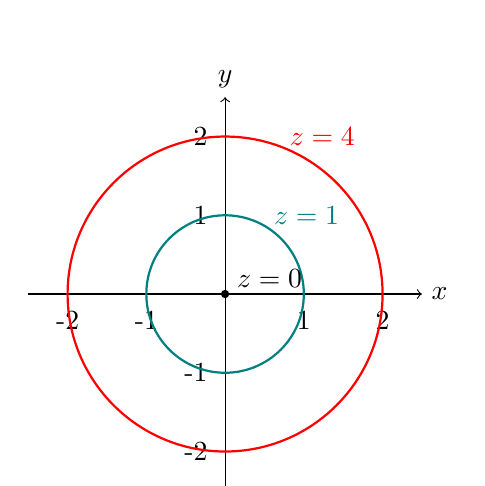
\begin{tikzpicture}[scale=1]
  % Ejes
  \draw[->] (-2.5,0) -- (2.5,0) node[right] {$x$};
  \draw[->] (0,-2.5) -- (0,2.5) node[above] {$y$};

  % Marcas y etiquetas en los ejes
  \foreach \x in {-2,-1,1,2}
    \draw (\x,0.1) -- (\x,-0.1) node[below] {\x};
  \foreach \y in {-2,-1,1,2}
    \draw (0.1,\y) -- (-0.1,\y) node[left] {\y};

  % Curvas de nivel
  % z = 0: punto en el origen
  \fill (0,0) circle (1.5pt);

  % z = 1: círculo de radio 1
  \draw[teal, thick] (0,0) circle (1);

  % z = 4: círculo de radio 2
  \draw[red, thick] (0,0) circle (2);

  % Etiquetas de curvas (fuera del dibujo)
  \node[teal,right] at (0.5,1) {$z=1$};
  \node[red,right]  at (0.7,2) {$z=4$};
  \node[right]     at (0.03,0.2) {$z=0$};
\end{tikzpicture}
\end{center}


\subsection*{2)}
No hay soluciones para $z=-1$
\begin{center}
    
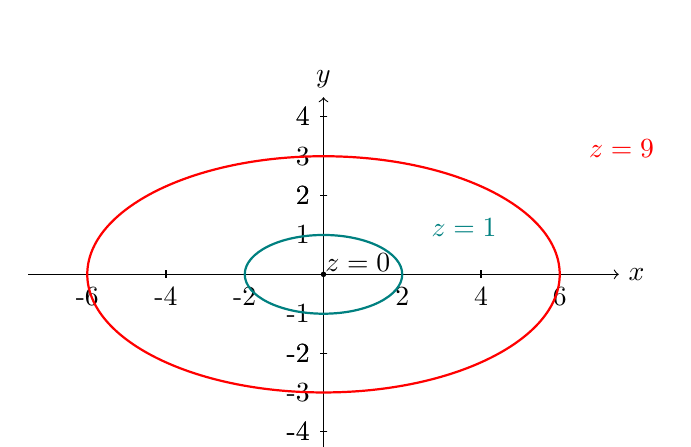
\begin{tikzpicture}[scale=0.5]
  % Ejes
  \draw[->] (-7.5,0) -- (7.5,0) node[right] {$x$};
  \draw[->] (0,-4.5) -- (0,4.5) node[above] {$y$};
  \foreach \y in {-4,-3,-2,-1,1,2,3,4}
    \draw (0.1,\y) -- (-0.1,\y) node[left] {\y};

  % Marcas y etiquetas en los ejes
  \foreach \x in {-6,-4,-2,2,4,6}
    \draw (\x,0.1) -- (\x,-0.1) node[below] {\x};
  \foreach \y in {-4,-2,2,4}
    \draw (0.1,\y) -- (-0.1,\y) node[left] {\y};

  % Curvas de nivel
  % z = 0: punto en el origen
  \fill (0,0) circle (2pt);

  % z = 1: elipse x^2/4 + y^2 = 1  => radios 2 y 1
  \draw[teal, thick] (0,0) ellipse (2cm and 1cm);

  % z = 9: elipse x^2/4 + y^2 = 9 => radios 6 y 3
  \draw[red, thick] (0,0) ellipse (6cm and 3cm);

  % Etiquetas de curvas (fuera del dibujo)
  \node[teal,right] at (2.5,1.2) {$z=1$};
  \node[red,right]  at (6.5,3.2) {$z=9$};
  \node[right]     at (-0.2,0.3) {$z=0$};
\end{tikzpicture}

\end{center}

\subsection*{3)}
\begin{center}
    
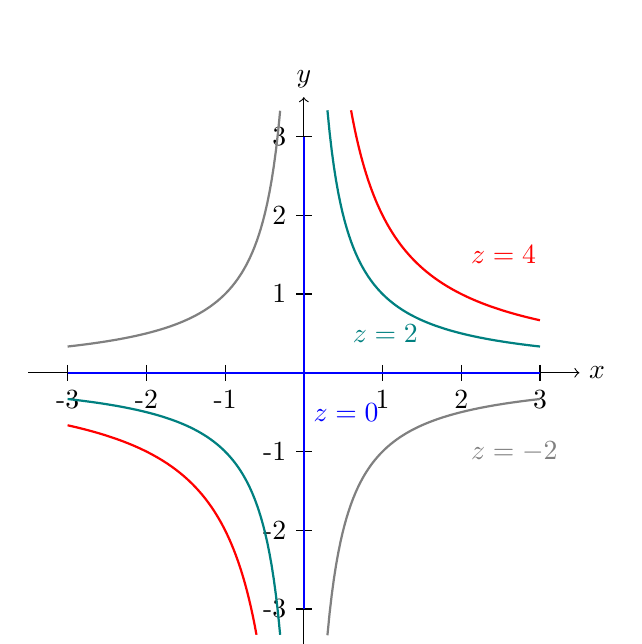
\begin{tikzpicture}[scale=1]
  % Ejes
  \draw[->] (-3.5,0) -- (3.5,0) node[right] {$x$};
  \draw[->] (0,-3.5) -- (0,3.5) node[above] {$y$};

  % Marcas y etiquetas en los ejes
  \foreach \x in {-3,-2,-1,1,2,3}
    \draw (\x,0.1) -- (\x,-0.1) node[below] {\x};
  \foreach \y in {-3,-2,-1,1,2,3}
    \draw (0.1,\y) -- (-0.1,\y) node[left] {\y};

  % Curvas de nivel de z = 2xy
  % z = 0: xy = 0  →  ejes x y y, ahora en azul
  \draw[blue, thick] (-3,0) -- (3,0);
  \draw[blue, thick] (0,-3) -- (0,3);

  % z = 2: xy = 1  →  y = 1/x
  \draw[teal, thick, domain=0.3:3,   samples=100] plot (\x,{1/\x});
  \draw[teal, thick, domain=-3:-0.3, samples=100] plot (\x,{1/\x});

  % z = 4: xy = 2  →  y = 2/x
  \draw[red,   thick, domain=0.6:3,   samples=100] plot (\x,{2/\x});
  \draw[red,   thick, domain=-3:-0.6, samples=100] plot (\x,{2/\x});

  % z = -2: xy = -1  →  y = -1/x, ahora en gris
  \draw[gray, thick, domain=0.3:3,   samples=100] plot (\x,{-1/\x});
  \draw[gray, thick, domain=-3:-0.3, samples=100] plot (\x,{-1/\x});

  % Etiquetas de curvas (fuera del dibujo)
  \node[blue,  right] at (0,-0.5)   {$z=0$};
  \node[teal,  right] at (0.5,0.5)  {$z=2$};
  \node[red,   right] at (2,1.5)   {$z=4$};
  \node[gray,  right] at (2,-1)    {$z=-2$};
\end{tikzpicture}
\end{center}


\subsection*{4)}
\begin{center}
    
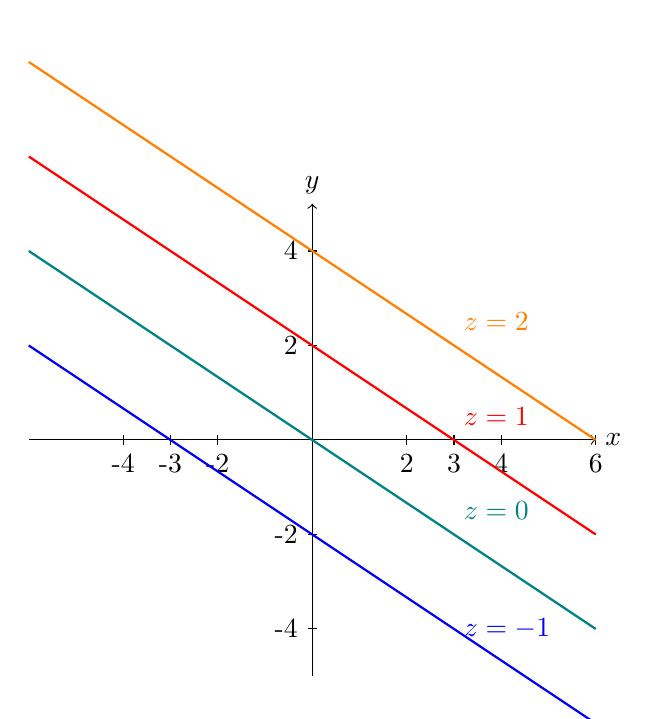
\begin{tikzpicture}[scale=0.6]
  % Ejes
  \draw[->] (-6,0) -- (6,0) node[right] {$x$};
  \draw[->] (0,-5) -- (0,5) node[above] {$y$};

  % Marcas y etiquetas en los ejes
  \foreach \x in {-4,-3,-2,2,3,4,6}
    \draw (\x,0.1) -- (\x,-0.1) node[below] {\x};
  \foreach \y in {-4,-2,2,4}
    \draw (0.1,\y) -- (-0.1,\y) node[left] {\y};

  % Curvas de nivel: 2x+3y-6z=0  ⇒ 2x+3y = 6z
  % z = -1: 2x+3y = -6  ⇒  y = -2/3 x - 2
  \draw[blue, thick, domain=-6:6] plot (\x,{-(2/3)*\x - 2});
  % z = 0: 2x+3y = 0    ⇒  y = -2/3 x
  \draw[teal, thick, domain=-6:6] plot (\x,{-(2/3)*\x});
  % z = 1: 2x+3y = 6    ⇒  y = -2/3 x + 2
  \draw[red, thick, domain=-6:6] plot (\x,{-(2/3)*\x + 2});
  % z = 2: 2x+3y = 12   ⇒  y = -2/3 x + 4
  \draw[orange, thick, domain=-6:6] plot (\x,{-(2/3)*\x + 4});

  % Etiquetas de curvas (fuera del dibujo)
  \node[blue,  right] at (3,-4)  {$z=-1$};
  \node[teal,  right] at (3,-1.5)   {$z=0$};
  \node[red,   right] at (3,0.5)   {$z=1$};
  \node[orange,right] at (3,2.5)   {$z=2$};
\end{tikzpicture}
\end{center}

\subsection*{5)}

\begin{center}
   
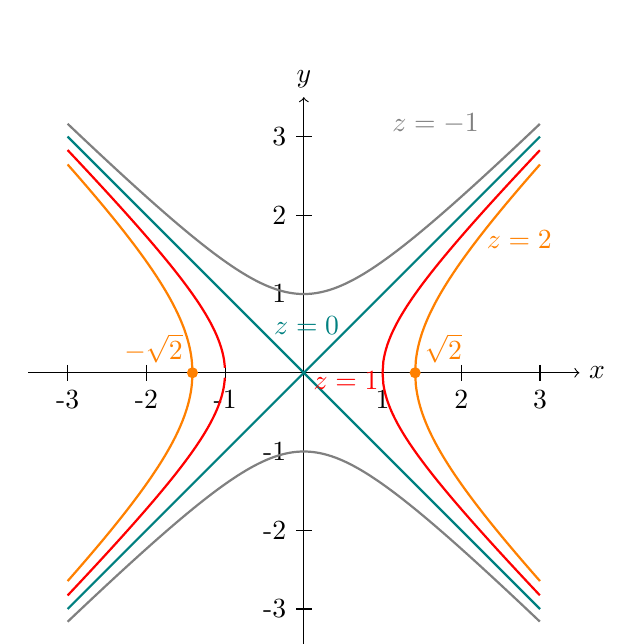
\begin{tikzpicture}[scale=1]
  % Ejes
  \draw[->] (-3.5,0) -- (3.5,0) node[right] {$x$};
  \draw[->] (0,-3.5) -- (0,3.5) node[above] {$y$};

  % Marcas y etiquetas en los ejes
  \foreach \x in {-3,-2,-1,1,2,3}
    \draw (\x,0.1) -- (\x,-0.1) node[below] {\x};
  \foreach \y in {-3,-2,-1,1,2,3}
    \draw (0.1,\y) -- (-0.1,\y) node[left] {\y};

  % Curvas de nivel de z = x^2 - y^2
  % z = -1: y = ±sqrt(x^2+1)
  \draw[gray, thick, domain=-3:3, samples=200] plot (\x,{sqrt(\x*\x+1)});
  \draw[gray, thick, domain=-3:3, samples=200] plot (\x,{-sqrt(\x*\x+1)});

  % z = 0: y = ± x
  \draw[teal, thick] (-3,-3) -- (3,3);
  \draw[teal, thick] (-3,3) -- (3,-3);

  % z = 1: y = ±sqrt(x^2-1), domain |x|>=1
  \draw[red, thick, domain=1:3, samples=200] plot (\x,{sqrt(\x*\x-1)});
  \draw[red, thick, domain=-3:-1, samples=200] plot (\x,{sqrt(\x*\x-1)});
  \draw[red, thick, domain=1:3, samples=200] plot (\x,{-sqrt(\x*\x-1)});
  \draw[red, thick, domain=-3:-1, samples=200] plot (\x,{-sqrt(\x*\x-1)});

  % z = 2: y = ±sqrt(x^2-2), domain |x|>=sqrt(2)
  \draw[orange, thick, domain={sqrt(2)}:3, samples=200] plot (\x,{sqrt(\x*\x-2)});
  \draw[orange, thick, domain=-3:-{sqrt(2)}, samples=200] plot (\x,{sqrt(\x*\x-2)});
  \draw[orange, thick, domain={sqrt(2)}:3, samples=200] plot (\x,{-sqrt(\x*\x-2)});
  \draw[orange, thick, domain=-3:-{sqrt(2)}, samples=200] plot (\x,{-sqrt(\x*\x-2)});

  % Etiquetas de curvas
  \node[gray,  right] at (1,{sqrt(3*3+1)}) {$z=-1$};
  \node[teal,  right] at (-0.5,0.6)                    {$z=0$};
  \node[red,   right] at (0,-0.1)   {$z=1$};
  \node[orange,right] at (2.2,{sqrt(2.2*2.2-2)})   {$z=2$};
    \fill[orange] ({sqrt(2)},0) circle (2pt) node[above right] {$\sqrt{2}$};
  \fill[orange] ({-sqrt(2)},0) circle (2pt) node[above left] {$-\sqrt{2}$};

\end{tikzpicture}
\end{center}



\newpage
\subsection{Ejercicio 4}

La producción de un bien está dada por
\[
z \;=\; \frac{x^2}{4} \;+\; \frac{y^2}{2}
\]
donde \(x\) e \(y\) son las cantidades de los factores de producción.

\medskip

Se pide:
\begin{enumerate}
  \item Representar las curvas de nivel (isocuantas) para
  \[
    z = 1,\quad z = 2
  \]
  \item Dar el significado de las curvas de nivel e indicar si son convexas hacia el origen, si crecen hacia arriba y a la derecha y si tienen pendiente negativa.
\end{enumerate}



\newpage
\section*{Solución}
\subsection*{1}

\begin{center}
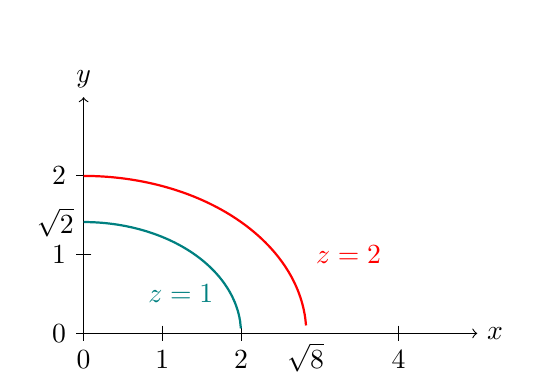
\begin{tikzpicture}[scale=1]
  % Ejes
  \draw[->] (0,0) -- (5,0) node[right] {$x$};
  \draw[->] (0,0) -- (0,3) node[above] {$y$};

  % Marcas en los ejes
  \foreach \x in {0,1,2,4}
    \draw (\x,0.1) -- (\x,-0.1) node[below] {\x};
  \foreach \y in {0,1,2}
    \draw (0.1,\y) -- (-0.1,\y) node[left] {\y};

  % Isocuanta z = 1: x^2/4 + y^2/2 = 1  (primer cuadrante)
  \draw[teal, thick, domain=0:2, samples=200]
    plot (\x,{ sqrt(2 - \x*\x/2) });

  % Isocuanta z = 2: x^2/4 + y^2/2 = 2  (primer cuadrante)
  \draw[red, thick, domain=0:{2*sqrt(2)}, samples=500]
    plot (\x,{ sqrt(4 - \x*\x/2) });

  % Etiquetas
  \node[teal, right] at (0.7,0.5)   {$z=1$};
  
  \node[red,   right] at ({2*sqrt(2)},1) {$z=2$};
    \node[black, left] at (0,1.41)   {$\sqrt{2}$};
    \node[black, below] at (2.82,0)   {$\sqrt{8}$};

\end{tikzpicture}
\end{center}

\subsection*{2}
\textbf{\color{teal}Las curvas cumplen crecen hacia arriba y a la derecha, son tienen pendiente negativa pero no son convexas al origen.
}

\newpage

\subsection{Ejercicio 5}
Dada la función de producción \( z = 6xy \), donde \( x \) es el número de máquinas usadas y \( y \) es el número de horas hombre, se pide:

\begin{enumerate}
  \item Determinar las curvas de producción constante para \( z = 6 \), \( z = 18 \). Representar gráficamente.
  
  \item Si se desea obtener un volumen de producción de 300 unidades y se dispone de dos máquinas, ¿cuántas horas hombre se necesitan?

  \item Si se deben producir 6000 unidades con 200 horas hombre, ¿cuántas máquinas se deben utilizar?
\end{enumerate}

\newpage
\section*{Solución}

\subsection*{1. Curvas de producción constante}

La isocuanta (curva de producción constante) para un nivel \(z_0\) viene dada por
\[
z_0 = 6\,x\,y
\quad\Longrightarrow\quad
y = \frac{z_0}{6x}
\]
Por lo tanto:
\begin{itemize}
  \item Para \(z = 6\):
  \[
  \color{teal} y = \frac{6}{6x} = \frac{1}{x}
  \]
  \item Para \(z = 18\):
  \[
  \color{teal} y = \frac{18}{6x} = \frac{3}{x}
  \]
\end{itemize}

\bigskip

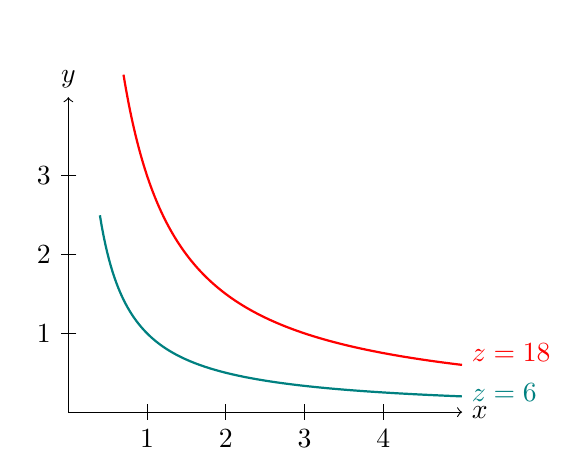
\begin{tikzpicture}[scale=1]
  % Ejes
  \draw[->] (0,0) -- (5,0) node[right] {$x$};
  \draw[->] (0,0) -- (0,4) node[above] {$y$};

  % Marcas en los ejes
  \foreach \x in {1,2,3,4}
    \draw (\x,0.1) -- (\x,-0.1) node[below] {\x};
  \foreach \y in {1,2,3}
    \draw (0.1,\y) -- (-0.1,\y) node[left] {\y};

  % Iso­cuanta z=6: y=1/x
  \draw[teal, samples=200, domain=0.4:5, thick]
    plot (\x,{1/\x});
  % Iso­cuanta z=18: y=3/x
  \draw[red, samples=200, domain=0.7:5, thick]
    plot (\x,{3/\x});

  % Etiquetas de curvas
  \node[teal, right] at (5,0.25)   {$z = 6$};
  \node[red,   right] at (5,0.75)  {$z = 18$};
\end{tikzpicture}

\subsection*{2. Horas hombre necesarias para \(z = 300\) con \(x = 2\)}

Dada la función \(z = 6xy\), fijamos \(x = 2\) y \(z = 300\)
\[
\color{teal}
6 \cdot 2 \cdot y = 300
\quad\Longrightarrow\quad
y = \frac{300}{12} = 25
\]
\textcolor{teal}{Por tanto, se necesitan \(25\) horas hombre}

\bigskip

\subsection*{3. Máquinas necesarias para \(z = 6000\) con \(y = 200\)}

Fijando \(y = 200\) y \(z = 6000\):
\[
\color{teal}
6x \cdot 200 = 6000
\quad\Longrightarrow\quad
x = \frac{6000}{1200} = 5
\]
\textcolor{teal}{Por tanto, se deben emplear \(5\) máquinas}

\newpage

\subsection{Ejercicio 6}

Si la función de utilidad es \( U = 3x_1 x_2 \) y, además, \( p_1 = 5 \), \( p_2 = 6 \) se pide:

\begin{enumerate}
    \item Hallar la ecuación de balance.
    \item Hallar la máxima utilidad si \( R = 120 \). Graficar.
\end{enumerate}

\newpage
\section*{Solución}

\subsection*{1. Ecuación de balance}

La restricción presupuestaria es
\[
\color{teal}
5x_1 + 6x_2 = R = 120
\]

\subsection*{2. Maximización de la utilidad}

\paragraph{a) Curva de indiferencia}

Para \(U = \bar U\) constante:
\[
3x_1x_2 = \bar U
\quad\Longrightarrow\quad
x_1 = \frac{\bar U}{3x_2},
\quad
\frac{dx_1}{dx_2}\Big|_{U} = -\frac{\bar U}{3x_2^2}
\]

\paragraph{b) Recta presupuestaria}

Despejando \(x_1\):
\[
x_1 = \frac{120 - 6x_2}{5},
\quad
\frac{dx_1}{dx_2}\Big|_{B} = -\frac{6}{5}
\]

\paragraph{c) Igualación de pendientes}
\[
-\frac{\bar U}{3x_2^2} = -\frac{6}{5}
\quad\Longrightarrow\quad
\bar U = \frac{18}{5} x_2^2
\]

\paragraph{d) Derivadas \(\frac{dx_2}{dx_1}\)}

De \(3x_1x_2 = \bar U\):
\[
x_2 = \frac{\bar U}{3x_1},
\quad
\frac{dx_2}{dx_1}\Big|_{U} = -\frac{\bar U}{3x_1^2}
\]

De \(5x_1 + 6x_2 = 120\):
\[
x_2 = \frac{120 - 5x_1}{6},
\quad
\frac{dx_2}{dx_1}\Big|_{B} = -\frac{5}{6}
\]

\paragraph{e) Segunda igualación de pendientes}
\[
-\frac{\bar U}{3x_1^2} = -\frac{5}{6}
\quad\Longrightarrow\quad
\bar U = \frac{5}{2} x_1^2
\]
Igualando las dos expresiones de \(\bar U\):
\[
\frac{18}{5} x_2^2 = \frac{5}{2} x_1^2
\quad\Longrightarrow\quad
x_2^2 = \frac{25}{18} x_1^2
\quad\Longrightarrow\quad
x_2 = \frac{5}{\sqrt{18}} x_1
= \frac{5}{3\sqrt{2}} x_1
\]
pero para simplificar usamos la primera relación obtenida:
\[
\color{teal}
3x_1 = \frac{18}{5} x_2
\;\Longrightarrow\;
x_2 = \frac{5}{6} x_1
\]

\paragraph{f) Cálculo de la solución óptima}

Sustituimos \(x_2 = \tfrac{5}{6}x_1\) en la restricción:
\[
\color{teal}
5x_1 + 6\left(\tfrac{5}{6}x_1\right) = 10x_1 = 120
\;\Longrightarrow\;
x_1^* = 12,
\quad
x_2^* = \tfrac{5}{6} \cdot 12 = 10
\]
La máxima utilidad es
\[
\color{teal}
U_{\max} = 3 \cdot 12 \cdot 10 = 360
\]

\subsection*{Gráfico}

\begin{center}
\begin{tikzpicture}[scale=0.2]
  % Ejes
  \draw[->] (0,0) -- (30,0) node[right] {$x_1$};
  \draw[->] (0,0) -- (0,30) node[above] {$x_2$};
  % Marcas
  \foreach \x in {0,5,10,15,20,25}
    \draw (\x,0.5) -- (\x,-0.5) node[below] {\x};
  \foreach \y in {0,5,10,15,20}
    \draw (0.5,\y) -- (-0.5,\y) node[left] {\y};
  % Recta presupuestaria: x2 = (120 - 5*x1)/6
  \draw[blue, thick] plot[domain=0:24] (\x,{(120-5*\x)/6});
  % Indiferencia U=360: x2 = 360/(3*x1) = 120/x1
  \draw[teal, thick, domain=5:30, samples=200] plot (\x,{120/\x});
  \node[teal, right] at (30,5) {$U = 360$};
  % Óptimo (12,10)
  \fill (12,10) circle (3pt) node[above right] {$(12,10)$};
\end{tikzpicture}
\end{center}

\newpage

\subsection{Ejercicio 7}

Un productor de quesos utiliza como insumo \( x \) cantidad de leche en la producción de dos tipos de quesos \( A \) y \( B \). 
Si la función de producción conjunta está dada por
\[
x = 4q_1^2 + 2q_2^2
\]
donde \( q_1 \) y \( q_2 \) son las cantidades de queso del tipo \( A \) y \( B \) respectivamente, producidas en forma conjunta con \( x \) cantidad de leche y, además, el precio de cada tipo de queso es 3 y 4 respectivamente, se pide:

\begin{enumerate}
    \item Hallar la función de ingreso total.
    \item Graficar las líneas de isongreso.
    \item Dar el valor máximo de ingreso obtenido con 164 toneladas de leche.
\end{enumerate}
\newpage
\section*{Solución}


%%%%%%%%%%%


\subsection*{(1) Función de ingreso total}

Sea \(p_1 = 3\) el precio por unidad del queso tipo \(A\) y \(p_2 = 4\) el precio por unidad del queso tipo \(B\). 
Las cantidades producidas de cada tipo de queso se denotan por \(q_1\) y \(q_2\). 

La función de ingreso total \(R\) se obtiene multiplicando los precios por las cantidades producidas:
\[\color{teal}
R = p_1 \, q_1 + p_2 \, q_2 = 3\,q_1 + 4\,q_2
\]

\subsection*{(2) Líneas de isongreso}

Las líneas de isongreso se obtienen al fijar un nivel de ingreso \(R = \bar{R}\) y representar la relación entre \(q_1\) y \(q_2\). Dado que
\[
R = 3\,q_1 + 4\,q_2
\]
una línea de isongreso para un ingreso constante \(\bar{R}\) se describe por
\[
3\,q_1 + 4\,q_2 = \bar{R}
\]
Despejando \(q_2\) en función de \(q_1\):
\[\color{teal}
q_2 = \frac{\bar{R} - 3\,q_1}{4}
\]
Esta es la ecuación de una recta con intercepto \(\bar{R}/4\) en el eje \(q_2\) y pendiente \(-3/4\).
\begin{center}
% Note: TikZ code remains unchanged as it's graphical generation
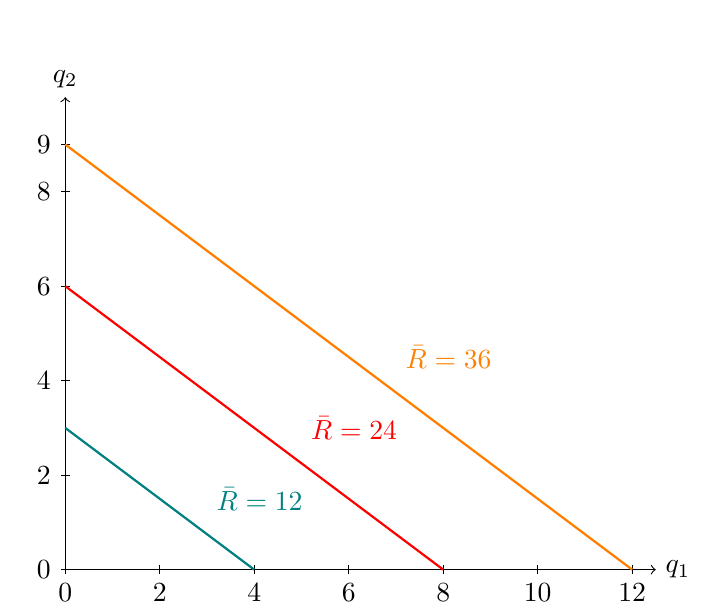
\begin{tikzpicture}[scale=0.6]
 % Ejes
 \draw[->] (0,0) -- (12.5,0) node[right] {$q_1$};
 \draw[->] (0,0) -- (0,10)   node[above] {$q_2$};

 % Marcas en ejes
 \foreach \x in {0,2,4,6,8,10,12}
  \draw (\x,0.1) -- (\x,-0.1) node[below] {\x};
 \foreach \y in {0,2,4,6,8,9}
  \draw (0.1,\y) -- (-0.1,\y) node[left] {\y};

 % Línea R=12
 \draw[teal, thick, domain=0:4] plot (\x,{(12 - 3*\x)/4});
 % Línea R=24
 \draw[red, thick,  domain=0:8] plot (\x,{(24 - 3*\x)/4});
 % Línea R=36
 \draw[orange, thick, domain=0:12] plot (\x,{(36 - 3*\x)/4});

 % Etiquetas
 \node[teal,  right]  at (3,1.5)  {$\bar R=12$};
 \node[red,   right]  at (5,3)   {$\bar R=24$};
 \node[orange,right]  at (7,4.5) {$\bar R=36$};
\end{tikzpicture}
\end{center}

\subsection*{(3) Valor máximo de ingreso con \(x = 164\) toneladas de leche}

% Note: The description "toneladas de leche" implies x is the resource constraint.
% The constraint appears to be 4q_1^2 + 2q_2^2 = 164 based on the derivatives section.

\bigskip
\paragraph{Derivadas de la restricción}

\begin{enumerate}
    \item \textbf{Despejando \(q_1\) en función de \(q_2\):}  
    De la restricción tenemos
    \[
    4q_1^2 = 164 - 2q_2^2 
    \quad \Longrightarrow \quad 
    q_1 = \frac{1}{2}\sqrt{164 - 2q_2^2}
    \]
    Derivando con respecto a \(q_2\):
    \[
    \frac{dq_1}{dq_2} = \frac{1}{2}\cdot\frac{1}{2\sqrt{164-2q_2^2}}\cdot(-4q_2)
    = -\frac{q_2}{\sqrt{164-2q_2^2}}
    \]
    
    \item \textbf{Despejando \(q_2\) en función de \(q_1\):}  
    De la restricción
    \[
    2q_2^2 = 164 - 4q_1^2 
    \quad \Longrightarrow \quad 
    q_2 = \sqrt{\frac{164-4q_1^2}{2}}
    = \sqrt{82 - 2q_1^2}
    \]
    Derivando con respecto a \(q_1\):
    \[
    \frac{dq_2}{dq_1} 
    = \frac{1}{2\sqrt{82-2q_1^2}} \cdot (-4q_1)
    = -\frac{2q_1}{\sqrt{82-2q_1^2}}
    \]
\end{enumerate}

\bigskip
\paragraph{Derivadas de la función de ingreso}

La función de ingreso es:
\[
R = 3q_1 + 4q_2
\]
Consideramos las dos formas de despejar las variables a partir de una línea de isongreso (nivel constante de ingreso):



%%%%%%%%%%


\begin{enumerate}
    \item \textbf{Despejando \(q_1\) en función de \(q_2\):}  
    Sea \(R = \bar{R}\) constante. Entonces,
    \[
    3q_1 = \bar{R} - 4q_2 
    \quad \Longrightarrow \quad 
    q_1 = \frac{\bar{R} - 4q_2}{3}
    \]
    Derivando con respecto a \(q_2\):
    \[
    \frac{dq_1}{dq_2} = -\frac{4}{3}
    \]
    
    \item \textbf{Despejando \(q_2\) en función de \(q_1\):}  
    De \(3q_1 + 4q_2 = \bar{R}\), se tiene:
    \[
    q_2 = \frac{\bar{R} - 3q_1}{4}
    \]
    Derivando con respecto a \(q_1\):
    \[
    \frac{dq_2}{dq_1} = -\frac{3}{4}
    \]
\end{enumerate}

\bigskip
\paragraph{Igualación de pendientes}

La condición de optimalidad requiere que la pendiente de la restricción (derivada obtenida al despejar) sea igual a la pendiente de la línea de isongreso.

Podemos igualar, por ejemplo, la derivada obtenida al despejar \(q_2\) en función de \(q_1\):

De la restricción tenemos:
\[
\frac{dq_2}{dq_1} = -\frac{2q_1}{\sqrt{82-2q_1^2}}
\]
y de la línea de isongreso:
\[
\frac{dq_2}{dq_1} = -\frac{3}{4}
\]

Igualamos (sin los signos negativos):
\[
\frac{2q_1}{\sqrt{82-2q_1^2}} = \frac{3}{4}
\]

Multiplicamos ambos lados por \(\sqrt{82-2q_1^2}\) y por 4:
\[
8q_1 = 3\sqrt{82-2q_1^2}
\]

Elevamos al cuadrado ambos lados:
\[
64q_1^2 = 9(82-2q_1^2)
\]

Expandiendo y reuniendo términos:
\[
64q_1^2 = 738 - 18q_1^2 
\quad \Longrightarrow \quad 
64q_1^2 + 18q_1^2 = 738 
\quad \Longrightarrow \quad 
82q_1^2 = 738
\]

Dividiendo entre 82:
\[
q_1^2 = \frac{738}{82} = 9 
\quad \Longrightarrow \quad 
\color{teal} q_1 = 3 \quad (\text{se toma la solución positiva})
\]

Con \(q_1 = 3\), sustituimos en la restricción para obtener \(q_2\):
\[
4(3)^2 + 2q_2^2 = 164 
\quad \Longrightarrow \quad 
36 + 2q_2^2 = 164
\]
Restando 36:
\[ 
2q_2^2 = 128 
\quad \Longrightarrow \quad 
q_2^2 = 64 
\quad \Longrightarrow \quad 
\color{teal} q_2 = 8 \quad (\text{se toma la solución positiva})
\]

Sustituyendo en la función de ingreso:
\[
R_{\max} = 3q_1 + 4q_2 = 3\cdot 3 + 4\cdot 8 = 9 + 32 = \color{teal} 41
\]
%%%%%%%%%%%%%%%%%%%

\subsection*{Otra forma de encontrar maximizar}

Recordemos que el problema es maximizar el ingreso
\[
R = 3\,q_1 + 4\,q_2
\]
sujeto a la restricción 
\[
4\,q_1^2 + 2\,q_2^2 = 164
\]

En lugar de utilizar el método de Lagrange, vamos a \textbf{despejar una variable} de la restricción y luego \textbf{substituirla} en la función objetivo, de modo que el problema quede en una sola variable.

\subsection*{Despeje de \(q_2\) a partir de la restricción}

La restricción es:
\[
4\,q_1^2 + 2\,q_2^2 = 164
\]
Despejamos \(q_2^2\):
\[
2\,q_2^2 = 164 - 4\,q_1^2
\;\;\Longrightarrow\;\;
q_2^2 = \frac{164 - 4\,q_1^2}{2} = 82 - 2\,q_1^2
\]
Suponiendo \(q_2 \ge 0\) (pues las cantidades físicas de queso no pueden ser negativas), tenemos
\[
q_2 = \sqrt{82 - 2\,q_1^2}
\]

\subsection*{Función objetivo en términos de \(q_1\)}

Sustituyendo \(q_2\) en la función de ingreso \(R\), obtenemos
\[
R(q_1) 
= 3\,q_1 + 4\,q_2 
= 3\,q_1 + 4 \sqrt{\,82 - 2\,q_1^2\,}
\]


\subsection*{Maximización en una variable}

Para hallar el valor de \(q_1\) que maximiza \(R(q_1)\), derivamos \(R\) con respecto a \(q_1\) y buscamos los puntos críticos en el intervalo anterior.

\[
R(q_1) = 3\,q_1 + 4\,\sqrt{\,82 - 2\,q_1^2\,}
\]
Calculemos la derivada \(R'(q_1)\). Para la segunda parte, notemos que si definimos 
\(\displaystyle f(q_1) = 82 - 2\,q_1^2\)
entonces 
\(\displaystyle \sqrt{f(q_1)} = \sqrt{82 - 2\,q_1^2}\)

\[
R'(q_1) 
= \frac{d}{dq_1}\Bigl[\,3\,q_1\Bigr] 
  \;+\; 4 \,\frac{d}{dq_1}\Bigl[\sqrt{f(q_1)}\Bigr]
\]
La primera parte es simplemente \(3\). Para la segunda parte:
\[
\frac{d}{dq_1}\Bigl[\sqrt{f(q_1)}\Bigr]
= \frac{1}{2\,\sqrt{f(q_1)}} \,\frac{d}{dq_1}\bigl[f(q_1)\bigr]
= \frac{1}{2\,\sqrt{82 - 2\,q_1^2}} \,(-4\,q_1)
\]
pues \(\frac{d}{dq_1}[82 - 2\,q_1^2] = -4\,q_1\)

Por tanto,
\[
R'(q_1) 
= 3 
  \;+\; 4 \cdot \left(\frac{-4\,q_1}{2\,\sqrt{82 - 2\,q_1^2}}\right)
= 3 \;-\; \frac{16\,q_1}{2\,\sqrt{82 - 2\,q_1^2}}
= 3 \;-\; \frac{8\,q_1}{\sqrt{82 - 2\,q_1^2}}
\]

\subsection*{5. Punto crítico}

Para un máximo local, buscamos \(R'(q_1) = 0\):
\[
3 \;-\; \frac{8\,q_1}{\sqrt{82 - 2\,q_1^2}} = 0
\;\;\Longrightarrow\;\;
3 = \frac{8\,q_1}{\sqrt{82 - 2\,q_1^2}}
\]
Despejamos \(\sqrt{82 - 2\,q_1^2}\):
\[
\sqrt{82 - 2\,q_1^2} 
= \frac{8\,q_1}{3}
\]
Elevando al cuadrado ambos lados:
\[
82 - 2\,q_1^2 
= \left(\frac{8\,q_1}{3}\right)^2
= \frac{64\,q_1^2}{9}
\]
Pasamos todo a un lado:
\[
82 
= 2\,q_1^2 + \frac{64\,q_1^2}{9}
= 2\,q_1^2 + \frac{64}{9}\,q_1^2
= \left(2 + \frac{64}{9}\right) q_1^2
= \frac{18}{9}\,q_1^2 + \frac{64}{9}\,q_1^2
= \frac{82}{9}\,q_1^2
\]
De modo que
\[
82 
= \frac{82}{9}\,q_1^2
\;\;\Longrightarrow\;\;
q_1^2 = 9
\;\;\Longrightarrow\;\;
\color{teal} q_1 = 3
\quad (\text{tomamos la raíz positiva, }q_1 \ge 0)
\]

\subsection*{Valor de \(q_2\)}

Con \(q_1 = 3\), hallamos \(q_2\) de la restricción:
\[
4\,q_1^2 = 4 \cdot 9 = 36
\]
\[
2\,q_2^2 = 164 - 36 = 128
\;\;\Longrightarrow\;\;
q_2^2 = 64
\;\;\Longrightarrow\;\;
\color{teal} q_2 = 8
\quad (\text{tomando la raíz positiva})
\]

\subsection*{Ingreso máximo}

Evaluamos la función de ingreso en \((q_1, q_2) = (3, 8)\):
\[
R_{\max} = 3\,\cdot\,3 + 4\,\cdot\,8 = 9 + 32 = \color{teal} 41
\]



\newpage

\subsection{Ejercicio 8}


 En un proceso de producción simple, un empresario utiliza dos insumos \(x_1\) y \(x_2\) para producir un solo producto, 
siendo la función de producción que establece la cantidad de producto 
\[
q = x_1 \, x_2
\]
Si el costo unitario de cada insumo es 3 y 6, respectivamente, y existe un costo fijo de 180 unidades monetarias, se pide:

\begin{enumerate}
    \item Hallar la función de costo total.
    \item Hallar el valor del mínimo costo total para un producto de \(q = 2\).
\end{enumerate}



%%%%%%%%%%%%%%%%%%%

\newpage
\section*{Solución}

\subsection*{Función de costo total}

Dado que el costo unitario del insumo \(x_1\) es 3 y el del insumo \(x_2\) es 6, y además existe un costo fijo de 180, la \textbf{función de costo total} se escribe como:
\[
C = 3\,x_1 + 6\,x_2 + 180
\]

\bigskip

\subsection*{Costo mínimo para producir \(q=2\)}

El problema consiste en \emph{minimizar}
\[
C = 3\,x_1 + 6\,x_2 + 180
\]
sujeto a la \emph{restricción}
\[
x_1 \, x_2 = 2
\]
Para encontrar el \emph{costo mínimo}, podemos:

\begin{enumerate}
    \item Despejar una variable de la restricción
    \item Sustituir en la función de costo, reduciendo el problema a una sola variable
    \item Hallar el valor de dicha variable que minimiza el costo
    \item Calcular el costo correspondiente
\end{enumerate}

\paragraph{1) Despeje de la restricción}

De \(x_1 \, x_2 = 2\), podemos, por ejemplo, \textbf{despejar} \(x_2\):
\[
x_2 = \frac{2}{x_1}
\]

\paragraph{2) Sustitución en la función de costo}

Sustituyendo \(x_2 = \frac{2}{x_1}\) en \(C\), obtenemos:
\[
C(x_1) = 3\,x_1 + 6\left(\frac{2}{x_1}\right) + 180
       = 3\,x_1 + \frac{12}{x_1} + 180
\]

\paragraph{3) Minimización de \(C(x_1)\)}

Para hallar el mínimo, derivamos con respecto a \(x_1\) y \emph{igualamos a cero}:
\[
\frac{dC}{dx_1}
= 3 - \frac{12}{x_1^2} = 0
\]
Despejamos:
\[
3 = \frac{12}{x_1^2}
\quad \Longrightarrow \quad
x_1^2 = \frac{12}{3} = 4
\quad \Longrightarrow \quad
\color{teal}{x_1 = 2}
\quad (\text{tomamos la raíz positiva, pues } x_1 > 0)
\]

\paragraph{4) Valor de \(x_2\)}

Con \(x_1 = 2\), la restricción \(x_1 \, x_2 = 2\) da:
\[
2 \cdot x_2 = 2
\quad \Longrightarrow \quad
\color{teal}{x_2 = 1}
\]

\paragraph{5) Costo mínimo}

Sustituyendo \((x_1, x_2) = (2,1)\) en la función de costo:
\[
C_{\min}
= 3\cdot 2 + 6\cdot 1 + 180
= 6 + 6 + 180
= \color{teal}{192}
\]


%%%%%%%%%%%%%%%%

\bigskip

\subsection*{Costo mínimo para producir \(q = 2\) mediante igualación de pendientes}

Dado el problema:
\[
\min \; C = 3\,x_1 + 6\,x_2 + 180
\quad \text{sujeto a} \quad
x_1\,x_2 = 2
\]
podemos resolverlo \emph{igualando las pendientes} de la \textbf{iso-costo} y la \textbf{iso-cuanta} (o \textbf{curva de nivel} de la función de producción).

\bigskip

\subsection*{1) Restricción (iso-cuanta)}

\begin{enumerate}
    \item \textbf{Despejando \(x_1\) en función de \(x_2\):}
    \[
    x_1 = \frac{2}{x_2}
    \]
    Derivando con respecto a \(x_2\):
    \[
    \frac{dx_1}{dx_2}
    = -\,\frac{2}{x_2^2}
    \]

    \item \textbf{Despejando \(x_2\) en función de \(x_1\):}
    \[
    x_2 = \frac{2}{x_1}
    \]
    Derivando con respecto a \(x_1\):
    \[
    \frac{dx_2}{dx_1}
    = -\,\frac{2}{x_1^2}
    \]
\end{enumerate}

\bigskip

\subsection*{2) Función de costo (iso-costo)}

Las \emph{líneas de iso-costo} (para un costo total \(C\) constante) se describen por:
\[
3\,x_1 + 6\,x_2 = \text{Constante}
\]
Para llamarla \(\bar{C}\), tenemos
\[
3\,x_1 + 6\,x_2 = \bar{C}
\]

\begin{enumerate}
    \item \textbf{Despejando \(x_1\) en función de \(x_2\):}
    \[
    x_1 = \frac{\bar{C} - 6\,x_2}{3}
    \]
    Derivando con respecto a \(x_2\):
    \[
    \frac{dx_1}{dx_2}
    = -\,\frac{6}{3}
    = -\,2
    \]

    \item \textbf{Despejando \(x_2\) en función de \(x_1\):}
    \[
    x_2 = \frac{\bar{C} - 3\,x_1}{6}
    \]
    Derivando con respecto a \(x_1\):
    \[
    \frac{dx_2}{dx_1}
    = -\,\frac{3}{6}
    = -\,\frac{1}{2}
    \]
\end{enumerate}

\bigskip

\subsection*{3) Igualación de pendientes}

Para el \emph{óptimo}, la curva de iso-costo debe ser \emph{tangente} a la iso-cuanta. Eso implica que sus pendientes coincidan. Tenemos dos maneras de igualar pendientes (usando cualquiera de las dos formas de despeje):

\begin{itemize}
    \item \(\displaystyle \frac{dx_1}{dx_2}\) de la restricción \(=\) \(\displaystyle \frac{dx_1}{dx_2}\) de la iso-costo
    \item \(\displaystyle \frac{dx_2}{dx_1}\) de la restricción \(=\) \(\displaystyle \frac{dx_2}{dx_1}\) de la iso-costo
\end{itemize}

\paragraph{Usando \(\tfrac{dx_1}{dx_2}\)}

\[
-\frac{2}{x_2^2} \;=\; -2
\quad \Longrightarrow \quad
\frac{2}{x_2^2} = 2
\quad \Longrightarrow \quad
x_2^2 = 1
\quad \Longrightarrow \quad
\color{teal}{x_2 = 1} \; (\text{el valor positivo})
\]
De la restricción \(x_1\,x_2 = 2\):
\[
x_1 \cdot 1 = 2
\quad \Longrightarrow \quad
\color{teal}{x_1 = 2}
\]

\paragraph{Usando \(\tfrac{dx_2}{dx_1}\)}

\[
-\frac{2}{x_1^2} \;=\; -\frac{1}{2}
\quad \Longrightarrow \quad
\frac{2}{x_1^2} = \frac{1}{2}
\quad \Longrightarrow \quad
x_1^2 = 4
\quad \Longrightarrow \quad
\color{teal}{x_1 = 2} \; (\text{positivo})
\]
Nuevamente, de \(x_1\,x_2 = 2\):
\[
2 \cdot x_2 = 2
\quad \Longrightarrow \quad
\color{teal}{x_2 = 1}
\]

{\color{teal}Ambas vías coinciden en \((x_1, x_2) = (2,\,1)\)}
%%%%%%%%%%%%%%%

\newpage
\subsection{Ejercicio 9}
Una función de producción está dada por $q=x^{1/2}y^{1/2}$ donde $x$ e $y$ son las cantidades de insumos cuya función de costo total está dada por $x+2y+100=C$. Determinar gráfica y analíticamente utilizando las curvas de nivel la máxima producción que puede obtener el productor si dispone de un costo total de 124.

\newpage
\section*{Respuesta}
Obtenemos primero la pendiente de la curva de nivel de la función a maximizar:
\begin{equation*}
\bar{q}=x^{1/2}y^{1/2}
\end{equation*}
\begin{equation*}
\dfrac{\bar{q}^2}{y}=x
\end{equation*}
\begin{equation*}
x'y= -\dfrac{\bar{q}^2}{y^2}
\end{equation*}
\begin{equation*}
\dfrac{\bar{q}^2}{x}=y
\end{equation*}
\begin{equation*}
y'x= -\dfrac{\bar{q}^2}{x^2}
\end{equation*}
La pendiente entonces es el cociente de derivadas:
\begin{equation*}
\dfrac{x'y}{y'x}=\dfrac{-\dfrac{\bar{q}^2}{y^2}}{ -\dfrac{\bar{q}^2}{x^2}}=\dfrac{x^2}{y^2}
\end{equation*}
Obtenemos la pendiente de la curva de nivel de la restricción:
\begin{equation*}
x+2y+100=C
\end{equation*}
\begin{equation*}
x=C-100-2y
\end{equation*}
\begin{equation*}
x'y=-2
\end{equation*}
\begin{equation*}
y=C/2-100/2-x/2
\end{equation*}
\begin{equation*}
y'x=-1/2
\end{equation*}
La pendiente entonces es el cociente de derivadas:
\begin{equation*}
\dfrac{x'y}{y'x}=\dfrac{-2}{-1/2}=4
\end{equation*}
Igualamos las pendientes de las curvas de nivel:
\begin{equation*}
\dfrac{x^2}{y^2}=4
\end{equation*}
Despejo una variable:
\begin{equation*}
x=2y
\end{equation*}
Inserto en la restricción:
\begin{equation*}
{\color{teal} 2y}+2y+100=124
\end{equation*}
\begin{equation*}
4y=24
\end{equation*}
\begin{equation*}
\color{teal}y=6
\end{equation*}
Inserto esto en la ecuación de $x$
\begin{equation*}\color{teal}
x=2 \cdot{\color{teal} 6}=12
\end{equation*}
Calculamos la producción:
\begin{equation*}
12^{1/2}6^{1/2}= \color{teal} 72^{1/2}
\end{equation*}

\begin{tikzpicture}[scale=0.4]
  % Ejes
  \draw[->] (0,0) -- (26,0) node[right] {$x$};
  \draw[->] (0,0) -- (0,14) node[above] {$y$};

  % Marcas en los ejes
  \foreach \x in {0,6,12,18,24}
    \draw (\x,0.2) -- (\x,-0.2) node[below] {\x};
  \foreach \y in {0,3,6,9,12}
    \draw (0.2,\y) -- (-0.2,\y) node[left] {\y};

  % Isocosto: y = (24 - x)/2
  \draw[blue, thick, domain=0:24] plot (\x,{(24-\x)/2});
  \node[blue, right] at (24,0) {};

  % Isocuanta óptima: y = 72/x
  \draw[teal, thick, domain=4:24, samples=200] plot (\x,{72/\x});
  \node[red, right] at (24,{72/24+0.5}) {isocuanta $q=\sqrt{72}$};

  % Punto óptimo (12,6)
  \fill (12,6) circle (4pt) node[above right] {$(12,6)$};

\end{tikzpicture}

\newpage

\subsection{Ejercicio 10}



Dada la función de utilidad 
\[
U(q_1, q_2) = q_1 \cdot q_2
\]
de un consumidor con la restricción presupuestaria
\[
2q_1 + 5q_2 = 100.
\]

\begin{enumerate}
    \item Hallar las cantidades \(q_1\) y \(q_2\) que maximizan la utilidad y calcular a cuánto asciende esta.
    \item Graficar la curva de indiferencia de la función de utilidad dada, la recta presupuestaria y el punto en donde se maximiza la utilidad.
\end{enumerate}
\newpage
\section*{Solución}

\subsection*{1. Fijar el nivel óptimo}
En el óptimo se asume que la utilidad es constante:
\[
q_1 \cdot q_2 = K,
\]
donde \(K\) es el nivel de utilidad alcanzado en el óptimo.

\subsection*{2. Despejar \(q_1\) en función de \(q_2\)}
\begin{itemize}
    \item \textbf{Desde la función de utilidad:}  
    \[
    q_1 = \frac{K}{q_2}
    \]
    \item \textbf{Desde la restricción presupuestaria:}  
    \[
    2q_1 + 5q_2 = 100 \quad \Longrightarrow \quad q_1 = \frac{100 - 5q_2}{2}
    \]
\end{itemize}

\subsection*{3. Derivar respecto a \(q_2\)}
Derivamos ambas expresiones respecto a \(q_2\):

\begin{itemize}
    \item \textbf{Desde la función de utilidad:}
    \[
    \frac{dq_1}{dq_2}\Big|_{\text{utilidad}} = -\frac{K}{q_2^2}
    \]
    \item \textbf{Desde la restricción:}
    \[
    \frac{dq_1}{dq_2}\Big|_{\text{restricción}} = -\frac{5}{2}
    \]
\end{itemize}

\subsection*{4. Igualar las derivadas}
En el punto óptimo ambas pendientes deben coincidir, es decir:
\[
-\frac{K}{q_2^2} = -\frac{5}{2}
\]
Cancelamos el signo negativo:
\[
\frac{K}{q_2^2} = \frac{5}{2},
\]
de donde se obtiene:
\[ \color{teal}
K = \frac{5}{2}\,q_2^2
\]


\subsection*{5. Derivar respecto a \(q_1\) y despejar \(K\) también}

Análogamente, despejamos \(q_2\) en función de \(q_1\):

\begin{itemize}
    \item \textbf{Desde la función de utilidad:}
    \[
    q_1 \cdot q_2 = K \quad \Longrightarrow \quad q_2 = \frac{K}{q_1}
    \]
    \item \textbf{Desde la restricción presupuestaria:}
    \[
    2q_1 + 5q_2 = 100 \quad \Longrightarrow \quad q_2 = \frac{100 - 2q_1}{5}
    \]
\end{itemize}

Derivamos ambas expresiones respecto a \(q_1\):

\begin{itemize}
    \item \textbf{Desde la función de utilidad:}
    \[
    \frac{dq_2}{dq_1}\Big|_{\text{utilidad}} = -\frac{K}{q_1^2}
    \]
    \item \textbf{Desde la restricción:}
    \[
    \frac{dq_2}{dq_1}\Big|_{\text{restricción}} = -\frac{2}{5}
    \]
\end{itemize}

Igualamos las derivadas:
\[
-\frac{K}{q_1^2} = -\frac{2}{5}
\]
Cancelando el signo negativo:
\[\color{teal}
\frac{K}{q_1^2} = \frac{2}{5} \quad \Longrightarrow \quad K = \frac{2}{5}\,q_1^2
\]

\subsection*{6. Igualación de los valores de \(K\) y obtención de la relación entre \(q_1\) y \(q_2\)}
Hemos obtenido dos expresiones para \(K\):
\[
K = \frac{5}{2}\,q_2^2 \quad \text{y} \quad K = \frac{2}{5}\,q_1^2.
\]
Igualamos estas expresiones:
\[
\frac{5}{2}\,q_2^2 = \frac{2}{5}\,q_1^2.
\]
Multiplicamos ambos lados por 10 para simplificar:
\[
25\,q_2^2 = 4\,q_1^2,
\]
lo que se puede reescribir como:
\[
\left(\frac{q_1}{q_2}\right)^2 = \frac{25}{4} \quad \Longrightarrow \quad \frac{q_1}{q_2} = \frac{5}{2},
\]
ya que \(q_1\) y \(q_2\) son cantidades positivas. De aquí obtenemos:
\[\color{teal}
q_1 = \frac{5}{2}\,q_2.
\]

\subsection*{7. Sustituir en la restricción y calcular los valores óptimos}
Reemplazamos \(q_1 = \frac{5}{2}\,q_2\) en la restricción presupuestaria:
\[
2\left(\frac{5}{2}\,q_2\right) + 5q_2 = 100 \quad \Longrightarrow \quad 5q_2 + 5q_2 = 100,
\]
\[
10q_2 = 100 \quad \Longrightarrow \quad q_2 = 10.
\]
Luego, se obtiene:
\[
q_1 = \frac{5}{2}\,q_2 = \frac{5}{2} \times 10 = 25.
\]

\subsection*{8. Valor óptimo de la utilidad}
El valor máximo de la utilidad es:
\[\color{teal}
U(25,10) = 25 \times 10 = 250.
\]

\textbf{\color{teal}Por lo tanto, las cantidades que maximizan la utilidad son \(q_1 = 25\) y \(q_2 = 10\), con una utilidad máxima de 250.}
\begin{center}
    \begin{tikzpicture}[scale=0.2]
        % Ejes
        \draw[->] (0,0) -- (55,0) node[right] {\(q_1\)};
        \draw[->] (0,0) -- (0,26) node[above] {\(q_2\)};
        
        % Recta presupuestaria: 2q_1 + 5q_2 = 100, es decir, q_2 = (100 - 2q_1)/5, en color teal
        \draw[domain=0:50, samples=100, red, thick] plot (\x, {(100 - 2*\x)/5});
        
        % Curva de indiferencia: U(q_1,q_2) = q_1 \cdot q_2 = 250, es decir, q_2 = 250/q_1, en color red
        \draw[domain=10:50, samples=100, teal, thick] plot (\x, {250/\x});
        
        % Etiqueta en la curva de indiferencia indicando U = 250 (en rojo)
        \node[teal] at (40, 10) {\(U = 250\)};
        
        % Punto de óptimo (25,10)
        \filldraw[black] (25,10) circle (3pt);
        
        % Líneas punteadas marcando el óptimo (vertical y horizontal)
        \draw[dotted, black] (25,10) -- (25,0);
        \draw[dotted, black] (25,10) -- (0,10);
        
        % Etiqueta en el punto de óptimo
        \node[above right] at (25,10) {\( (25,10) \)};
        
        % Números en los ejes en las intersecciones de las líneas punteadas
        \node[below] at (25,0) {\(25\)};
        \node[left] at (0,10) {\(10\)};
    \end{tikzpicture}
\end{center}


\newpage

\subsection{Ejercicio 11}


Dada una función de utilidad \( U(x, y) = x^{\frac{1}{3}} \cdot y^{\frac{2}{3}} \) correspondiente a un consumidor que tiene una restricción presupuestaria dada por la ecuación \( 2x + 5y = 150 \):

\begin{enumerate}
    \item[a)] Hallar las cantidades, \(x\) e \(y\) que maximizan la utilidad y calcular a cuánto asciende esta.
    \item[b)] ¿La función de utilidad dada, cumple con tener curvas de nivel con pendiente negativa, convexas al origen y que crezcan hacia arriba y a la derecha?
\end{enumerate}

\newpage
\section*{Solución}

Definimos un nivel constante de utilidad, denotado por \(\bar{U}\), de modo que:
\[
x^{\frac{1}{3}}\, y^{\frac{2}{3}} = \bar{U}
\]

\subsection*{1. Derivadas de la curva de utilidad}

\paragraph{a) Despeje de \(x\) en función de \(y\):}
A partir de
\[
x^{\frac{1}{3}}\, y^{\frac{2}{3}} = \bar{U}
\]
aislamos \(x\):
\[
x^{\frac{1}{3}} = \frac{\bar{U}}{y^{\frac{2}{3}}} \quad \Longrightarrow \quad x = \frac{\bar{U}^3}{y^2}
\]
Derivando respecto de \(y\) (tratando \(\bar{U}\) como constante):
\[
\frac{dx}{dy} = -2\,\frac{\bar{U}^3}{y^3}
\]

\paragraph{b) Despeje de \(y\) en función de \(x\):}
También se puede despejar \(y\):
\[
y^{\frac{2}{3}} = \frac{\bar{U}}{x^{\frac{1}{3}}} \quad \Longrightarrow \quad y = \frac{\bar{U}^{\frac{3}{2}}}{x^{\frac{1}{2}}}
\]
Derivando respecto de \(x\):
\[
\frac{dy}{dx} = -\frac{1}{2}\,\frac{\bar{U}^{\frac{3}{2}}}{x^{\frac{3}{2}}}
\]

\subsection*{2. Derivadas de la restricción presupuestaria}

La restricción es:
\[
2x+5y=150
\]

\paragraph{a) Despeje de \(x\) en función de \(y\):}
\[
2x = 150-5y \quad \Longrightarrow \quad x = \frac{150-5y}{2}
\]
Derivando respecto de \(y\):
\[
\frac{dx}{dy} = -\frac{5}{2}
\]

\paragraph{b) Despeje de \(y\) en función de \(x\):}
\[
5y = 150-2x \quad \Longrightarrow \quad y = \frac{150-2x}{5}
\]
Derivando respecto de \(x\):
\[
\frac{dy}{dx} = -\frac{2}{5}
\]

\subsection*{3. Igualación de las derivadas}

El óptimo se alcanza cuando las pendientes de la curva de utilidad y de la recta presupuestaria son iguales. Se igualan, por ejemplo, las derivadas obtenidas de los despejes de \(x\) respecto de \(y\):

\[
-2\,\frac{\bar{U}^3}{y^3} = -\frac{5}{2}
\]
Eliminando el signo negativo y despejando \(\bar{U}^3\):
\[
2\,\frac{\bar{U}^3}{y^3} = \frac{5}{2} \quad \Longrightarrow \quad \bar{U}^3 = \frac{5}{4}\,y^3 \tag{1}
\]

Por otro lado, igualando las derivadas obtenidas de \(y\) respecto de \(x\):
\[
-\frac{1}{2}\,\frac{\bar{U}^{\frac{3}{2}}}{x^{\frac{3}{2}}} = -\frac{2}{5}
\]
Eliminando el signo negativo y despejando \(\bar{U}^{\frac{3}{2}}\):
\[
\frac{1}{2}\,\frac{\bar{U}^{\frac{3}{2}}}{x^{\frac{3}{2}}} = \frac{2}{5} \quad \Longrightarrow \quad \bar{U}^{\frac{3}{2}} = \frac{4}{5}\,x^{\frac{3}{2}} \tag{2}
\]
Elevamos (2) al cuadrado para obtener \(\bar{U}^3\):
\[
\bar{U}^3 = \left(\frac{4}{5}\right)^2 x^3 = \frac{16}{25}\,x^3 \tag{3}
\]

Igualamos las expresiones (1) y (3) para \(\bar{U}^3\):
\[
\frac{5}{4}\,y^3 = \frac{16}{25}\,x^3
\]
Despejamos la relación entre \(x\) e \(y\):
\[
y^3 = \frac{16}{25}\cdot\frac{4}{5}\,x^3 = \frac{64}{125}\,x^3
\]
Tomando la raíz cúbica:
\[\color{teal}
y = \frac{4}{5}\,x
\]

\subsection*{4. Sustitución en la restricción presupuestaria}

Insertamos la relación \( y=\frac{4}{5}\,x \) en la restricción:
\[
2x + 5\left(\frac{4}{5}x\right)=150
\]
\[
2x+4x = 150 \quad \Longrightarrow \quad 6x=150
\]
\[\color{teal}
\Longrightarrow \quad x^* = 25
\]
Luego,
\[\color{teal}
y^* = \frac{4}{5}\times 25 = 20
\]

El valor máximo de la utilidad se obtiene al sustituir en la función original:
\[
U(25,20)= 25^{\frac{1}{3}}\, 20^{\frac{2}{3}} \approx \color{teal} 21.54
\]

\section*{Función de utilidad normal}
\textbf{\color{teal}La función tiene curvas de nivel que son continuas, convexas al origen, crecen hacia la derecha y hacia arriba, no se cortan entre sí y tienen pendiente negativa}

\newpage


\subsection{Ejercicio 12}

Aplicando la definición, calcular las derivadas parciales de las siguientes funciones en los puntos indicados.

\begin{itemize}
  \item[a)] \( f(x, y) = x^2 - 9y^2 \quad \text{en} \quad (1, -2) \)
  \item[b)] \( f(x, y) = (x + 4)y^2 + 5 \quad \text{en} \quad (-3, 2) \)
\end{itemize}

\newpage
\section*{Solution}

\textbf{a) Sea } \( f(x,y)=x^2-9y^2 \) \textbf{ y el punto } \((1,-2)\).

Para la derivada parcial con respecto a \(x\) usamos la definición:
\[
f_x(1,-2)=\lim_{h\to0}\frac{f(1+h,-2)-f(1,-2)}{h}
\]
Calculamos:
\[
f(1+h,-2)=(1+h)^2-9(-2)^2=(1+2h+h^2)-36
\]
\[
f(1,-2)=1^2-9(-2)^2=1-36=-35
\]
Entonces,
\[
\frac{f(1+h,-2)-f(1,-2)}{h}=\frac{(1+2h+h^2-36)-(-35)}{h}=\frac{2h+h^2}{h}=2+h
\]
Por lo tanto,
\[\color{teal}
f_x(1,-2)=\lim_{h\to0}(2+h)=2
\]

Para la derivada parcial con respecto a \(y\):
\[
f_y(1,-2)=\lim_{k\to0}\frac{f(1,-2+k)-f(1,-2)}{k}
\]
Calculamos:
\[
f(1,-2+k)=1^2-9(-2+k)^2=1-9\,(k^2-4k+4)=-9k^2+36k-35
\]
\[
f(1,-2)=-35
\]
Luego,
\[
\frac{f(1,-2+k)-f(1,-2)}{k}=\frac{-9k^2+36k}{k}=-9k+36
\]
y tomando el límite:
\[\color{teal}
f_y(1,-2)=\lim_{k\to0}(-9k+36)=36
\]

\bigskip

\textbf{b) Sea } \( f(x,y)=(x+4)y^2+5 \) \textbf{ y el punto } \((-3,2)\).

Para la derivada parcial con respecto a \(x\):
\[
f_x(-3,2)=\lim_{h\to0}\frac{f(-3+h,2)-f(-3,2)}{h}
\]
Calculamos:
\[
f(-3+h,2)=((-3+h)+4)(2)^2+5=(h+1)4+5=4h+9
\]
\[
f(-3,2)=((-3+4)(2)^2+5)=1\cdot4+5=9
\]
Así,
\[
\frac{f(-3+h,2)-f(-3,2)}{h}=\frac{4h+9-9}{h}=4
\]
por lo que,
\[\color{teal}
f_x(-3,2)=4
\]

Para la derivada parcial con respecto a \(y\):
\[
f_y(-3,2)=\lim_{k\to0}\frac{f(-3,2+k)-f(-3,2)}{k}
\]
Calculamos:
\[
f(-3,2+k)=((-3+4)(2+k)^2+5)=(1)( (2+k)^2 )+5
\]
donde
\[
(2+k)^2=4+4k+k^2
\]
Luego,
\[
f(-3,2+k)=4+4k+k^2+5=9+4k+k^2
\]
\[
f(-3,2)=9
\]
Así,
\[
\frac{f(-3,2+k)-f(-3,2)}{k}=\frac{(9+4k+k^2)-9}{k}=\frac{4k+k^2}{k}=4+k
\]
Finalmente,
\[ \color{teal}
f_y(-3,2)=\lim_{k\to0}(4+k)=4
\]




\newpage

\subsection{Ejercicio 13}
Dada la función
\[
f(x,y) =
\begin{cases}
\dfrac{6xy}{x^2 + y^2} & (x,y)\neq (0,0)\\[6pt]
0 & (x,y)=(0,0)
\end{cases}
\]
Hallar, aplicando la definición, las derivadas parciales en el origen.

\newpage
\section*{Solución}

\paragraph{1. Derivada parcial respecto de \(x\) en \((0,0)\)}
Por definición,
\[
\frac{\partial f}{\partial x}(0,0)
= \lim_{h\to0}\frac{f(0+h,\,0)-f(0,0)}{h}
= \lim_{h\to0}\frac{f(h,0)-0}{h}
\]
Para \(h\neq0\),
\[
f(h,0)
=\frac{6\,h\cdot0}{h^2+0^2}=0
\]
luego
{\color{teal}
\[
\frac{\partial f}{\partial x}(0,0)
= \lim_{h\to0}\frac{0}{h}
=0
\]
} % End teal color

\paragraph{2. Derivada parcial respecto de \(y\) en \((0,0)\)}
Análogamente,
\[
\frac{\partial f}{\partial y}(0,0)
= \lim_{k\to0}\frac{f(0,\,0+k)-f(0,0)}{k}
= \lim_{k\to0}\frac{f(0,k)-0}{k}
\]
Para \(k\neq0\),
\[
f(0,k)
=\frac{6\cdot0\cdot k}{0^2+k^2}=0
\]
por lo que
{\color{teal}
\[
\frac{\partial f}{\partial y}(0,0)
= \lim_{k\to0}\frac{0}{k}
=0
\]
} % End teal color


\newpage

\subsection{Ejercicio 14}

Calcular las derivadas parciales primeras de las siguientes funciones, aplicando las reglas de derivación.

\begin{enumerate}
    \item[a)] \( z = 4x^2 - 7xy + 2 \)
    
    \item[b)] \( z = \dfrac{x + 2y}{x^2 - y} \)
    
    \item[c)] \( z = (x - y)\,\sin(xy) \)
    
    \item[d)] \( z = e^{(x^3 - y)} \)
    
    \item[e)] \( z = \sqrt{\ln(3x - y)} \)
    
    \item[f)] \( z = \left(\dfrac{x}{y}\right)^3 - 2^yx^2 y + e^2 \)
    
    \item[g)] \( z = \dfrac{3x^2 \cdot e^{xy}}{2y^2 + x} \)
\end{enumerate}


\newpage
\section*{Solución}
\subsection*{a)}
Dada la función:
\[
z = 4x^2 - 7xy + 2
\]

\paragraph{Derivada parcial respecto a \(x\):}
\[
\frac{\partial z}{\partial x}
= \frac{\partial}{\partial x}(4x^2)
  \;-\; \frac{\partial}{\partial x}(7xy)
  \;+\; \frac{\partial}{\partial x}(2)
\]

Calculamos término a término:
\[
\frac{\partial}{\partial x}(4x^2) = 8x,
\quad
\frac{\partial}{\partial x}(7xy) = 7y,
\quad
\frac{\partial}{\partial x}(2) = 0
\]

Por tanto:
\[
\color{teal}
\frac{\partial z}{\partial x}
= 8x - 7y
\]

\paragraph{Derivada parcial respecto a \(y\):}
\[
\frac{\partial z}{\partial y}
= \frac{\partial}{\partial y}(4x^2)
  \;-\; \frac{\partial}{\partial y}(7xy)
  \;+\; \frac{\partial}{\partial y}(2)
\]

Término a término:
\[
\frac{\partial}{\partial y}(4x^2) = 0,
\quad
\frac{\partial}{\partial y}(7xy) = 7x,
\quad
\frac{\partial}{\partial y}(2) = 0
\]

Por tanto:
\[
\color{teal}
\frac{\partial z}{\partial y}
= -7x
\]

\subsection*{b)}
Dada la función:
\[
z = \frac{x + 2y}{x^2 - y}
\]

\paragraph{Derivada parcial respecto a \(x\):}
Usamos la regla del cociente:
\[
\frac{\partial z}{\partial x}
= \frac{
  \frac{\partial}{\partial x}(x + 2y) \cdot (x^2 - y)
  - (x + 2y) \cdot \frac{\partial}{\partial x}(x^2 - y)
}{
(x^2 - y)^2
}
\]

Calculamos:
\[
\frac{\partial}{\partial x}(x + 2y) = 1,
\quad
\frac{\partial}{\partial x}(x^2 - y) = 2x
\]

Entonces:
\[
\color{teal}
\frac{\partial z}{\partial x}
= \frac{
  1 \cdot (x^2 - y) - (x + 2y) \cdot 2x
}{
(x^2 - y)^2
}
= \frac{x^2 - y - 2x(x + 2y)}{(x^2 - y)^2}
\]

\paragraph{Derivada parcial respecto a \(y\):}
Nuevamente, regla del cociente:
\[
\frac{\partial z}{\partial y}
= \frac{
  \frac{\partial}{\partial y}(x + 2y) \cdot (x^2 - y)
  - (x + 2y) \cdot \frac{\partial}{\partial y}(x^2 - y)
}{
(x^2 - y)^2
}
\]

Calculamos:
\[
\frac{\partial}{\partial y}(x + 2y) = 2,
\quad
\frac{\partial}{\partial y}(x^2 - y) = -1
\]

Entonces:
\[
\color{teal}
\frac{\partial z}{\partial y}
= \frac{
  2(x^2 - y) - (x + 2y)(-1)
}{
(x^2 - y)^2
}
= \frac{2(x^2 - y) + x + 2y}{(x^2 - y)^2}
\]



\subsection*{c)}
Dada la función:
\[
z = (x - y)\,\sin(xy)
\]

\paragraph{Derivada parcial respecto a \(x\):}

Aplicamos la regla del producto:
\[
\frac{\partial z}{\partial x}
= \frac{\partial}{\partial x}(x - y) \cdot \sin(xy)
\;+\; (x - y) \cdot \frac{\partial}{\partial x}[\sin(xy)]
\]

Calculamos:
\[
\frac{\partial}{\partial x}(x - y) = 1,
\quad
\frac{\partial}{\partial x}[\sin(xy)] = \cos(xy) \cdot \frac{\partial}{\partial x}(xy) = \cos(xy)\cdot y
\]

Entonces:
\[
\color{teal}
\frac{\partial z}{\partial x}
= \sin(xy) + (x - y)\cdot y \cdot \cos(xy)
\]

\paragraph{Derivada parcial respecto a \(y\):}

Aplicamos la regla del producto:
\[
\frac{\partial z}{\partial y}
= \frac{\partial}{\partial y}(x - y) \cdot \sin(xy)
\;+\; (x - y) \cdot \frac{\partial}{\partial y}[\sin(xy)]
\]

Calculamos:
\[
\frac{\partial}{\partial y}(x - y) = -1,
\quad
\frac{\partial}{\partial y}[\sin(xy)] = \cos(xy)\cdot \frac{\partial}{\partial y}(xy) = \cos(xy)\cdot x
\]

Entonces:
\[
\color{teal}
\frac{\partial z}{\partial y}
= -\sin(xy) + (x - y)\cdot x \cdot \cos(xy)
\]


\subsection*{d)}
Dada la función:
\[
z = e^{x^3 - y}
\]

\paragraph{Derivada parcial respecto a \(x\):}

Aplicamos la regla de la cadena:
\[
\frac{\partial z}{\partial x}
= \frac{d}{dx}\left(e^{x^3 - y}\right)
= e^{x^3 - y} \cdot \frac{d}{dx}(x^3 - y)
= e^{x^3 - y} \cdot 3x^2
\]

Por tanto:
\[
\color{teal}
\frac{\partial z}{\partial x}
= 3x^2 \cdot e^{x^3 - y}
\]

\paragraph{Derivada parcial respecto a \(y\):}

Nuevamente, regla de la cadena:
\[
\frac{\partial z}{\partial y}
= \frac{d}{dy}\left(e^{x^3 - y}\right)
= e^{x^3 - y} \cdot \frac{d}{dy}(x^3 - y)
= e^{x^3 - y} \cdot (-1)
\]

Por tanto:
\[
\color{teal}
\frac{\partial z}{\partial y}
= -e^{x^3 - y}
\]

\subsection*{e)}
Dada la función:
\[
z = \sqrt{\ln(3x - y)}
\]

\paragraph{Derivada parcial respecto a \(x\):}

Aplicamos la regla de la cadena en dos niveles:
\[
\frac{\partial z}{\partial x}
= \frac{d}{dx}\left[\ln(3x - y)\right]^{1/2}
= \frac{1}{2\sqrt{\ln(3x - y)}} \cdot \frac{d}{dx}[\ln(3x - y)]
\]

\[
\frac{d}{dx}[\ln(3x - y)] = \frac{1}{3x - y} \cdot 3
\]

Entonces:
\[
\color{teal}
\frac{\partial z}{\partial x}
= \frac{3}{2(3x - y)\sqrt{\ln(3x - y)}}
\]

\paragraph{Derivada parcial respecto a \(y\):}

Mismo procedimiento:
\[
\frac{\partial z}{\partial y}
= \frac{1}{2\sqrt{\ln(3x - y)}} \cdot \frac{d}{dy}[\ln(3x - y)]
\]

\[
\frac{d}{dy}[\ln(3x - y)] = \frac{1}{3x - y} \cdot (-1)
\]

Entonces:
\[
\color{teal}
\frac{\partial z}{\partial y}
= \frac{-1}{2(3x - y)\sqrt{\ln(3x - y)}}
\]



\subsection*{f)}
\paragraph{Derivada parcial respecto a \(x\).}
\[
\frac{\partial z}{\partial x}
= \frac{\partial}{\partial x}\Bigl(x^3 y^{-3}\Bigr)
  \;-\;\frac{\partial}{\partial x}\bigl(2^y x^2 y\bigr)
  \;+\;\frac{\partial}{\partial x}(e^2)
\]
Calculamos término a término:
\[
\frac{\partial}{\partial x}(x^3 y^{-3})
=3x^2\,y^{-3},
\quad
\frac{\partial}{\partial x}(2^y x^2 y)
=2^y\cdot 2x\,y
=2^{y+1}\,x\,y,
\quad
\frac{\partial}{\partial x}(e^2)=0
\]
Por tanto,

\[
\color{teal}
\frac{\partial z}{\partial x}
=3\,\frac{x^2}{y^3}
\;-\;2^{y+1}\,x\,y
\]

\paragraph{Derivada parcial respecto a \(y\).}
\[
\frac{\partial z}{\partial y}
= \frac{\partial}{\partial y}\Bigl(x^3 y^{-3}\Bigr)
  \;-\;\frac{\partial}{\partial y}\bigl(2^y x^2 y\bigr)
  \;+\;\frac{\partial}{\partial y}(e^2)
\]
De nuevo, término a término:
\[
\frac{\partial}{\partial y}(x^3 y^{-3})
= x^3 \cdot (-3)y^{-4}
= -3\,\frac{x^3}{y^4}
\]
\[
\frac{\partial}{\partial y}(2^y x^2 y)
= x^2\frac{d}{dy}\bigl(2^y y\bigr)
= x^2\Bigl(2^y\ln 2\cdot y + 2^y\Bigr)
=2^y\,x^2\,(y\ln 2 +1)
\]
\[
\frac{\partial}{\partial y}(e^2)=0
\]
Por tanto,

\[
\color{teal}
\frac{\partial z}{\partial y}
=-3\,\frac{x^3}{y^4}
\;-\;2^y\,x^2\,(y\ln 2 +1)
\]
\subsection*{g)}
Dada la función:
\[
z = \frac{3x^2 \cdot e^{xy}}{2y^2 + x}
\]

\paragraph{Derivada parcial respecto a \(x\):}

Usamos la regla del cociente:
\[
\frac{\partial z}{\partial x}
= \frac{
\frac{\partial}{\partial x}[3x^2 e^{xy}] \cdot (2y^2 + x)
\;-\;
3x^2 e^{xy} \cdot \frac{\partial}{\partial x}(2y^2 + x)
}{
(2y^2 + x)^2
}
\]

Calculamos:
\[
\frac{\partial}{\partial x}[3x^2 e^{xy}]
= 6x e^{xy} + 3x^2 y e^{xy}
= 3e^{xy}(2x + x^2 y)
\]

\[
\frac{\partial}{\partial x}(2y^2 + x) = 1
\]

Entonces:
\[
\color{teal}
\frac{\partial z}{\partial x}
= \frac{
3e^{xy}(2x + x^2 y)(2y^2 + x) - 3x^2 e^{xy}
}{
(2y^2 + x)^2
}
\]

\paragraph{Derivada parcial respecto a \(y\):}

Usamos nuevamente la regla del cociente:
\[
\frac{\partial z}{\partial y}
= \frac{
\frac{\partial}{\partial y}[3x^2 e^{xy}] \cdot (2y^2 + x)
\;-\;
3x^2 e^{xy} \cdot \frac{\partial}{\partial y}(2y^2 + x)
}{
(2y^2 + x)^2
}
\]

Calculamos:
\[
\frac{\partial}{\partial y}[3x^2 e^{xy}]
= 3x^2 \cdot x e^{xy} = 3x^3 e^{xy}
\]
\[
\frac{\partial}{\partial y}(2y^2 + x) = 4y
\]

Entonces:
\[
\color{teal}
\frac{\partial z}{\partial y}
= \frac{
3x^3 e^{xy}(2y^2 + x) - 3x^2 e^{xy} \cdot 4y
}{
(2y^2 + x)^2
}
\]



\newpage
\subsection{Ejercicio 15}
Calcular las derivadas parciales de la función 
\[
f(x,y) = \sqrt{xy + \frac{y}{x}} 
\quad \text{en el punto } (2,1)
\]

\newpage
\section*{Solución}

\subsection*{Cálculo de \(\frac{\partial f}{\partial x}\)}
Utilizando la regla de la cadena:
\[
\frac{\partial f}{\partial x}(x,y)=\frac{1}{2}\bigl( g(x,y) \bigr)^{-1/2}\frac{\partial g}{\partial x}(x,y)
\]
Calculamos primero \(\frac{\partial g}{\partial x}\). Dado que
\[
g(x,y)=xy+\frac{y}{x}
\]
tenemos:
\begin{itemize}
    \item \(\frac{\partial}{\partial x}(xy)= y\)
    \item \(\frac{\partial}{\partial x}\left(\frac{y}{x}\right)= y \frac{\partial}{\partial x}\left(x^{-1}\right)=-y\, x^{-2}=-\frac{y}{x^2}\)
\end{itemize}
Por lo tanto:
\[
\frac{\partial g}{\partial x}(x,y)= y-\frac{y}{x^2}
\]

Sustituyendo en la fórmula de \(\frac{\partial f}{\partial x}\):
\[\color{teal}
\frac{\partial f}{\partial x}(x,y)= \frac{1}{2\sqrt{xy+\frac{y}{x}}}\left(y-\frac{y}{x^2}\right)
\]

\paragraph{Evaluación en el punto \((2,1)\):}
\[\color{teal}
\frac{\partial f}{\partial x}(2,1)= \frac{3}{8}\sqrt{\frac{2}{5}} \quad (\approx 0.237)
\]

\subsection*{Cálculo de \(\frac{\partial f}{\partial y}\)}
Aplicando nuevamente la regla de la cadena:
\[
\frac{\partial f}{\partial y}(x,y)= \frac{1}{2}\bigl( g(x,y) \bigr)^{-1/2}\frac{\partial g}{\partial y}(x,y)
\]
Calculamos \(\frac{\partial g}{\partial y}\) a partir de:
\[
g(x,y)=xy+\frac{y}{x}
\]
Para ello:
\begin{itemize}
    \item \(\frac{\partial}{\partial y}(xy)= x\)
    \item \(\frac{\partial}{\partial y}\left(\frac{y}{x}\right)= \frac{1}{x}\) (ya que \(x\) es constante respecto a \(y\))
\end{itemize}
Por lo tanto:
\[
\frac{\partial g}{\partial y}(x,y)= x+\frac{1}{x}
\]

Sustituyendo en la derivada:
\[\color{teal}
\frac{\partial f}{\partial y}(x,y)= \frac{x+\frac{1}{x}}{2\sqrt{xy+\frac{y}{x}}}
\]

\paragraph{Evaluación en el punto \((2,1)\):}
\[\color{teal}
\frac{\partial f}{\partial y}(2,1)= \frac{5}{4}\sqrt{\frac{2}{5}} \quad (\approx 0.791)
\]


\newpage

\subsection{Ejercicio 16}
Verificar si se cumple la relación de Schwarz en las siguientes funciones:

\[
\text{(a)}\quad z = x^3 \;-\; 2\,x^2\,y \;-\; 3\,y^2
\]

\[
\text{(b)}\quad z = \ln\bigl(\sqrt{x^2 + y^2}\bigr)
\]

\[
\text{(c)}\quad z = e^{xy}
\]

\newpage
\section*{Solución}

\subsection*{a)}

\subsection*{Cálculo de \(z_x\) y \(z_{xy}\)}
Calculamos la derivada parcial de \(z\) respecto a \(x\)
\[
z_x = \frac{\partial z}{\partial x} = \frac{\partial}{\partial x}\Bigl(x^3 - 2x^2y - 3y^2\Bigr) = 3x^2 - 4xy
\]
Luego, se deriva \(z_x\) respecto a \(y\)
\[\color{teal}
z_{xy} = \frac{\partial}{\partial y}(3x^2 - 4xy) = 0 - 4x = -4x
\]

\subsection*{Cálculo de \(z_y\) y \(z_{yx}\)}
Calculamos la derivada parcial de \(z\) respecto a \(y\)
\[
z_y = \frac{\partial z}{\partial y} = \frac{\partial}{\partial y}\Bigl(x^3 - 2x^2y - 3y^2\Bigr) = 0 - 2x^2 - 6y = -2x^2 - 6y
\]
Luego, se deriva \(z_y\) respecto a \(x\)
\[ \color{teal}
z_{yx} = \frac{\partial}{\partial x}(-2x^2 - 6y) = -4x - 0 = -4x
\]

\textbf{\color{teal}Por lo tanto, se verifica la relation de Schwarz.}


\subsection*{b)}

Recordamos que la función es 
\[
z = \ln\bigl(\sqrt{x^2+y^2}\bigr)
\]
y se puede escribir como
\[
z = \frac{1}{2}\ln(x^2+y^2)
\]

\subsection*{Cálculo de \(z_x\) y \(z_{xy}\)}
Calculamos la derivada parcial de \(z\) respecto a \(x\):
\[
z_x = \frac{\partial z}{\partial x} = \frac{1}{2}\cdot \frac{1}{x^2+y^2}\cdot 2x = \frac{x}{x^2+y^2}
\]
Luego, se deriva \(z_x\) respecto a \(y\):
\[\color{teal}
z_{xy} = \frac{\partial}{\partial y}\Bigl(\frac{x}{x^2+y^2}\Bigr) 
= -\frac{x\cdot 2y}{(x^2+y^2)^2} 
= -\frac{2xy}{(x^2+y^2)^2}
\]

\subsection*{Cálculo de \(z_y\) y \(z_{yx}\)}
Calculamos la derivada parcial de \(z\) respecto a \(y\):
\[
z_y = \frac{\partial z}{\partial y} = \frac{1}{2}\cdot \frac{1}{x^2+y^2}\cdot 2y = \frac{y}{x^2+y^2}
\]
Luego, se deriva \(z_y\) respecto a \(x\):
\[\color{teal}
z_{yx} = \frac{\partial}{\partial x}\Bigl(\frac{y}{x^2+y^2}\Bigr)
= -\frac{y\cdot 2x}{(x^2+y^2)^2}
= -\frac{2xy}{(x^2+y^2)^2}
\]

\textbf{\color{teal}Por lo tanto, se verifica la relación de Schwarz, ya que 
\[
z_{xy} = z_{yx} = -\frac{2xy}{(x^2+y^2)^2}
\]
}



\subsection*{c)}

Recordamos que la función es 
\[
z = e^{xy}
\]
y se desea verificar la relación de Schwarz, es decir, que \(z_{xy} = z_{yx}\).

\subsection*{Cálculo de \(z_x\) y \(z_{xy}\)}
Calculamos la derivada parcial de \(z\) respecto a \(x\):
\[
z_x = \frac{\partial z}{\partial x} = \frac{\partial}{\partial x}\Bigl(e^{xy}\Bigr) = e^{xy}\cdot y
\]
Luego, se deriva \(z_x\) respecto a \(y\):
\[\color{teal}
z_{xy} = \frac{\partial}{\partial y}\Bigl(e^{xy}\,y\Bigr)
= \frac{\partial}{\partial y}\Bigl(e^{xy}\Bigr)y + e^{xy}\frac{\partial y}{\partial y}
= e^{xy}\cdot (x\,y) + e^{xy}
= e^{xy}\,(xy+1)
\]

\subsection*{Cálculo de \(z_y\) y \(z_{yx}\)}
Calculamos la derivada parcial de \(z\) respecto a \(y\):
\[
z_y = \frac{\partial z}{\partial y} = \frac{\partial}{\partial y}\Bigl(e^{xy}\Bigr) = e^{xy}\cdot x
\]
Luego, se deriva \(z_y\) respecto a \(x\):
\[\color{teal}
z_{yx} = \frac{\partial}{\partial x}\Bigl(e^{xy}\,x\Bigr)
= \frac{\partial}{\partial x}\Bigl(e^{xy}\Bigr)x + e^{xy}\frac{\partial x}{\partial x}
= e^{xy}\cdot (y\,x) + e^{xy}
= e^{xy}\,(xy+1)
\]

\textbf{\color{teal}Por lo tanto, se verifica la relación de Schwarz, ya que}
\[ \color{teal}
z_{xy} = z_{yx} = e^{xy}(xy+1)
\]


\newpage

\subsection{Ejercicio 17}

Dada la función
\[
z(x,y,t)=e^{-t}\bigl(\sin x + \cos y\bigr)
\]
demostrar que
\[
\frac{\partial^2 z}{\partial x^2}+\frac{\partial^2 z}{\partial y^2}
=\frac{\partial z}{\partial t}
\]

\newpage
\section*{Solución}




Sea 
\[
z(x,y,t)=e^{-t}\bigl(\sin x+\cos y\bigr)
\]

\begin{align*}
z_x &= \frac{\partial}{\partial x}\bigl[e^{-t}(\sin x+\cos y)\bigr]
    = e^{-t}\cos x
    & 
z_{xx} &= \frac{\partial}{\partial x}\bigl(e^{-t}\cos x\bigr)
           = -\,e^{-t}\sin x\\
z_y &= \frac{\partial}{\partial y}\bigl[e^{-t}(\sin x+\cos y)\bigr]
    = -\,e^{-t}\sin y,
    &
z_{yy} &= \frac{\partial}{\partial y}\bigl(-e^{-t}\sin y\bigr)
           = -\,e^{-t}\cos y
\end{align*}

Por tanto,
\[
z_{xx}+z_{yy}
=-e^{-t}\sin x \;-\; e^{-t}\cos y
=-e^{-t}\bigl(\sin x+\cos y\bigr)
\]

Por otro lado,
\[
z_t = \frac{\partial}{\partial t}\bigl[e^{-t}(\sin x+\cos y)\bigr]
    = -\,e^{-t}(\sin x+\cos y)
\]

Concluimos que
\[\color{teal}
z_{xx}+z_{yy} \;=\; -e^{-t}(\sin x+\cos y)
           \;=\; z_t
\]



\newpage
\subsection{Ejercicio 18}
\textbf{Determinar la ecuación del plano tangente a las siguientes superficies en los puntos indicados:}
\begin{enumerate}
  \item \(z = 2x^2y + y^2 - x + 1\), en \(P_0 = (1,\,3,\,15)\)
  \item \(z = x^2 + y^2\), en \(P_0 = (2,\,-1,\,z_0)\)
\end{enumerate}


\newpage
\section*{Solución}


\subsection*{Plano tangente a \(z=2x^2y+y^2-x+1\) en \(P_0=(1,3,15)\)}

Calculamos las derivadas parciales:
\[
z_x=\frac{\partial}{\partial x}(2x^2y+y^2-x+1)
=4xy-1,\qquad
z_y=\frac{\partial}{\partial y}(2x^2y+y^2-x+1)
=2x^2+2y
\]
En \(P_0=(1,3)\):
\[
z_x(1,3)=4\cdot1\cdot3-1=11,
\quad
z_y(1,3)=2\cdot1^2+2\cdot3=8
\]
La ecuación del plano tangente es
\[
z - z_0
= z_x(1,3)\,(x-1) \;+\; z_y(1,3)\,(y-3)
\]
esto es
\[
z - 15 = 11\,(x-1) + 8\,(y-3)
\]
o bien
\[\color{teal}
{z = 11x + 8y - 20.}
\]

\subsection*{Plano tangente a \(z = x^2 + y^2\) en \(P_0 = (2,-1,z_0)\)}

En el punto
\[
z_0 = 2^2 + (-1)^2 = 5
\]
por lo que \(P_0=(2,-1,5)\).

Las derivadas parciales son
\[
z_x = 2x,\quad z_y = 2y
\]
y en \(P_0\):
\[
z_x(2,-1) = 4,\qquad z_y(2,-1) = -2
\]

La ecuación del plano tangente es
\[
z - z_0 = z_x(2,-1)\,(x - 2) + z_y(2,-1)\,(y + 1)
\]
es decir,
\[\color{teal}
z - 5 = 4(x - 2) - 2(y + 1)
\;\Longrightarrow\;
z = 4x - 2y - 5
\]



\newpage

\subsection{Ejercicio 19}

\begin{enumerate}
    \item[a)] Dada la función \( z = f(x, y) = x^3 - xy + y^2 \), calcular \( dz \) y \( \Delta z \) en el punto \( P = (1, 2) \), considerando
    \[
    \Delta x = -0{,}2 \quad \text{y} \quad \Delta y = 0{,}1
    \]
    
    \item[b)] Dada la función \( z = f(x, y) = x^2 y - 3y \), calcular \( dz \) y \( \Delta z \) en el punto \( P = (4, 3) \), considerando
    \[
    \Delta x = -0{,}01 \quad \text{y} \quad \Delta y = 0{,}02
    \]
    \item[c)]
     Dada la función del ejercicio $z=x^2+y^2$ calcular el valor aproximado de $f(5.12,6.85)$ aplicando diferencial.

\end{enumerate}



\newpage
\section*{Solución}

\noindent\textbf{Solución del inciso (a)}

Dada la función
\[
f(x,y)=x^3 - xy + y^2
\]
El diferencial de z está dado por:
\[
dz = f_x(1,2)\,\Delta x + f_y(1,2)\,\Delta y
\]
Calculamos primero sus derivadas parciales:
\[
f_x(x,y)=\frac{\partial f}{\partial x}=3x^2 - y \quad f_y(x,y)=\frac{\partial f}{\partial y}=-x + 2y
\]
Evaluando en el punto \(P=(1,2)\):
\[
f_x(1,2)=3(1)^2 - 2=3-2=1 \quad f_y(1,2)=-1+2(2)=-1+4=3
\]
Dado que se tienen \(\Delta x=-0{,}2\) y \(\Delta y=0{,}1\), el diferencial \(dz\) se obtiene mediante
{\color{teal}
\[
dz = f_x(1,2)\,\Delta x + f_y(1,2)\,\Delta y = 1\cdot(-0{,}2) + 3\cdot(0{,}1) = -0{,}2 + 0{,}3 = 0{,}1
\]
} % End teal color
El cambio real en \(z\), denotado por \(\Delta z\), se define como:
\[
\Delta z = f(1+\Delta x,\, 2+\Delta y) - f(1,2)
\]
Calculamos \(f(1,2)\):
\[
f(1,2)=1^3 - (1)(2) + 2^2 = 1 - 2 + 4 = 3
\]
Luego, evaluamos la función en el punto \((1+\Delta x,\, 2+\Delta y)=(1-0{,}2,\, 2+0{,}1)=(0{,}8,\,2{,}1)\):
\[
f(0{,}8,\,2{,}1) = (0{,}8)^3 - (0{,}8)(2{,}1) + (2{,}1)^2 = 0{,}512 - 1{,}68 + 4{,}41 = 3{,}242
\]
Por lo tanto, el cambio real en \(z\) es:
{\color{teal}
\[
\Delta z = f(0{,}8,\,2{,}1) - f(1,2) = 3{,}242 - 3 = 0{,}242
\]
} % End teal color

\bigskip % Add some space between solutions
\noindent\textbf{Solución del inciso (b)}

Dada la función:
\[
f(x,y) = x^2 y - 3y
\]
Calculamos primero las derivadas parciales:
\[
f_x(x,y) = \frac{\partial f}{\partial x} = 2xy \quad f_y(x,y) = \frac{\partial f}{\partial y} = x^2 - 3
\]
Evaluamos en el punto \(P = (4,3)\):
\[
f_x(4,3) = 2 \cdot 4 \cdot 3 = 24 \quad f_y(4,3) = 4^2 - 3 = 16 - 3 = 13
\]
Con \(\Delta x = -0{,}01\) y \(\Delta y = 0{,}02\), el diferencial \(dz\) es:
{\color{teal}
\[
dz = f_x(4,3) \cdot \Delta x + f_y(4,3) \cdot \Delta y = 24 \cdot (-0{,}01) + 13 \cdot (0{,}02) = -0{,}24 + 0{,}26 = 0{,}02
\]
} % End teal color
Ahora calculamos el cambio real \(\Delta z\), usando:
\[
\Delta z = f(4 + \Delta x,\, 3 + \Delta y) - f(4,3)
\]
Primero, evaluamos \(f(4,3)\):
\[
f(4,3) = 4^2 \cdot 3 - 3 \cdot 3 = 16 \cdot 3 - 9 = 48 - 9 = 39
\]
Luego, evaluamos la función en el punto \((4+\Delta x,\, 3+\Delta y)=(4-0{,}01,\, 3+0{,}02)=(3{,}99,\,3{,}02)\):
% Calculation corrected
\[
\begin{split}
f(3{,}99,\, 3{,}02) &= (3{,}99)^2 \cdot (3{,}02) - 3 \cdot (3{,}02) \\
&= (15{,}9201) \cdot (3{,}02) - 9{,}06 \\
&= 48{,}078702 - 9{,}06 \\
&= 39{,}018702
\end{split}
\]
Finalmente, el cambio real en \(z\) es:
{\color{teal}
\[
\Delta z = f(3{,}99,\, 3{,}02) - f(4,3) = 39{,}018702 - 39 = 0{,}018702
\]
} % End teal color
\noindent\textbf{Solución del inciso (c)}

Primero proponemos un punto cercano $(5,7)$. Ahora calculamos la diferencia entre el punto que tenemos y el original: $(5.12,6.85)-(5,7)=(0.12,-0.15)$. Además calculamos cuánto vale la función en el punto propuesto $f(5,7)=25+49=74$ Por último calculamos el diferencial primero de la función:
\begin{equation*}
dz= 2x dx +2y dy
\end{equation*}
Insertamos en $dx$ y $dy$ las diferencias entre nuestro punto y el punto original, mientras que valuamos las derivadas en el punto que elegimos:
\begin{equation*}
2*5 (0.12) + 2*7 (-0.15)=1.2 -2.1= -0.9
\end{equation*}
Y con esta función le restamos la variación que es $-0.9$.
\begin{equation*}\color{teal}
f(5.12,6.85) \approx 74-0.9= \color{teal}73.1
\end{equation*}


\newpage

\subsection{Ejercicio 20}

\subsection*{Calcular el diferencial total de las siguientes funciones}

\begin{enumerate}
  \item \(z = f(x,y) = x^3y + x^2y^2 + xy^2\)
  \item \(z = f(x,y) = y \,\ln\bigl(x^2 + y\bigr)\)
  \item \(w = f(x,y,z) = x^3y\,z^2 - 2z + 5y\)
\end{enumerate}

\newpage
\section*{Solución}
\subsection*{Diferencial total de \(z = x^3y + x^2y^2 + xy^2\)}

Calculamos las derivadas parciales:
\[
\frac{\partial z}{\partial x}
=3x^2y + 2xy^2 + y^2
\]
\[
\frac{\partial z}{\partial y}
= x^3 + 2x^2y + 2xy
\]

Por lo tanto, el diferencial total es
{\color{teal}
\[
dz
=\frac{\partial z}{\partial x}\,dx
+\frac{\partial z}{\partial y}\,dy
=(3x^2y + 2xy^2 + y^2)\,dx
+(x^3 + 2x^2y + 2xy)\,dy
\]
}

\subsection*{Diferencial total de \(z = y\,\ln(x^2 + y)\)}

Calculamos las derivadas parciales:
\[
\frac{\partial z}{\partial x}
= y\cdot\frac{1}{x^2+y}\cdot 2x
= \frac{2xy}{x^2+y}
\]
\[
\frac{\partial z}{\partial y}
= \ln(x^2+y) + y\cdot\frac{1}{x^2+y}
= \ln(x^2+y) + \frac{y}{x^2+y}
\]
Por lo tanto, el diferencial total es
{\color{teal}
\[
dz
= \frac{2xy}{x^2+y}\,dx
+ \Bigl(\ln(x^2+y) + \tfrac{y}{x^2+y}\Bigr)\,dy
\]
}

\subsection*{Diferencial total de \(w = x^3y\,z^2 - 2z + 5y\)}

Calculamos las derivadas parciales:
\[
\frac{\partial w}{\partial x}
=3x^2y\,z^2
\]
\[
\frac{\partial w}{\partial y}
=x^3z^2 + 5
\]
\[
\frac{\partial w}{\partial z}
=2x^3y\,z - 2
\]

Por lo tanto, el diferencial total es
{\color{teal}
\[
dw
=\frac{\partial w}{\partial x}\,dx
+\frac{\partial w}{\partial y}\,dy
+\frac{\partial w}{\partial z}\,dz
=3x^2y\,z^2\,dx
+\bigl(x^3z^2+5\bigr)\,dy
+\bigl(2x^3y\,z-2\bigr)\,dz
\]
}


\newpage
\subsection{Ejercicio 21}


Calcular \(d^2 z\) si 
\[
z = e^{-x^2 - y^2}
\]

\newpage
\section*{Solución}

Primero hallamos el diferencial total \(dz\):
\[
z_x = -2x\,e^{-x^2-y^2} 
\]
\[
z_y = -2y\,e^{-x^2-y^2}
\]
\[
dz = z_x\,dx + z_y\,dy
   = -2x\,e^{-x^2-y^2}\,dx \;-\;2y\,e^{-x^2-y^2}\,dy
\]

A continuación calculamos las segundas derivadas parciales:
\[
z_{xx} = \frac{\partial}{\partial x}\bigl(-2x\,e^{-x^2-y^2}\bigr)
       = \bigl(4x^2-2\bigr)e^{-x^2-y^2}
\]
\[
z_{yy} = \frac{\partial}{\partial y}\bigl(-2y\,e^{-x^2-y^2}\bigr)
       = \bigl(4y^2-2\bigr)e^{-x^2-y^2}
\]
\[
z_{xy} = \frac{\partial}{\partial y}\bigl(-2x\,e^{-x^2-y^2}\bigr)
       = 4xy\,e^{-x^2-y^2}
\]

Finalmente, el segundo diferencial es
{\color{teal}
\[
d^2z
= z_{xx}\,dx^2 + 2\,z_{xy}\,dx\,dy + z_{yy}\,dy^2
= e^{-x^2-y^2}\Bigl[(4x^2-2)\,dx^2 + 8xy\,dx\,dy + (4y^2-2)\,dy^2\Bigr]
\]
}

\newpage





\subsection{Ejercicio 22}



En la fabricación de cierta mezcla de combustible intervienen cantidades 
\(x\), \(y\), \(z\) de los productos \(X\), \(Y\), \(Z\) respectivamente. 
Calcular los costos medios y marginales si la función de costo total 
está dada por
\[
C = 40x + 10yz + 5z^2 x
\]

\newpage
\section*{Solución}
 
\section*{1. Costos Medios}

En este caso, se definen tres costos medios, uno para cada insumo:

\begin{itemize}
    \item \textbf{Costo Medio respecto a \(x\):}
    \[
    CM_x = \frac{C(x,y,z)}{x} = \frac{40x + 10yz + 5z^2x}{x} = \color{teal}40 + \frac{10yz}{x} + 5z^2
    \]
    
    \item \textbf{Costo Medio respecto a \(y\):}
    \[
    CM_y = \frac{C(x,y,z)}{y} = \frac{40x + 10yz + 5z^2x}{y} = \color{teal}\frac{40x}{y} + 10z + \frac{5z^2x}{y}
    \]
    
    \item \textbf{Costo Medio respecto a \(z\):}
    \[
    CM_z = \frac{C(x,y,z)}{z} = \frac{40x + 10yz + 5z^2x}{z} = \color{teal}\frac{40x}{z} + 10y + 5zx
    \]
\end{itemize}

\section*{2. Costos Marginales}

Los costos marginales se obtienen derivando parcialmente la función de costo total respecto a cada variable:

\subsection*{Marginal respecto a \(x\)}
\[
\frac{\partial C}{\partial x} = \frac{\partial}{\partial x} \left( 40x + 10yz + 5z^2x \right) = \color{teal}40 + 5z^2
\]

\subsection*{Marginal respecto a \(y\)}
\[
\frac{\partial C}{\partial y} = \frac{\partial}{\partial y} \left( 40x + 10yz + 5z^2x \right) = \color{teal}10z
\]

\subsection*{Marginal respecto a \(z\)}
\[
\frac{\partial C}{\partial z} = \frac{\partial}{\partial z} \left( 40x + 10yz + 5z^2x \right) = \color{teal}10y + 10zx
\]





\newpage

\subsection{Ejercicio 23}
Dadas las funciones de demanda de dos artículos \(X_1\) y \(X_2\), clasificarlos entre sí:
\[
\begin{aligned}
\text{a)}\quad D_1 &= 20 - 2p_1 - p_2
\quad &D_2 &= 9 - p_1 - 2p_2 \\
\text{b)}\quad D_1 &= 5\,e^{p_1 - p_2}
\quad &D_2 &= 3\,e^{-p_1 + p_2} \\
\text{c)}\quad D_1 &= \frac{4}{p_1^2\,p_2}
\quad &D_2 &= \frac{16}{p_2^2\,p_1}
\end{aligned}
\]

\newpage
\section*{Solución}

\subsection*{Clasificación de los bienes (apartado a)}

Dadas las funciones de demanda
\[
D_1(p_1,p_2)=20-2p_1-p_2
\qquad
D_2(p_1,p_2)=9-p_1-2p_2
\]
calculamos las derivadas cruzadas:
\[
\frac{\partial D_1}{\partial p_2}
=-1<0
\]
\[
\frac{\partial D_2}{\partial p_1}
=-1<0
\]
Como ambas derivadas cruzadas son negativas, un aumento en el precio de un bien reduce la demanda del otro, por lo que {\color{teal}los bienes son \emph{complementarios}}.

\subsection*{Clasificación de los bienes (apartado b)}

Dadas las funciones de demanda
\[
D_1(p_1,p_2)=5\,e^{\,p_1 - p_2}
\qquad
D_2(p_1,p_2)=3\,e^{-p_1 + p_2}
\]
calculamos las derivadas cruzadas:
\[
\frac{\partial D_1}{\partial p_2}
=5\,\frac{\partial}{\partial p_2}\bigl(e^{p_1-p_2}\bigr)
=-5\,e^{p_1-p_2}<0
\]
\[
\frac{\partial D_2}{\partial p_1}
=3\,\frac{\partial}{\partial p_1}\bigl(e^{-p_1+p_2}\bigr)
=-3\,e^{-p_1+p_2}<0
\]
Como ambas derivadas cruzadas son negativas, un aumento en el precio de uno de los bienes reduce la demanda del otro. {\color{teal}Por lo tanto, los bienes \(1\) y \(2\) son \emph{complementarios}}.

\subsection*{Clasificación de los bienes (apartado c)}

Dadas las funciones de demanda
\[
D_1(p_1,p_2)=\frac{4}{p_1^2\,p_2}
\qquad
D_2(p_1,p_2)=\frac{16}{p_2^2\,p_1}
\]
calculamos las derivadas cruzadas:
\[
\frac{\partial D_1}{\partial p_2}
=4\,\frac{\partial}{\partial p_2}\bigl(p_1^{-2}p_2^{-1}\bigr)
=4\,p_1^{-2}\,(-1)p_2^{-2}
=-\frac{4}{p_1^2\,p_2^2}<0
\]
\[
\frac{\partial D_2}{\partial p_1}
=16\,\frac{\partial}{\partial p_1}\bigl(p_2^{-2}p_1^{-1}\bigr)
=16\,p_2^{-2}\,(-1)p_1^{-2}
=-\frac{16}{p_1^2\,p_2^2}<0
\]
Como ambas derivadas cruzadas son negativas, un aumento en el precio de un bien reduce la demanda del otro. {\color{teal}Por lo tanto, los bienes son \emph{complementarios}}.


\newpage
\subsection{Ejercicio 24}

Si la demanda de un artículo es
\[
D_{1}(p_{1},p_{2},p_{3}) = 5000 \;-\; 10\,p_{1} \;+\; 20\,p_{2} \;-\; p_{2}\,p_{3}
\]
donde \(p_{1}\) es el precio del bien y \(p_{2},p_{3}\) son los precios de otros dos bienes, se pide:

\begin{enumerate}
  \item Calcular las demandas marginales \(\displaystyle \frac{\partial D_{1}}{\partial p_{i}}\) y las elasticidades parciales
  \[
    \varepsilon_{p_{i}}
    = \frac{\partial D_{1}}{\partial p_{i}}\;\frac{p_{i}}{D_{1}}
    \quad (i=1,2,3)
  \]
  para \(p_{1}=8,\;p_{2}=12,\;p_{3}=14\)
  \item Dar la interpretación económica del resultado obtenido
  \item Clasificar el bien \(1\) según su elasticidad precio
\end{enumerate}

\newpage
\section*{Solución}

\subsection*{a) Demandas marginales y elasticidades parciales}

La demanda es
\[
D_{1}(p_{1},p_{2},p_{3}) \;=\; 5000 \;-\;10\,p_{1}\;+\;20\,p_{2}\;-\;p_{2}p_{3}
\]
Calculamos las derivadas parciales:
\[
\frac{\partial D_{1}}{\partial p_{1}}
=-10
\]
\[
\frac{\partial D_{1}}{\partial p_{2}}
=20 - p_{3}
\]
\[
\frac{\partial D_{1}}{\partial p_{3}}
=-p_{2}
\]
Evaluando en \((p_{1},p_{2},p_{3})=(8,12,14)\) obtenemos
\[
\frac{\partial D_{1}}{\partial p_{1}}=-10
\]
\[
\frac{\partial D_{1}}{\partial p_{2}}=20-14=6
\]
\[
\frac{\partial D_{1}}{\partial p_{3}}=-12
\]
La demanda en ese punto es
\[
D_{1}(8,12,14)
=5000-10\cdot8+20\cdot12-12\cdot14
=4992
\]
Las elasticidades parciales se definen como
\[
\varepsilon_{p_{i}}
=\frac{\partial D_{1}}{\partial p_{i}}\;\frac{p_{i}}{D_{1}}
\]
Por tanto,
{\color{teal}
\[
\varepsilon_{p_{1}}
=-10\;\frac{8}{4992}
=-\frac{80}{4992}\approx -0.0160
\]
}
{\color{teal}
\[
\varepsilon_{p_{2}}
=6\;\frac{12}{4992}
=\frac{72}{4992}=\frac{3}{208}\approx 0.0144
\]
}
{\color{teal}
\[
\varepsilon_{p_{3}}
=-12\;\frac{14}{4992}
=-\frac{168}{4992}=-\frac{7}{208}\approx -0.0337
\]
}

\subsection*{b) Interpretación económica}

En el punto \((p_{1},p_{2},p_{3})=(8,12,14)\) obtuvimos las elasticidades par­ciales
\[
\varepsilon_{p_{1}}\approx -0.0160\quad
\varepsilon_{p_{2}}\approx +0.0144\quad
\varepsilon_{p_{3}}\approx -0.0337
\]

\begin{itemize}
  \item \(\varepsilon_{p_{1}}<0\) y \(|\varepsilon_{p_{1}}|<1\):  
    un aumento del 1 \% en el precio propio \(p_{1}\) reduce la demanda de \(D_{1}\) en apenas 0.016 \%,  
    por lo que la demanda es {\color{teal}\emph{inelástica}} y el bien es {\color{teal}\emph{ordinario}}.

  \item \(\varepsilon_{p_{2}}>0\):  
    un aumento del 1 \% en \(p_{2}\) incrementa la demanda de \(D_{1}\) en 0.0144 \%,  
    indicando que los bienes 1 y 2 son {\color{teal}\emph{sustitutos}}.

  \item \(\varepsilon_{p_{3}}<0\):  
    un aumento del 1 \% en \(p_{3}\) reduce la demanda de \(D_{1}\) en 0.0337 \%,  
    lo que muestra que los bienes 1 y 3 son {\color{teal}\emph{complementarios}}.

  \item Dado que todas las elasticidades tienen valor absoluto menor que 1,  
    la demanda de \(D_{1}\) es globalmente {\color{teal}\emph{inelástica}} frente a cambios en cualquiera de los tres precios.
\end{itemize}

\subsection*{c) Clasificación del bien 1 según elasticidad precio}

La elasticidad-precio propia de la demanda es
\[
\varepsilon_{p_1}\approx -0.0160
\]
con \(\bigl|\varepsilon_{p_1}\bigr|<1\). Por tanto:
\begin{itemize}
  \item La demanda de \(D_1\) es {\color{teal}\emph{inelástica}} respecto a su propio precio.
  \item Como \(\varepsilon_{p_1}<0\), al aumentar \(p_1\) la demanda disminuye, por lo que el bien 1 es un {\color{teal}\emph{bien ordinario}}.
\end{itemize}


\newpage


\subsection{Ejercicio 25}

Dada la función de demanda de un artículo
\[
D_{1}(p_{1},p_{2}) = 1000 \;-\; 3p_{1} \;+\; 5p_{2}
\]
se pide:
\begin{enumerate}
  \item Hallar las elasticidades parciales e interpretar el resultado para \(p_{1}=100\) y \(p_{2}=60\).
  \item Clasificar el bien.
  \item Clasificar la demanda en función de los precios.
\end{enumerate}

\newpage
\section*{Solución}
\subsection*{Elasticidades parciales de \(D_{1}(p_{1},p_{2})=1000-3p_{1}+5p_{2}\) en \((p_{1},p_{2})=(100,60)\)}

\[
\frac{\partial D_{1}}{\partial p_{1}}=-3
\]
\[
\frac{\partial D_{1}}{\partial p_{2}}=5
\]
La demanda en ese punto es
\[
D_{1}(100,60)=1000-3\cdot100+5\cdot60=1000-300+300=1000
\]
Entonces las elasticidades parciales son
\[
\color{teal}{\varepsilon_{p_{1}} =\frac{\partial D_{1}}{\partial p_{1}}\;\frac{p_{1}}{D_{1}} =-3\;\frac{100}{1000} =-0.3}
\]
\[
\color{teal}{\varepsilon_{p_{2}} =\frac{\partial D_{1}}{\partial p_{2}}\;\frac{p_{2}}{D_{1}} =5\;\frac{60}{1000} =0.3}
\]

\paragraph{Interpretación}
\begin{itemize}
  \item {\color{teal}\(\varepsilon_{p_{1}}=-0.3\):{ La demanda es inelástica respecto a su propio precio (una suba del 1 \% en \(p_{1}\) reduce \(D_{1}\) en 0.3 \%)}}
  \item{\color{teal} \(\varepsilon_{p_{2}}=+0.3\): {Un aumento del 1 \% en \(p_{2}\) incrementa \(D_{1}\) en 0.3 \%, señal de que los bienes 1 y 2 son sustitutos}}
\end{itemize}



\subsection*{Clasificación de la demanda en función de los precios}

Recordando las derivadas parciales:
\[
\frac{\partial D_{1}}{\partial p_{1}}=-3<0
\]
\[
\frac{\partial D_{1}}{\partial p_{2}}=5>0
\]
se concluye que
\[
\color{teal}{D_{1}\text{ es decreciente en }p_{1}}
\]
\[
\color{teal}{D_{1}\text{ es creciente en }p_{2}}
\]
Es decir, la demanda de \(D_{1}\) responde negativamente a su propio precio (bien {\color{teal}ordinario}) y positivamente al precio del bien 2, {lo que confirma que son bienes {\color{teal}sustitutos}}.


\newpage
\subsection{Ejercicio 26}

Si para un determinado consumidor la función de demanda de un bien en el mercado está dada por
\[
D(p, I) = I^{0.6}\,p^{-0.2}
\]
donde \(p\) es el precio unitario del bien e \(I\) es la renta de ese consumidor.

\medskip

Se pide:
\begin{enumerate}
  \item Hallar las demandas marginales.
  \item Clasificar el bien económicamente y analizar si responde al comportamiento de la mayoría de los bienes.
\end{enumerate}

\newpage
\section*{Solución}
\subsection*{Demandas marginales}

Dada
\[
D(p,I)=I^{0.6}\,p^{-0.2}
\]
calculamos las derivadas parciales:

\[
\frac{\partial D}{\partial p}
=I^{0.6}\,\frac{d}{dp}\bigl(p^{-0.2}\bigr)
=I^{0.6}\,(-0.2)\,p^{-1.2}
\color{teal}{= -0.2\,I^{0.6}\,p^{-1.2}}
\]

\[
\frac{\partial D}{\partial I}
=p^{-0.2}\,\frac{d}{dI}\bigl(I^{0.6}\bigr)
=p^{-0.2}\,(0.6)\,I^{-0.4}
\color{teal}{= 0.6\,I^{-0.4}\,p^{-0.2}}
\]

\subsection*{ Clasificación del bien y comparación con los bienes típicos}

Recordemos las derivadas marginales:
\[
\frac{\partial D}{\partial p}=-0.2\,I^{0.6}p^{-1.2}
\qquad
\frac{\partial D}{\partial I}=0.6\,I^{-0.4}p^{-0.2}
\]

\paragraph{Elasticidades}

\[
\varepsilon_{p}
=\frac{\partial D}{\partial p}\,\frac{p}{D}
=-0.2\,\frac{I^{0.6}p^{-1.2}\,p}{I^{0.6}p^{-0.2}}
\color{teal}{= -0.2}
\]
\[
\varepsilon_{I}
=\frac{\partial D}{\partial I}\,\frac{I}{D}
=0.6\,\frac{I^{-0.4}p^{-0.2}\,I}{I^{0.6}p^{-0.2}}
\color{teal}{= 0.6}
\]

\paragraph{Interpretación y clasificación}

\begin{itemize}
  \item \(\varepsilon_{p} = -0.2 < 0\): la demanda disminuye al subir el precio, es un bien \textbf{\color{teal} ordinario}, y \(\lvert\varepsilon_{p}\rvert<1\) {indica que es \emph{\color{teal}inelástica} al precio}
  \item \(\varepsilon_{I} = 0.6 > 0\): la demanda aumenta con la renta, {por lo que el bien es \textbf{ \color{teal}normal}}. Además, como \(\varepsilon_{I}<1\), {\color{teal}es un bien de primera \emph{necesidad}}
\end{itemize}

{\color{teal}Este comportamiento—demanda inelástica al precio y positiva pero menos que proporcional con la renta—coincide con el de muchos bienes de primera necesidad en la economía}





\newpage

\subsection{Ejercicio 27}
En un determinado país la demanda del té está dada por
\[
q_1 = p_1^{-1.2}\,p_2^{0.8}
\]
donde \(q_1\) es la cantidad demandada de té, \(p_1\) es su precio y \(p_2\) es el precio de la yerba mate.

\medskip

Se pide:
\begin{enumerate}
  \item Determinar las demandas marginales y clasificar al té como tipo de bien.
  \item Establecer la relación que existe entre los dos artículos.
\end{enumerate}

\newpage
\section*{Solución}

\subsection*{Demandas marginales y clasificación}

La demanda está dada por
\[
q_1(p_1,p_2)=p_1^{-1.2}\,p_2^{0.8}
\]
Calculamos las derivadas parciales:
\[
\color{teal}{\frac{\partial q_1}{\partial p_1} = -1.2\,p_1^{-2.2}\,p_2^{0.8}}
\qquad
\color{teal}{\frac{\partial q_1}{\partial p_2} = 0.8\,p_1^{-1.2}\,p_2^{-0.2}}
\]
Observamos que
\(\displaystyle \frac{\partial q_1}{\partial p_1}<0\),
luego al subir el precio propio \(p_1\) la demanda de té disminuye.
{Por tanto el té es un \emph{\color{teal}bien ordinario}} (no es un bien Giffen).

Además, la elasticidad‑precio propia es
\[
\varepsilon_{p_1}
=\frac{\partial q_1}{\partial p_1}\,\frac{p_1}{q_1}
\color{teal}{= -1.2}
\]
con \(\lvert\varepsilon_{p_1}\rvert>1\), {\color{teal}lo que indica que la demanda de té es \emph{elástica} respecto a su precio}.

\subsection*{Relación entre té y yerba mate}

La derivada cruzada es
\[
\color{teal}{\frac{\partial q_1}{\partial p_2} = 0.8\,p_1^{-1.2}\,p_2^{-0.2}>0}
\]
La elasticidad‑precio cruzada es
\[\color{teal}
\varepsilon_{p_2}
=\frac{\partial q_1}{\partial p_2}\,\frac{p_2}{q_1}
\color{teal}{= 0.8>0}
\]
Como \(\frac{\partial q_1}{\partial p_2}>0\) y \(\varepsilon_{p_2}>0\), un incremento en el precio de la yerba mate (\(p_2\)) provoca un aumento de la demanda de té (\(q_1\)). {\color{teal}Por lo tanto, té y yerba mate son bienes \emph{sustitutos}}.

\newpage

\subsection{Ejercicio 28}

Dadas las funciones de demanda de dos bienes \(X_1\) y \(X_2\):
\[
D_1 = \frac{10}{p_1} + p_2^2,
\qquad
D_2 = 100 + 6\,p_1 - 4\,p_2
\]
\begin{enumerate}
  \item[(a)] Halle el ingreso marginal respecto de cada precio si \(p_1 = 5\) y \(p_2 = 2\)
  \item[(b)] Clasifique los bienes
\end{enumerate}

\newpage
\section*{Solución}

\paragraph{Definición de la función de ingreso}  
La función de ingreso total es
\[
R(p_1,p_2)
= p_1\,D_1(p_1,p_2) + p_2\,D_2(p_1,p_2)
= p_1\left(\frac{10}{p_1} + p_2^2\right)
+ p_2\left(100 + 6p_1 - 4p_2\right)
\]
Simplificando,
\[
R(p_1,p_2)
= 10 + p_1\,p_2^2 + 100\,p_2 + 6\,p_1\,p_2 - 4\,p_2^2
\]

\paragraph{(a) Ingreso marginal respecto a cada precio}  
Calculamos las derivadas parciales de \(R\):

\[
\frac{\partial R}{\partial p_1}
= \frac{\partial}{\partial p_1}\left(10 + p_1p_2^2 + 100p_2 + 6p_1p_2 - 4p_2^2\right)
= p_2^2 + 6p_2
\]
\[
\frac{\partial R}{\partial p_2}
= \frac{\partial}{\partial p_2}\left(10 + p_1p_2^2 + 100p_2 + 6p_1p_2 - 4p_2^2\right)
= 2p_1p_2 + 100 + 6p_1 - 8p_2
\]

Evaluamos en \(p_1=5\), \(p_2=2\):

\[
\left.\frac{\partial R}{\partial p_1}\right|_{(5,2)}
= 2^2 + 6\cdot2
= 4 + 12
= {\color{teal}16}
\]
\[
\left.\frac{\partial R}{\partial p_2}\right|_{(5,2)}
= 2\cdot5\cdot2 + 100 + 6\cdot5 - 8\cdot2
= 20 + 100 + 30 - 16
= {\color{teal}134}
\]

\paragraph{(b) Clasificación de los bienes}  
Un bien \(i\) es \emph{ordinario} si \(\partial D_i/\partial p_i<0\). Calculamos:

\[\color{teal}
\frac{\partial D_1}{\partial p_1}
= \frac{d}{dp_1}\left(\frac{10}{p_1} + p_2^2\right)
= -\frac{10}{p_1^2} < 0
\]
\[\color{teal}
\frac{\partial D_2}{\partial p_2}
= \frac{d}{dp_2}\left(100 + 6p_1 - 4p_2\right)
= -4 < 0
\]

{\color{teal}Por tanto, ambos bienes son ordinarios}
\newpage
\subsection{Ejercicio 29}

Sean \(q_1\) y \(q_2\) las cantidades demandadas de manteca y margarina respectivamente, y sean \(p_1\) y \(p_2\) sus precios unitarios. Si las funciones de demanda que vinculan dichos precios para una población determinada son
\[
q_1 = p_1^{-1.2}\,p_2^{0.2}
\qquad
q_2 = p_1^{0.3}\,p_2^{-0.4}
\]
se pide:
\begin{enumerate}
  \item Hallar las elasticidades parciales directas y cruzadas de ambos bienes. Interpretar el resultado.
  \item Clasificar el bien manteca y el bien margarina.
  \item Clasificar los bienes entre sí.
\end{enumerate}

\newpage
\section*{Solución}

\subsection*{Elasticidades parciales}

Dadas
\[
q_1(p_1,p_2)=p_1^{-1.2}\,p_2^{0.2}
\qquad
q_2(p_1,p_2)=p_1^{0.3}\,p_2^{-0.4}
\]
calculamos las derivadas parciales:
\[
\frac{\partial q_1}{\partial p_1}
=-1.2\,p_1^{-2.2}\,p_2^{0.2}
\qquad
\frac{\partial q_1}{\partial p_2}
=0.2\,p_1^{-1.2}\,p_2^{-0.8}
\]
\[
\frac{\partial q_2}{\partial p_1}
=0.3\,p_1^{-0.7}\,p_2^{-0.4}
\qquad
\frac{\partial q_2}{\partial p_2}
=-0.4\,p_1^{0.3}\,p_2^{-1.4}
\]

Las elasticidades se obtienen multiplicando cada derivada parcial por \(p_i/q_j\):
\[
\varepsilon_{11}
=\frac{\partial q_1}{\partial p_1}\frac{p_1}{q_1}
=\color{teal} -1.2
\qquad
\varepsilon_{12}
=\frac{\partial q_1}{\partial p_2}\frac{p_2}{q_1}
=\color{teal} 0.2
\]
\[
\varepsilon_{21}
=\frac{\partial q_2}{\partial p_1}\frac{p_1}{q_2}
=\color{teal} 0.3
\qquad
\varepsilon_{22}
=\frac{\partial q_2}{\partial p_2}\frac{p_2}{q_2}
=\color{teal} -0.4
\]

\paragraph{Interpretación}
\begin{itemize}
  \item \(\varepsilon_{11}=\color{teal} -1.2\) con \(\color{teal} \lvert\varepsilon_{11}\rvert>1\): la demanda de manteca es \emph{elástica} a su propio precio
  \item \(\varepsilon_{22}=\color{teal} -0.4\) con \(\color{teal} \lvert\varepsilon_{22}\rvert<1\): la demanda de margarina es \emph{inelástica} a su propio precio
  \item \(\varepsilon_{12}=\color{teal} 0.2\) y \(\varepsilon_{21}=\color{teal} 0.3\): aumentos en el precio de uno de los bienes incrementan la demanda del otro, por lo que manteca y margarina son \emph{\color{teal}sustitutos}
\end{itemize}




\newpage

\subsection{Ejercicio 30}

Sean \(q_1\) y \(q_2\) las cantidades demandadas de tornillos y tuercas respectivamente, y \(p_1\) y \(p_2\) sus precios unitarios. Si las funciones de demanda que vinculan dichos precios para una determinada población son
\[
q_1 = \frac{8}{p_1\,p_2}
\qquad
q_2 = \frac{12}{p_1\,p_2}
\]
se pide:
\begin{enumerate}
  \item Hallar las elasticidades parciales directas y cruzadas de ambos bienes. Interpretar económicamente el resultado.
  \item Hallar las demandas marginales directas para \(p_1=2\) y \(p_2=3\). Interpretar económicamente.
  \item ¿La clasificación de los artículos depende de los valores de los precios \(p_1\) y \(p_2\)?
\end{enumerate}

\newpage
\section*{Solución}

\subsection*{Elasticidades parciales de \(q_1\) y \(q_2\)}

Dadas
\[
q_1(p_1,p_2) = \frac{8}{p_1p_2}
\qquad
q_2(p_1,p_2) = \frac{12}{p_1p_2}
\]
calculamos las derivadas parciales:
\[
\frac{\partial q_1}{\partial p_1}
=-\frac{8}{p_1^2p_2}
\qquad
\frac{\partial q_1}{\partial p_2}
=-\frac{8}{p_1p_2^2}
\]
\[
\frac{\partial q_2}{\partial p_1}
=-\frac{12}{p_1^2p_2}
\qquad
\frac{\partial q_2}{\partial p_2}
=-\frac{12}{p_1p_2^2}
\]

Las elasticidades se definen como \(\color{teal}\varepsilon_{ij}=\frac{\partial q_i}{\partial p_j}\frac{p_j}{q_i}\).  
Para \(q_1\):
\[\color{teal}
\varepsilon_{11}
=\biggl(-\frac{8}{p_1^2p_2}\biggr)\frac{p_1}{8/(p_1p_2)}
=\color{teal} -1
\qquad
\varepsilon_{12}
=\biggl(-\frac{8}{p_1p_2^2}\biggr)\frac{p_2}{8/(p_1p_2)}
=\color{teal} -1
\]
Para \(q_2\):
\[\color{teal}
\varepsilon_{21}
=\biggl(-\frac{12}{p_1^2p_2}\biggr)\frac{p_1}{12/(p_1p_2)}
=\color{teal} -1
\qquad
\varepsilon_{22}
=\biggl(-\frac{12}{p_1p_2^2}\biggr)\frac{p_2}{12/(p_1p_2)}
=\color{teal} -1
\]

\paragraph{Interpretación económica}
\begin{itemize}
  \item \(\varepsilon_{11}=\color{teal} -1\) y \(\varepsilon_{22}=\color{teal} -1\): cada bien es {\color{teal} unitariamente elástico} a su propio precio (un aumento del 1 \% en \(p_i\) reduce \(q_i\) en 1 \%)
  \item \(\varepsilon_{12}=\color{teal} -1\) y \(\varepsilon_{21}=\color{teal} -1\): un aumento del 1 \% en el precio de un bien reduce la demanda del otro en 1 \%, indicando que son bienes {\color{teal} complementarios}
\end{itemize}



\subsection*{Demandas marginales directas en \((p_1,p_2)=(2,3)\)}

A partir de
\[
\frac{\partial q_1}{\partial p_1}
=-\frac{8}{p_1^2p_2},
\qquad
\frac{\partial q_2}{\partial p_2}
=-\frac{12}{p_1p_2^2},
\]
evaluamos en \(p_1=2,\;p_2=3\):
\[
\left.\frac{\partial q_1}{\partial p_1}\right|_{(2,3)}
= -\frac{8}{(2)^2\cdot 3}
= -\frac{8}{12}
= \color{teal}{-\tfrac{2}{3}}\approx -0.6667,
\]
\[
\left.\frac{\partial q_2}{\partial p_2}\right|_{(2,3)}
= -\frac{12}{2\cdot (3)^2}
= -\frac{12}{18}
=\color{teal} {-\tfrac{2}{3}}\approx -0.6667.
\]

Es decir, un incremento marginal de \(1\) u.m. en el precio propio reduce la cantidad demandada
de cada bien en aproximadamente \(0.667\) unidades (manteniendo fijo el otro precio).


\newpage

\subsection{Ejercicio 31}

Sea la función de producción \( q = 6\, a^{\frac{2}{3}} b^{\frac{1}{3}} \), donde \( q \) es la cantidad producida al emplear cantidades \( a \) y \( b \) de dos insumos \( A \) y \( B \). 

Si generalmente se trabaja con 64 unidades de \( A \) y 8 de \( B \), ¿qué variación aproximada debe producirse en la cantidad del insumo \( B \) si se aumenta la cantidad del insumo \( A \) en 1 unidad para que el producto permanezca constante (es decir, \( \Delta q = 0 \))?

\newpage
\section*{Solución}

Sea la función de producción
\[
q = 6\, a^{\frac{2}{3}}b^{\frac{1}{3}}
\]
donde \(q\) es la cantidad producida y \(a\) y \(b\) son las cantidades de los insumos \(A\) y \(B\), respectivamente

Para que la producción se mantenga constante (\(dq = 0\)) ante cambios en \(a\) y \(b\), se cumple:
\[
dq = \frac{\partial q}{\partial a}\, da + \frac{\partial q}{\partial b}\, db = 0
\]

Calculamos las derivadas parciales:

La derivada parcial respecto a \(a\) es
\[
\frac{\partial q}{\partial a} = 6 \cdot \frac{2}{3}a^{-\frac{1}{3}}b^{\frac{1}{3}} = 4\, a^{-\frac{1}{3}}b^{\frac{1}{3}}
\]
y respecto a \(b\)
\[
\frac{\partial q}{\partial b} = 6 \cdot \frac{1}{3}a^{\frac{2}{3}}b^{-\frac{2}{3}} = 2\, a^{\frac{2}{3}}b^{-\frac{2}{3}}
\]

Con \(da = 1\) y \(dq = 0\), se tiene:
\[
0 = 4\, a^{-\frac{1}{3}}b^{\frac{1}{3}} \cdot 1 + 2\, a^{\frac{2}{3}}b^{-\frac{2}{3}}\, db
\]

Despejamos \(db\):
\[
2\, a^{\frac{2}{3}}b^{-\frac{2}{3}}\, db = -4\, a^{-\frac{1}{3}}b^{\frac{1}{3}}
\]
\[
db = -\frac{4\, a^{-\frac{1}{3}}b^{\frac{1}{3}}}{2\, a^{\frac{2}{3}}b^{-\frac{2}{3}}}
\]

Simplificando:
\[
db = -2\, \frac{a^{-\frac{1}{3}}}{a^{\frac{2}{3}}} \cdot \frac{b^{\frac{1}{3}}}{b^{-\frac{2}{3}}} = -2\, \frac{b}{a}
\]

Evaluamos en \(a = 64\) y \(b = 8\):
\[
\color{teal}
db = -2\, \frac{8}{64} = -2\, \frac{1}{8} = -\frac{1}{4}
\]

\bigskip

Para que la producción se mantenga constante al aumentar \(a\) en 1 unidad, la cantidad del insumo \(B\) debe disminuir aproximadamente en \(\color{teal} \frac{1}{4}\) unidades

\bigskip

\textbf{Observación sobre el valor exacto}

Si en vez de un diferencial usamos la ecuación exacta
\[
q(64+1,\;8+\Delta b) = q(64,8)
\]
se resuelve
\[
6\,(65)^{\tfrac{2}{3}}\,(8 + \Delta b)^{\tfrac{1}{3}}
=
6\,(64)^{\tfrac{2}{3}}\,(8)^{\tfrac{1}{3}}
\]

Despejando \(\Delta b\):
\[
\color{teal}
\Delta b \approx -0.244
\]

Este valor (\(\color{teal} \approx -0.24\)) difiere ligeramente de \(\color{teal} -0.25\) porque la fórmula del diferencial es un {\color{teal} aproximado lineal} (válido para cambios \(\Delta a\) muy pequeños)


\newpage

\subsection{Ejercicio 32}

Dada \( U = 5x_1x_2 \), calcular la \( \text{TMS}(x_2/x_1) \) y \( \text{TMS}(x_1/x_2) \) en el punto \( P_0 = (2,5) \).

\newpage
\section*{Solución}

Dada
\[
U(x_1,x_2)=5\,x_1x_2
\]
sus utilidades marginales son
\[
MU_{1}=\frac{\partial U}{\partial x_1}=5\,x_2
\qquad
MU_{2}=\frac{\partial U}{\partial x_2}=5\,x_1
\]

\paragraph{TMS\((x_2/x_1)\):}  
Es la relación \(\frac{MU_{1}}{MU_{2}}\):
\[
\color{teal}
\mathrm{TMS}(x_2/x_1)
=\frac{MU_{1}}{MU_{2}}
=\frac{5\,x_2}{5\,x_1}
=\frac{x_2}{x_1}
\]
En el punto \(P_0=(2,5)\):
\[
\color{teal}
\mathrm{TMS}(x_2/x_1)\bigl|_{(2,5)}
=\frac{5}{2}=2.5
\]

\paragraph{TMS\((x_1/x_2)\):}  
Análogamente,
\[
\color{teal}
\mathrm{TMS}(x_1/x_2)
=\frac{MU_{2}}{MU_{1}}
=\frac{5\,x_1}{5\,x_2}
=\frac{x_1}{x_2}
\]
y en \(P_0=(2,5)\):
\[
\color{teal}
\mathrm{TMS}(x_1/x_2)\bigl|_{(2,5)}
=\frac{2}{5}=0.4
\]

En el punto \(P_0=(2,5)\):

\begin{itemize}
  \item \(\displaystyle \mathrm{TMS}\bigl(x_2/x_1\bigr) = \color{teal} 2.5\)  
    Indica que el consumidor está dispuesto a ceder \(\color{teal} 2.5\) unidades de \(x_2\) para obtener una unidad adicional de \(x_1\) sin variar su utilidad

  \item \(\displaystyle \mathrm{TMS}\bigl(x_1/x_2\bigr) = \color{teal} 0.4\)  
    Indica que el consumidor está dispuesto a ceder \(\color{teal} 0.4\) unidades de \(x_1\) para obtener una unidad adicional de \(x_2\) sin variar su utilidad
\end{itemize}



\newpage

\subsection{Ejercicio 33}
Dada
\[
P(a,b) = 20 - a^2 + 7a \;-\; b^2 + 8b
\]
calculamos las productividades marginales:

\[
P_a = \frac{\partial P}{\partial a} = -2a + 7
\qquad
P_b = \frac{\partial P}{\partial b} = -2b + 8
\]
En el punto \(P_0=(1,2)\):
\[
P_a(1,2) = -2\cdot1 + 7 = 5
\qquad
P_b(1,2) = -2\cdot2 + 8 = 4
\]

\paragraph{TST\((B/A)\)}  
Es la relación \(\frac{P_a}{P_b}\):
\[
\color{teal}
\mathrm{TST}(B/A)
= \frac{P_a}{P_b}
= \frac{5}{4}
= 1.25
\]

\paragraph{TST\((A/B)\)}  
Es la recíproca, \(\frac{P_b}{P_a}\):
\[
\color{teal}
\mathrm{TST}(A/B)
= \frac{P_b}{P_a}
= \frac{4}{5}
= 0.8
\]

\paragraph{Interpretación económica}

En el punto \( (a,b) = (1,2) \):

\begin{itemize}
  \item \(\displaystyle \mathrm{TST}(B/A) = \color{teal} 1.25\)  
    Significa que el productor está dispuesto a reducir la cantidad de \(b\) en \(\color{teal} 1.25\) unidades para incrementar \(a\) en una unidad, manteniendo constante el nivel de producción

  \item \(\displaystyle \mathrm{TST}(A/B) = \color{teal} 0.8\)  
    Indica que, de forma recíproca, el productor podría reducir \(a\) en \(\color{teal} 0.8\) unidades para incrementar \(b\) en una unidad sin cambiar la producción
\end{itemize}

\newpage

\subsection{Ejercicio 34}
Considere la función: $z = \frac{x^2}{9} + \frac{y^2}{4}$

\begin{enumerate}
    \item Graficar para $z=1$, $z=4$ y $z=9$
    \item Si esta fuera una función de utilidad que depende de los bienes x, y. ¿Las curvas de indiferencia cumplen con ser convexas al origen, tener pendiente negativa y crecer hacia arriba a la derecha?
\end{enumerate}


\newpage
\section*{Solución}


        \[
        z = \frac{x^2}{9} + \frac{y^2}{4}
        \]
        Las curvas de nivel para \(z=1\), \(z=4\) y \(z=9\) son:
        \begin{itemize}
          \item Para \(z=1\):
            \[
            \frac{x^2}{9} + \frac{y^2}{4} = 1 \quad\Longrightarrow\quad \frac{x^2}{3^2}+\frac{y^2}{2^2}=1
            \]
            Es una elipse con semiejes 3 (en \(x\)) y 2 (en \(y\))
          \item Para \(z=4\):
            \[
            \frac{x^2}{9} + \frac{y^2}{4} = 4 \quad\Longrightarrow\quad \frac{x^2}{36}+\frac{y^2}{16}=1
            \]
            Es una elipse con semiejes 6 y 4
          \item Para \(z=9\):
            \[
            \frac{x^2}{9} + \frac{y^2}{4} = 9 \quad\Longrightarrow\quad \frac{x^2}{81}+\frac{y^2}{36}=1
            \]
            Es una elipse con semiejes 9 y 6
        \end{itemize}
        
        \bigskip
        
        \noindent
        \begin{center}
        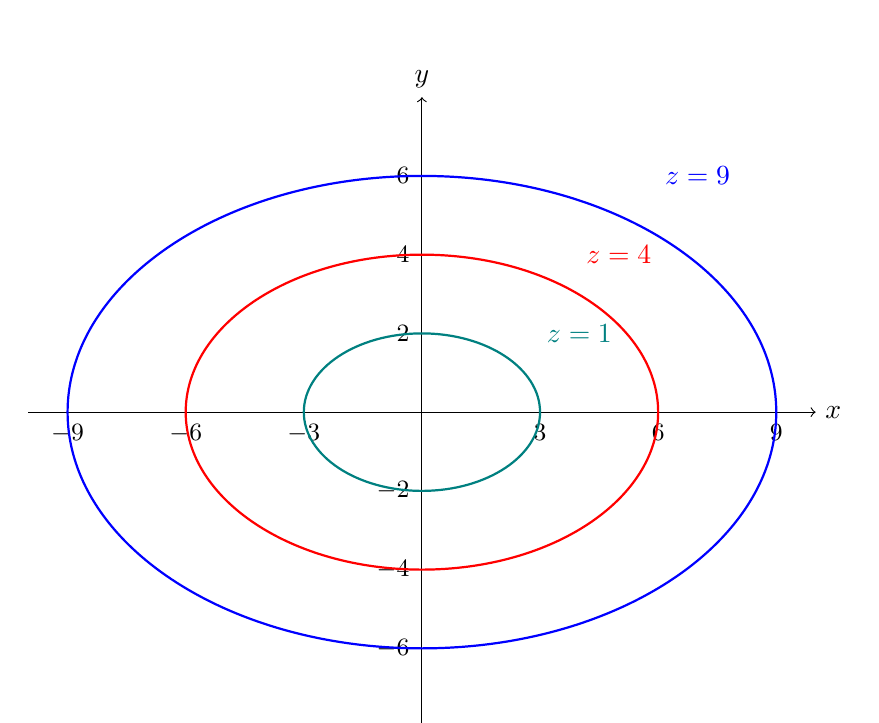
\begin{tikzpicture}[scale=0.5]
            % Ejes
            \draw[->] (-10,0) -- (10,0) node[right] {$x$};
            \draw[->] (0,-8) -- (0,8) node[above] {$y$};
            
            % Ticks en el eje x
            \foreach \x in {-9,-6,-3,3,6,9} {
                \draw[shift={(\x,0)}] (0pt,2pt) -- (0pt,-2pt)
                    node[below] {\small \(\x\)};
            }
            
            % Ticks en el eje y
            \foreach \y in {-6,-4,-2,2,4,6} {
                \draw[shift={(0,\y)}] (2pt,0pt) -- (-2pt,0pt)
                    node[left] {\small \(\y\)};
            }
            
            % Curva para z=1 (elipse de semiejes 3 y 2)
            \draw[teal, thick] (0,0) ellipse (3 and 2);
            \node[teal] at (4,2) {$z=1$};

            % Curva para z=4 (elipse de semiejes 6 y 4)
            \draw[red, thick] (0,0) ellipse (6 and 4);
            \node[red] at (5,4) {$z=4$};

            % Curva para z=9 (elipse de semiejes 9 y 6)
            \draw[blue, thick] (0,0) ellipse (9 and 6);
            \node[blue] at (7,6) {$z=9$};
        \end{tikzpicture}
        \end{center}
        \bigskip
        
        \noindent        
        \textbf{Interpretación en términos de utilidad:} \\
        Si interpretamos \(z\) como una función de utilidad dependiente de los bienes \(x\) e \(y\), las curvas de indiferencia son las elipses mostradas del primer cuadrante. \textbf{\color{teal}Estas no cumplen con la convexidad hacia el origen}




\newpage

%%%%%%%%%%%%%


\subsection{Ejercicio 35}

   Suponga que un consumidor busca maximizar su utilidad que está dada por la siguiente función: $u=x^\alpha y^2$
Donde $\alpha>0$. El precio de $x$ es 2 y el precio de $y$ es 4. El presupuesto disponible es 100.
\begin{enumerate}
    \item Escriba la restricción de este problema de optimización 
    \item Obtenga la solución de $x^*$ e $y^*$. ¿Qué significan estos valores?
    \item Encuentre el valor de $\alpha$ tal que el $x^*=40$
\end{enumerate}


\newpage
\section*{Solución}




        La función de utilidad es
        \[
        u(x,y)=x^\alpha y^2,\quad \alpha>0
        \]
        y el precio de \(x\) es 2, el de \(y\) es 4, con un presupuesto de 100  
        
        \bigskip
        
        \textbf{Restricción presupuestaria:}
        \[
        2x+4y=100
        \]
        
        \bigskip
    
    \textbf{Paso 1: Despejar \(x\) a partir de la función objetivo}
    
    Asumimos que en el óptimo \(x^\alpha y^2=K\). Despejando \(x\) (tomando la raíz positiva),
    \[
    x = \left(\frac{K}{y^2}\right)^{\frac{1}{\alpha}} = K^{\frac{1}{\alpha}}\,y^{-\frac{2}{\alpha}}
    \]
    
    \bigskip
    
    \textbf{Paso 2: Despejar \(x\) a partir de la restricción}
    
    La restricción es
    \[
    2x+4y=100
    \]
    de donde se obtiene:
    \[
    x=\frac{100-4y}{2} = 50-2y
    \]
    
    \bigskip
    
    \textbf{Paso 3: Derivar ambas expresiones respecto a \(y\)}
    
    \underline{De la función objetivo:}  
    Sea
    \[
    x=K^{\frac{1}{\alpha}}\,y^{-\frac{2}{\alpha}}
    \]
    Su derivada con respecto a \(y\) es
    \[
    \frac{dx}{dy} = K^{\frac{1}{\alpha}}\left(-\frac{2}{\alpha}\right)y^{-\frac{2}{\alpha}-1} 
    = -\frac{2}{\alpha}\,K^{\frac{1}{\alpha}}\,y^{-\frac{2}{\alpha}-1}
    \]
    
    \underline{De la restricción:}  
    Para
    \[
    x=50-2y
    \]
    se tiene:
    \[
    \frac{dx}{dy}=-2
    \]
    
    \bigskip
    
    \textbf{Paso 4: Igualar las derivadas}
    
    En el óptimo, las pendientes deben coincidir, por lo que igualamos:
    \[
    -\frac{2}{\alpha}\,K^{\frac{1}{\alpha}}\,y^{-\frac{2}{\alpha}-1}=-2
    \]
    Cancelamos el signo negativo y el factor \(2\):
    \[
    \frac{1}{\alpha}\,K^{\frac{1}{\alpha}}\,y^{-\frac{2}{\alpha}-1}=1
    \]
    Despejamos \(K^{\frac{1}{\alpha}}\):
    \[
    K^{\frac{1}{\alpha}} = \alpha\,y^{\frac{2}{\alpha}+1}
    \]
    Elevando ambos lados a la potencia \(\alpha\):
    \[
    K = \left(\alpha\,y^{\frac{2}{\alpha}+1}\right)^\alpha = \alpha^\alpha\, y^{2+\alpha}
    \]
    
    \bigskip
    \textbf{Paso 5: Despejar \(y\) a partir de la función objetivo y derivar respecto a \(x\)}
    
    Dado que la función de utilidad es
    \[
    u(x,y)=x^\alpha y^2=K
    \]
    despejamos \(y\) (tomando la raíz positiva):
    \[
    y = \left(\frac{K}{x^\alpha}\right)^{\frac{1}{2}} = K^{\frac{1}{2}}\, x^{-\frac{\alpha}{2}}
    \]
    
    Derivamos esta expresión respecto a \(x\):
    \[
    \frac{dy}{dx} = K^{\frac{1}{2}} \cdot \left(-\frac{\alpha}{2}\right)x^{-\frac{\alpha}{2}-1}
    = -\frac{\alpha}{2}\,K^{\frac{1}{2}}\, x^{-\frac{\alpha}{2}-1}
    \]
    
    \bigskip
    \textbf{Paso 6: Despejar \(y\) a partir de la restricción y derivar respecto a \(x\)}
    
    La restricción es:
    \[
    2x + 4y = 100
    \]
    Despejamos \(y\):
    \[
    y = 25 - \frac{x}{2}
    \]
    Por lo tanto, su derivada es
    \[
    \frac{dy}{dx} = -\frac{1}{2}
    \]
    
    \bigskip
    \textbf{Paso 7: Igualar las derivadas obtenidas en ambos despejes respecto a \(x\)}
    
    Igualamos:
    \[
    -\frac{\alpha}{2}\,K^{\frac{1}{2}}\, x^{-\frac{\alpha}{2}-1} \;=\; -\frac{1}{2}
    \]
    Cancelando \(-\frac{1}{2}\) de ambos lados,
    \[
    \frac{\alpha}{2}\,K^{\frac{1}{2}}\, x^{-\frac{\alpha}{2}-1} \;=\; \frac{1}{2}
    \]
    Multiplicamos ambos lados por 2:
    \[
    \alpha\,K^{\frac{1}{2}}\, x^{-\frac{\alpha}{2}-1} \;=\; 1
    \]
    Despejamos \(K^{\frac{1}{2}}\):
    \[
    K^{\frac{1}{2}} = \frac{1}{\alpha}\, x^{\frac{\alpha}{2}+1}
    \]
    Elevando al cuadrado,
    \[
    K = \frac{1}{\alpha^2}\, x^{\alpha+2}
    \]
    
    \bigskip
    \textbf{Paso 8: Igualación de los dos \(K\) obtenidos}
    
    Del proceso inicial (despeje de \(x\) en función de \(y\)) se obtuvo:
    \[
    K_x = \alpha^\alpha\, y^{\alpha+2}
    \]
    Para que ambas igualdades sean consistentes, deben cumplir:
    \[
    \alpha^\alpha\, y^{\alpha+2} \;=\; \frac{1}{\alpha^2}\, x^{\alpha+2}
    \]
    Recordando que, en el punto óptimo, la tangencia implica también la igualdad de pendientes obtenida anteriormente, la relación entre \(x\) y \(y\) resultante es:
    \[ \color{teal}
    x = \alpha\,y
    \]
    
    \bigskip
    \textbf{Paso 9: Determinar \(x^*\) e \(y^*\) utilizando la restricción presupuestaria}
    
    Dado que \(x=\alpha y\) y la restricción es
    \[
    2x+4y=100
    \]
    sustituimos:
    \[
    2(\alpha\,y)+4y = (2\alpha+4)y = 100
    \]
    De aquí,
    \[
    y^* = \frac{100}{2(\alpha+2)} = \frac{50}{\alpha+2}
    \]
    Luego,
    \[
    x^* = \alpha\,y^* = \frac{50\alpha}{\alpha+2}
    \]
    \[
    \color{teal}{x^*=\frac{50\alpha}{\alpha+2} \quad \text{y} \quad y^*=\frac{50}{\alpha+2}}
    \]
    
    \bigskip
    \textbf{Paso 10: Encontrar \(\alpha\) tal que \(x^*=40\)}
    
    Entonces, planteamos la ecuación:
    \[
    \frac{50\alpha}{\alpha+2}=40
    \]
    Multiplicando ambos lados por \(\alpha+2\):
    \[
    50\alpha = 40(\alpha+2)=40\alpha+80
    \]
    Restando \(40\alpha\) de ambos lados:
    \[
    50\alpha-40\alpha=80 \quad\Longrightarrow\quad 10\alpha=80
    \]
    de donde se obtiene:
    \[\color{teal}
    \alpha=8
    \]
    Verificamos:
    \[
    x^*=\frac{50\cdot 8}{8+2}=\frac{400}{10}=40
    \]
    y, de la relación \(y^*=\frac{50}{\alpha+2}\),
    \[
    y^*=\frac{50}{8+2}=\frac{50}{10}=5
    \]
    
    {{\color{teal}\text{Por lo tanto, para } $\alpha=8$ \text{ se tiene } $x^*=40$ \text{ y } $y^*=5$}}


\newpage



    
%%%%%%%%%%%%%%%%%%%%%%%%%%
\section{Derivadas compuestas, derivadas implícitas y homogeneidad}

\subsection{Ejercicio 1}

\subsection*{Calcular las derivadas como funciones compuestas}

\begin{enumerate}
  \item 
  \[
    z = 3x^2 + 4y - 2xy,
    \qquad
    \begin{cases}
      x = t^2 + 1,\\
      y = 2t - 1,
    \end{cases}
    \qquad
    \frac{dz}{dt}
  \]
  
  \item 
  \[
    z = \ln\bigl(x^2 + y^2\bigr),
    \qquad
    \begin{cases}
      x = e^{-t},\\
      y = e^{t},
    \end{cases}
    \qquad
    \frac{dz}{dt}
  \]
  
  \item 
  \[
    z = \frac{2xy}{y^2 + 1},
    \qquad
    \begin{cases}
      x = 2t + 4,\\
      y = 5t^3,
    \end{cases}
    \qquad
    \frac{dz}{dt}
  \]
  
  \item 
  \[
    z = x\,\ln y,
    \qquad
    \begin{cases}
      x = uv,\\
      y = \dfrac{1}{u + v},
    \end{cases}
    \qquad
    \frac{\partial z}{\partial u},\;\frac{\partial z}{\partial v}
  \]

   \item 
  \[
  z = x^3 + y^2 - 2xy,
  \qquad
  \begin{cases}
    x = u + 3uv, \\
    y = v^2 - 3v + uv,
  \end{cases}
  \qquad
  \frac{\partial z}{\partial u}
  \quad\land\quad
  \frac{\partial z}{\partial v}
  \]

  \item 
  \[
  z = \frac{y^3}{\ln x},
  \qquad
  \begin{cases}
    x = \sin u + \ln t, \\
    y = t^u,
  \end{cases}
  \qquad
  \frac{\partial z}{\partial u}
  \quad\land\quad
  \frac{\partial z}{\partial t}
  \]

  \item 
  \[
  z = e^{uv},
  \qquad
  \begin{cases}
    u = \ln(x + y), \\
    v = \operatorname{arctg}\left(\frac{x}{y}\right),
  \end{cases}
  \qquad
  \frac{\partial z}{\partial x}
  \quad\land\quad
  \frac{\partial z}{\partial y}
  \]
\end{enumerate}

\newpage
\section*{Solución}

\subsection*{1)}

Primero hallamos las derivadas parciales:
\[
z_x = \frac{\partial}{\partial x}(3x^2+4y-2xy) = 6x - 2y,
\qquad
z_y = \frac{\partial}{\partial y}(3x^2+4y-2xy) = 4 - 2x.
\]
Luego,
\[
\frac{dx}{dt} = 2t,
\qquad
\frac{dy}{dt} = 2.
\]
Por la regla de la cadena,
\[ \color{teal}
\frac{dz}{dt}
= z_x\,\frac{dx}{dt} + z_y\,\frac{dy}{dt}
= (6x-2y)(2t) + (4-2x)(2).
\]
Sustituyendo \(x=t^2+1\) y \(y=2t-1\):
\[
6x-2y = 6(t^2+1) - 2(2t-1) = 6t^2 -4t +8,
\quad
4-2x = 4 - 2(t^2+1) = 2 - 2t^2,
\]
\[ \color{teal}
\frac{dz}{dt}
= (6t^2 -4t +8)(2t) + (2 - 2t^2)(2)
= 12t^3 -12t^2 +16t +4.
\]

\subsection*{2)}


La regla de la cadena para $\frac{dz}{dt}$ es:
\[
\frac{dz}{dt} = \frac{\partial z}{\partial x} \frac{dx}{dt} + \frac{\partial z}{\partial y} \frac{dy}{dt}
\]

Primero, calculamos las derivadas parciales de $z$ con respecto a $x$ e $y$:
\[
\frac{\partial z}{\partial x} = \frac{1}{x^2 + y^2} \cdot \frac{\partial}{\partial x}(x^2 + y^2) = \frac{1}{x^2 + y^2} \cdot (2x) = \frac{2x}{x^2 + y^2}
\]
\[
\frac{\partial z}{\partial y} = \frac{1}{x^2 + y^2} \cdot \frac{\partial}{\partial y}(x^2 + y^2) = \frac{1}{x^2 + y^2} \cdot (2y) = \frac{2y}{x^2 + y^2}
\]

Luego, calculamos las derivadas de $x$ e $y$ con respecto a $t$:
\[
\frac{dx}{dt} = \frac{d}{dt}(e^{-t}) = -e^{-t}
\]
\[
\frac{dy}{dt} = \frac{d}{dt}(e^{t}) = e^{t}
\]

Ahora, sustituimos estas derivadas en la fórmula de la regla de la cadena:
\[
\frac{dz}{dt} = \left(\frac{2x}{x^2 + y^2}\right)(-e^{-t}) + \left(\frac{2y}{x^2 + y^2}\right)(e^{t})
\]
\[
\frac{dz}{dt} = \frac{-2xe^{-t} + 2ye^{t}}{x^2 + y^2}
\]

Finalmente, sustituimos $x = e^{-t}$ y $y = e^{t}$ en la expresión para $\frac{dz}{dt}$:
\[
\frac{dz}{dt} = \frac{-2(e^{-t})e^{-t} + 2(e^{t})e^{t}}{(e^{-t})^2 + (e^{t})^2}
\]
\[
\frac{dz}{dt} = \frac{-2e^{-2t} + 2e^{2t}}{e^{-2t} + e^{2t}}
\]

Podemos simplificar un poco más factorizando el 2 en el numerador:
\[ \color{teal}
\frac{dz}{dt} = \frac{2(e^{2t} - e^{-2t})}{e^{2t} + e^{-2t}}
\]

\subsection*{3)}
La regla de la cadena para $\frac{dz}{dt}$ es:
\[
\frac{dz}{dt} = \frac{\partial z}{\partial x} \frac{dx}{dt} + \frac{\partial z}{\partial y} \frac{dy}{dt}
\]

Primero, calculamos las derivadas parciales de $z$ con respecto a $x$ e $y$:
\[
\frac{\partial z}{\partial x} = \frac{\partial}{\partial x} \left( \frac{2xy}{y^2 + 1} \right) = \frac{2y}{y^2 + 1} \cdot \frac{\partial}{\partial x}(x) = \frac{2y}{y^2 + 1}
\]
Para $\frac{\partial z}{\partial y}$, usamos la regla del cociente $\left(\frac{u}{v}\right)' = \frac{u'v - uv'}{v^2}$ con $u = 2xy$ y $v = y^2 + 1$.
\[
\frac{\partial u}{\partial y} = 2x, \quad \frac{\partial v}{\partial y} = 2y
\]
\[
\frac{\partial z}{\partial y} = \frac{(2x)(y^2 + 1) - (2xy)(2y)}{(y^2 + 1)^2} = \frac{2xy^2 + 2x - 4xy^2}{(y^2 + 1)^2} = \frac{2x - 2xy^2}{(y^2 + 1)^2} = \frac{2x(1 - y^2)}{(y^2 + 1)^2}
\]

Luego, calculamos las derivadas de $x$ e $y$ con respecto a $t$:
\[
\frac{dx}{dt} = \frac{d}{dt}(2t + 4) = 2
\]
\[
\frac{dy}{dt} = \frac{d}{dt}(5t^3) = 15t^2
\]

Ahora, sustituimos estas derivadas en la fórmula de la regla de la cadena:
\[
\frac{dz}{dt} = \left( \frac{2y}{y^2 + 1} \right) (2) + \left( \frac{2x(1 - y^2)}{(y^2 + 1)^2} \right) (15t^2)
\]
\[ \color{teal}
\frac{dz}{dt} = \frac{4y}{y^2 + 1} + \frac{30xt^2(1 - y^2)}{(y^2 + 1)^2}
\]

Finalmente, sustituimos $x = 2t + 4$ y $y = 5t^3$ en la expresión para $\frac{dz}{dt}$:
\[
y^2 = (5t^3)^2 = 25t^6
\]
\[ \color{teal}
\frac{dz}{dt} = \frac{4(5t^3)}{(5t^3)^2 + 1} + \frac{30(2t + 4)t^2(1 - (5t^3)^2)}{((5t^3)^2 + 1)^2}
\]


\subsection*{4)}
Las reglas de la cadena para las derivadas parciales son:
\[
\frac{\partial z}{\partial u} = \frac{\partial z}{\partial x} \frac{\partial x}{\partial u} + \frac{\partial z}{\partial y} \frac{\partial y}{\partial u}
\]
\[
\frac{\partial z}{\partial v} = \frac{\partial z}{\partial x} \frac{\partial x}{\partial v} + \frac{\partial z}{\partial y} \frac{\partial y}{\partial v}
\]

Primero, calculamos las derivadas parciales de $z$ con respecto a $x$ e $y$:
\[
\frac{\partial z}{\partial x} = \frac{\partial}{\partial x}(x \ln y) = \ln y
\]
\[
\frac{\partial z}{\partial y} = \frac{\partial}{\partial y}(x \ln y) = x \cdot \frac{1}{y} = \frac{x}{y}
\]

Luego, calculamos las derivadas parciales de $x$ e $y$ con respecto a $u$ y $v$:
\[
\frac{\partial x}{\partial u} = \frac{\partial}{\partial u}(uv) = v
\]
\[
\frac{\partial x}{\partial v} = \frac{\partial}{\partial v}(uv) = u
\]
\[
\frac{\partial y}{\partial u} = \frac{\partial}{\partial u}((u+v)^{-1}) = -1(u+v)^{-2} \cdot \frac{\partial}{\partial u}(u+v) = -(u+v)^{-2} \cdot 1 = -\frac{1}{(u+v)^2}
\]
\[
\frac{\partial y}{\partial v} = \frac{\partial}{\partial v}((u+v)^{-1}) = -1(u+v)^{-2} \cdot \frac{\partial}{\partial v}(u+v) = -(u+v)^{-2} \cdot 1 = -\frac{1}{(u+v)^2}
\]

Ahora, sustituimos estas derivadas en las fórmulas de la regla de la cadena.

Para $\frac{\partial z}{\partial u}$:
\[
\frac{\partial z}{\partial u} = (\ln y)(v) + \left(\frac{x}{y}\right)\left(-\frac{1}{(u+v)^2}\right)
\]
Sustituimos $x = uv$ y $y = \frac{1}{u+v}$:
\[
\ln y = \ln\left(\frac{1}{u+v}\right) = \ln((u+v)^{-1}) = -\ln(u+v)
\]
\[
\frac{x}{y} = \frac{uv}{1/(u+v)} = uv(u+v)
\]
Entonces:
\[
\frac{\partial z}{\partial u} = (-\ln(u+v))(v) + (uv(u+v))\left(-\frac{1}{(u+v)^2}\right)
\]
\[
\frac{\partial z}{\partial u} = -v \ln(u+v) - \frac{uv(u+v)}{(u+v)^2}
\]
\[ \color{teal}
{\frac{\partial z}{\partial u} = -v \ln(u+v) - \frac{uv}{u+v}}
\]

Para $\frac{\partial z}{\partial v}$:
\[
\frac{\partial z}{\partial v} = (\ln y)(u) + \left(\frac{x}{y}\right)\left(-\frac{1}{(u+v)^2}\right)
\]
Sustituimos $\ln y = -\ln(u+v)$ y $\frac{x}{y} = uv(u+v)$:
\[
\frac{\partial z}{\partial v} = (-\ln(u+v))(u) + (uv(u+v))\left(-\frac{1}{(u+v)^2}\right)
\]
\[
\frac{\partial z}{\partial v} = -u \ln(u+v) - \frac{uv(u+v)}{(u+v)^2}
\]
\[ \color{teal}
{\frac{\partial z}{\partial v} = -u \ln(u+v) - \frac{uv}{u+v}}
\]



\subsection*{5)}

\paragraph{1. Regla de la Cadena}
Para encontrar $\frac{\partial z}{\partial u}$ y $\frac{\partial z}{\partial v}$, usamos la regla de la cadena para funciones de varias variables:
\[
\frac{\partial z}{\partial u} = \frac{\partial z}{\partial x} \frac{\partial x}{\partial u} + \frac{\partial z}{\partial y} \frac{\partial y}{\partial u}
\]
\[
\frac{\partial z}{\partial v} = \frac{\partial z}{\partial x} \frac{\partial x}{\partial v} + \frac{\partial z}{\partial y} \frac{\partial y}{\partial v}
\]

\paragraph{2. Calcular las derivadas parciales intermedias}
Calculamos las derivadas parciales de $z$ respecto a $x$ e $y$:
\[
\frac{\partial z}{\partial x} = \frac{\partial}{\partial x}(x^3 + y^2 - 2xy) = 3x^2 - 2y
\]
\[
\frac{\partial z}{\partial y} = \frac{\partial}{\partial y}(x^3 + y^2 - 2xy) = 2y - 2x
\]
Calculamos las derivadas parciales de $x$ respecto a $u$ y $v$:
\[
\frac{\partial x}{\partial u} = \frac{\partial}{\partial u}(u + 3uv) = 1 + 3v
\]
\[
\frac{\partial x}{\partial v} = \frac{\partial}{\partial v}(u + 3uv) = 3u
\]
Calculamos las derivadas parciales de $y$ respecto a $u$ y $v$:
\[
\frac{\partial y}{\partial u} = \frac{\partial}{\partial u}(v^2 - 3v + uv) = v
\]
\[
\frac{\partial y}{\partial v} = \frac{\partial}{\partial v}(v^2 - 3v + uv) = 2v - 3 + u
\]

\paragraph{3. Sustituir en las fórmulas de la Regla de la Cadena}
Sustituimos las derivadas calculadas en las fórmulas de la regla de la cadena.

Para $\frac{\partial z}{\partial u}$:
\[
\frac{\partial z}{\partial u} = (3x^2 - 2y) \frac{\partial x}{\partial u} + (2y - 2x) \frac{\partial y}{\partial u}
\]
\[\color{teal}
\frac{\partial z}{\partial u} = (3x^2 - 2y) (1 + 3v) + (2y - 2x) (v)
\]
Para $\frac{\partial z}{\partial v}$:
\[
\frac{\partial z}{\partial v} = (3x^2 - 2y) \frac{\partial x}{\partial v} + (2y - 2x) \frac{\partial y}{\partial v}
\]
\[\color{teal}
\frac{\partial z}{\partial v} = (3x^2 - 2y) (3u) + (2y - 2x) (2v - 3 + u)
\]

\subsection*{6)}


\textbf{Solución:}

Aplicamos la regla de la cadena para funciones de varias variables. Las fórmulas son:
\[
\frac{\partial z}{\partial u} = \frac{\partial z}{\partial x} \frac{\partial x}{\partial u} + \frac{\partial z}{\partial y} \frac{\partial y}{\partial u}
\]
\[
\frac{\partial z}{\partial t} = \frac{\partial z}{\partial x} \frac{\partial x}{\partial t} + \frac{\partial z}{\partial y} \frac{\partial y}{\partial t}
\]

\vspace{1em}

\textbf{Paso 1: Calcular las derivadas parciales intermedias}

Calculamos las derivadas parciales de $z$ con respecto a $x$ e $y$, y las derivadas parciales de $x$ e $y$ con respecto a $u$ y $t$.

\begin{enumerate}
    \item $\displaystyle \frac{\partial z}{\partial x} = \frac{\partial}{\partial x} \left( y^3 (\ln x)^{-1} \right) = y^3 (-1) (\ln x)^{-2} \cdot \frac{1}{x} = -\frac{y^3}{x (\ln x)^2}$

    \item $\displaystyle \frac{\partial z}{\partial y} = \frac{\partial}{\partial y} \left( \frac{y^3}{\ln x} \right) = \frac{3y^2}{\ln x}$

    \item $\displaystyle \frac{\partial x}{\partial u} = \frac{\partial}{\partial u} (\sin u + \ln t) = \cos u$

    \item $\displaystyle \frac{\partial x}{\partial t} = \frac{\partial}{\partial t} (\sin u + \ln t) = \frac{1}{t}$

    \item $\displaystyle \frac{\partial y}{\partial u} = \frac{\partial}{\partial u} (t^u) = t^u \ln t \quad$ (derivada de tipo $a^x$)

    \item $\displaystyle \frac{\partial y}{\partial t} = \frac{\partial}{\partial t} (t^u) = u t^{u-1} \quad$ (derivada de tipo $x^a$)
\end{enumerate}

\vspace{1em}

\textbf{Paso 2: Sustituir en la regla de la cadena}

\textbf{Cálculo de $\frac{\partial z}{\partial u}$:}
\[
\frac{\partial z}{\partial u} = \frac{\partial z}{\partial x} \frac{\partial x}{\partial u} + \frac{\partial z}{\partial y} \frac{\partial y}{\partial u}
\]
\[
\frac{\partial z}{\partial u} = \left( -\frac{y^3}{x (\ln x)^2} \right) (\cos u) + \left( \frac{3y^2}{\ln x} \right) (t^u \ln t)
\]
\[ \color{teal}
\frac{\partial z}{\partial u} = -\frac{y^3 \cos u}{x (\ln x)^2} + \frac{3y^2 t^u \ln t}{\ln x}
\]
Ahora, sustituimos $x = \sin u + \ln t$ y $y = t^u$:
\[
\frac{\partial z}{\partial u} = -\frac{(t^u)^3 \cos u}{(\sin u + \ln t) (\ln(\sin u + \ln t))^2} + \frac{3(t^u)^2 t^u \ln t}{\ln(\sin u + \ln t)}
\]

\vspace{1em}

\textbf{Cálculo de $\frac{\partial z}{\partial t}$:}
\[
\frac{\partial z}{\partial t} = \frac{\partial z}{\partial x} \frac{\partial x}{\partial t} + \frac{\partial z}{\partial y} \frac{\partial y}{\partial t}
\]
\[
\frac{\partial z}{\partial t} = \left( -\frac{y^3}{x (\ln x)^2} \right) \left( \frac{1}{t} \right) + \left( \frac{3y^2}{\ln x} \right) (u t^{u-1})
\]
\[\color{teal}
\frac{\partial z}{\partial t} = -\frac{y^3}{t x (\ln x)^2} + \frac{3y^2 u t^{u-1}}{\ln x}
\]
Sustituyendo $x = \sin u + \ln t$ y $y = t^u$:
\[
\frac{\partial z}{\partial t} = -\frac{(t^u)^3}{t (\sin u + \ln t) (\ln(\sin u + \ln t))^2} + \frac{3(t^u)^2 u t^{u-1}}{\ln(\sin u + \ln t)}
\]

\subsection*{7)}


Aplicamos la regla de la cadena para funciones de varias variables:
\[
\frac{\partial z}{\partial x} = \frac{\partial z}{\partial u} \frac{\partial u}{\partial x} + \frac{\partial z}{\partial v} \frac{\partial v}{\partial x}
\]
\[
\frac{\partial z}{\partial y} = \frac{\partial z}{\partial u} \frac{\partial u}{\partial y} + \frac{\partial z}{\partial v} \frac{\partial v}{\partial y}
\]

\vspace{1em}

\textbf{Paso 1: Calcular las derivadas parciales intermedias}

Calculamos las derivadas parciales de $z$ con respecto a $u$ y $v$, y las derivadas parciales de $u$ y $v$ con respecto a $x$ e $y$.

\begin{enumerate}
    \item $\displaystyle \frac{\partial z}{\partial u} = \frac{\partial}{\partial u} (e^{uv}) = e^{uv} \cdot \frac{\partial}{\partial u}(uv) = e^{uv} \cdot v = v e^{uv}$

    \item $\displaystyle \frac{\partial z}{\partial v} = \frac{\partial}{\partial v} (e^{uv}) = e^{uv} \cdot \frac{\partial}{\partial v}(uv) = e^{uv} \cdot u = u e^{uv}$

    \item $\displaystyle \frac{\partial u}{\partial x} = \frac{\partial}{\partial x} (\ln(x+y)) = \frac{1}{x+y} \cdot \frac{\partial}{\partial x}(x+y) = \frac{1}{x+y} \cdot 1 = \frac{1}{x+y}$

    \item $\displaystyle \frac{\partial u}{\partial y} = \frac{\partial}{\partial y} (\ln(x+y)) = \frac{1}{x+y} \cdot \frac{\partial}{\partial y}(x+y) = \frac{1}{x+y} \cdot 1 = \frac{1}{x+y}$

    \item $\displaystyle \frac{\partial v}{\partial x} = \frac{\partial}{\partial x} \left( \operatorname{arctg}\left(\frac{x}{y}\right) \right) = \frac{1}{1 + \left(\frac{x}{y}\right)^2} \cdot \frac{\partial}{\partial x}\left(\frac{x}{y}\right)$
    \[
    = \frac{1}{1 + \frac{x^2}{y^2}} \cdot \frac{1}{y} = \frac{y^2}{y^2 + x^2} \cdot \frac{1}{y} = \frac{y}{x^2 + y^2}
    \]

    \item $\displaystyle \frac{\partial v}{\partial y} = \frac{\partial}{\partial y} \left( \operatorname{arctg}\left(\frac{x}{y}\right) \right) = \frac{1}{1 + \left(\frac{x}{y}\right)^2} \cdot \frac{\partial}{\partial y}\left(x y^{-1}\right)$
    \[
    = \frac{1}{1 + \frac{x^2}{y^2}} \cdot (x (-1) y^{-2}) = \frac{y^2}{y^2 + x^2} \cdot \left(-\frac{x}{y^2}\right) = -\frac{x}{x^2 + y^2}
    \]
\end{enumerate}

\vspace{1em}

\textbf{Paso 2: Sustituir en la regla de la cadena}

\textbf{Cálculo de $\frac{\partial z}{\partial x}$:}
\[
\frac{\partial z}{\partial x} = \frac{\partial z}{\partial u} \frac{\partial u}{\partial x} + \frac{\partial z}{\partial v} \frac{\partial v}{\partial x}
\]
\[
\frac{\partial z}{\partial x} = (v e^{uv}) \left( \frac{1}{x+y} \right) + (u e^{uv}) \left( \frac{y}{x^2 + y^2} \right)
\]
\[ \color{teal}
\frac{\partial z}{\partial x} = e^{uv} \left( \frac{v}{x+y} + \frac{uy}{x^2 + y^2} \right)
\]
Sustituyendo $u = \ln(x+y)$ y $v = \operatorname{arctg}\left(\frac{x}{y}\right)$:
\[\color{teal}
{
\frac{\partial z}{\partial x} = e^{\ln(x+y) \operatorname{arctg}\left(\frac{x}{y}\right)} \left[ \frac{\operatorname{arctg}\left(\frac{x}{y}\right)}{x+y} + \frac{y \ln(x+y)}{x^2 + y^2} \right]
}
\]

\vspace{1em}

\textbf{Cálculo de $\frac{\partial z}{\partial y}$:}
\[
\frac{\partial z}{\partial y} = \frac{\partial z}{\partial u} \frac{\partial u}{\partial y} + \frac{\partial z}{\partial v} \frac{\partial v}{\partial y}
\]
\[
\frac{\partial z}{\partial y} = (v e^{uv}) \left( \frac{1}{x+y} \right) + (u e^{uv}) \left( -\frac{x}{x^2 + y^2} \right)
\]
\[\color{teal}
\frac{\partial z}{\partial y} = e^{uv} \left( \frac{v}{x+y} - \frac{ux}{x^2 + y^2} \right)
\]
Sustituyendo $u = \ln(x+y)$ y $v = \operatorname{arctg}\left(\frac{x}{y}\right)$:
\[\color{teal}
{
\frac{\partial z}{\partial y} = e^{\ln(x+y) \operatorname{arctg}\left(\frac{x}{y}\right)} \left[ \frac{\operatorname{arctg}\left(\frac{x}{y}\right)}{x+y} - \frac{x \ln(x+y)}{x^2 + y^2} \right]
}
\]

\newpage
\subsection{Ejercicio 2}

Dadas las siguientes ecuaciones, verificar la condición de existencia de las derivadas parciales de 
\(z = f(x,y)\) en el punto indicado. Si existen, hallarlas:

\begin{enumerate}
  \item 
  \(\ln(xy) + z - \sin z + 4y = 4\)
  \hfill en \(P_0 = (1, 1, 0)\)
  
  \item 
  \(e^{xy} - \cos x + 3z^2 - 4z + 1 = 3x\)
  \hfill en \(P_0 = (0, 3, 1)\)
\end{enumerate}

\newpage
\section*{Solución}

\subsection*{1)}

\subsection*{Verificación de las condiciones}

\textbf{Condición 1:} Evaluamos $F$ en el punto $P_0 = (1, 1, 0)$.
\[ F(1, 1, 0) = \ln(1 \cdot 1) + 0 - \sin(0) + 4(1) - 4 \]
\[ F(1, 1, 0) = \ln(1) + 0 - 0 + 4 - 4 \]
\[ F(1, 1, 0) = 0 + 0 - 0 + 0 = 0 \]
La primera condición \textbf{se cumple}, el punto $P_0$ pertenece a la superficie definida por $F(x, y, z) = 0$.

\textbf{Condición 2:} Calculamos las derivadas parciales de $F$ respecto a $x$, $y$, y $z$.
\[ \frac{\partial F}{\partial x} = \frac{\partial}{\partial x} (\ln(xy) + z - \sin z + 4y - 4) = \frac{1}{xy} \cdot y = \frac{1}{x} \]
\[ \frac{\partial F}{\partial y} = \frac{\partial}{\partial y} (\ln(xy) + z - \sin z + 4y - 4) = \frac{1}{xy} \cdot x + 4 = \frac{1}{y} + 4 \]
\[ \frac{\partial F}{\partial z} = \frac{\partial}{\partial z} (\ln(xy) + z - \sin z + 4y - 4) = 1 - \cos z \]

Ahora, evaluamos la derivada parcial respecto a $z$ en el punto $P_0 = (1, 1, 0)$:
\[ \color{teal}\frac{\partial F}{\partial z}(1, 1, 0) = 1 - \cos(0) = 1 - 1 = 0 \]

La segunda condición \textbf{\color{teal} no se cumple}.

\subsection*{2)}


\subsection*{1. Definir la función $F(x, y, z)$}
Reescribimos la ecuación en la forma $F(x, y, z) = 0$:
$$F(x, y, z) = e^{xy} - \cos x + 3z^2 - 4z + 1 - 3x = 0$$

\subsection*{2. Verificar el punto $P_0$}
Sustituimos las coordenadas de $P_0 = (0, 3, 1)$ en $F(x, y, z)$:
$$F(0, 3, 1) = e^{(0)(3)} - \cos(0) + 3(1)^2 - 4(1) + 1 - 3(0)$$
$$F(0, 3, 1) = e^0 - 1 + 3(1) - 4 + 1 - 0$$
$$F(0, 3, 1) = 1 - 1 + 3 - 4 + 1 = 0$$
El punto $P_0$ satisface la ecuación $F(x, y, z) = 0$.

\subsection*{3. Calcular las derivadas parciales de F}
Calculamos $F_x = \frac{\partial F}{\partial x}$, $F_y = \frac{\partial F}{\partial y}$ y $F_z = \frac{\partial F}{\partial z}$:
$$F_x = \frac{\partial}{\partial x} (e^{xy} - \cos x + 3z^2 - 4z + 1 - 3x) = y e^{xy} - (-\sin x) - 3 = y e^{xy} + \sin x - 3$$
$$F_y = \frac{\partial}{\partial y} (e^{xy} - \cos x + 3z^2 - 4z + 1 - 3x) = x e^{xy}$$
$$F_z = \frac{\partial}{\partial z} (e^{xy} - \cos x + 3z^2 - 4z + 1 - 3x) = 6z - 4$$

\subsection*{4. Evaluar las derivadas parciales en $P_0$}
Evaluamos $F_x, F_y, F_z$ en $P_0 = (0, 3, 1)$:
$$F_x(0, 3, 1) = (3) e^{(0)(3)} + \sin(0) - 3 = 3 \cdot e^0 + 0 - 3 = 3 \cdot 1 - 3 = 0$$
$$F_y(0, 3, 1) = (0) e^{(0)(3)} = 0 \cdot 1 = 0$$
$$F_z(0, 3, 1) = 6(1) - 4 = 6 - 4 = 2$$

\subsection*{5. Calcular las derivadas parciales de z}
Utilizamos las fórmulas del Teorema de la Función Implícita:
$$\color{teal}\frac{\partial z}{\partial x} \bigg|_{(0,3)} = - \frac{F_x(0, 3, 1)}{F_z(0, 3, 1)} = - \frac{0}{2} = 0$$
$$\color{teal}\frac{\partial z}{\partial y} \bigg|_{(0,3)} = - \frac{F_y(0, 3, 1)}{F_z(0, 3, 1)} = - \frac{0}{2} = 0$$


\newpage

\subsection{Ejercicio 3}
Calcular las derivadas parciales de las siguientes funciones definidas implícitamente, tales que \(z = f(x,y)\):

\begin{enumerate}
  \item \(x + y + z = \sin(xyz)\)
  \item \(x + 3y + 2z - \ln z = 0\)
  \item \(x^3 + 2y^3 + z^3 - 3xyz - 2y = -3\)
\end{enumerate}


\newpage
\section*{Solución}

\subsection*{1)}
 Para $x + y + z = \sin(xyz)$ donde $z = f(x,y)$:
  
  Si definimos $F(x,y,z) = x + y + z - \sin(xyz) = 0$, entonces:
  
  \begin{equation}\color{teal}
  \frac{\partial z}{\partial x} = -\frac{\frac{\partial F}{\partial x}}{\frac{\partial F}{\partial z}} = -\frac{1 - \cos(xyz) \cdot yz}{1 - \cos(xyz) \cdot xy}
  \end{equation}
  
  \begin{equation} \color{teal}
  \frac{\partial z}{\partial y} = -\frac{\frac{\partial F}{\partial y}}{\frac{\partial F}{\partial z}} = -\frac{1 - \cos(xyz) \cdot xz}{1 - \cos(xyz) \cdot xy}
  \end{equation}


  \subsection*{2)}
Para $x + 3y + 2z - \ln z = 0$ donde $z = f(x,y)$:
  
  Si definimos $F(x,y,z) = x + 3y + 2z - \ln z = 0$, entonces:
  
  \begin{equation} \color{teal}
  \frac{\partial z}{\partial x} = -\frac{\frac{\partial F}{\partial x}}{\frac{\partial F}{\partial z}} = -\frac{1}{2 - \frac{1}{z}}
  \end{equation}
  
  \begin{equation}\color{teal}
  \frac{\partial z}{\partial y} = -\frac{\frac{\partial F}{\partial y}}{\frac{\partial F}{\partial z}} = -\frac{3}{2 - \frac{1}{z}}
  \end{equation}
  \subsection*{3)}

  Para $x^3 + 2y^3 + z^3 - 3xyz - 2y = -3$ donde $z = f(x,y)$:
  
  Si definimos $F(x,y,z) = x^3 + 2y^3 + z^3 - 3xyz - 2y + 3 = 0$, entonces:
  
  \begin{equation}\color{teal}
  \frac{\partial z}{\partial x} = -\frac{\frac{\partial F}{\partial x}}{\frac{\partial F}{\partial z}} = -\frac{3x^2 - 3yz}{3z^2 - 3xy}
  \end{equation}
  
  \begin{equation}\color{teal}
  \frac{\partial z}{\partial y} = -\frac{\frac{\partial F}{\partial y}}{\frac{\partial F}{\partial z}} = -\frac{6y^2 - 3xz - 2}{3z^2 - 3xy}
  \end{equation}

\newpage
\subsection{Ejercicio 4}

Calcular las derivadas parciales segundas de \(z = f(x,y)\) definida implícitamente por:

\begin{enumerate}
  \item \(4x^3 + z^2 y + 3xy^2 = 0\)
  \item \(xyz + e^{xyz} = 0\)
\end{enumerate}



\newpage
\section*{Solución}
\subsection*{1)}

Para $4x^3 + z^2 y + 3xy^2 = 0$ donde $z = f(x,y)$:
  
  Si definimos $F(x,y,z) = 4x^3 + z^2 y + 3xy^2 = 0$, entonces:
  
  Primero calculamos las derivadas parciales primeras:
  \begin{equation} \color{teal}
  \frac{\partial z}{\partial x} = -\frac{\frac{\partial F}{\partial x}}{\frac{\partial F}{\partial z}} = -\frac{12x^2 + 3y^2}{2zy}
  \end{equation}
  
  \begin{equation}\color{teal}
  \frac{\partial z}{\partial y} = -\frac{\frac{\partial F}{\partial y}}{\frac{\partial F}{\partial z}} = -\frac{z^2 + 6xy}{2zy}
  \end{equation}
  
  Ahora calculamos las derivadas segundas. Para $\frac{\partial^2 z}{\partial x^2}$, derivamos $\frac{\partial z}{\partial x}$ respecto a $x$:
  \begin{equation}
  \frac{\partial^2 z}{\partial x^2} = \frac{\partial}{\partial x}\left(-\frac{12x^2 + 3y^2}{2zy}\right)
  \end{equation}
  
  Aplicando la regla del cociente:
  \begin{equation}
  \frac{\partial^2 z}{\partial x^2} = -\frac{(2zy)\frac{\partial}{\partial x}(12x^2 + 3y^2) - (12x^2 + 3y^2)\frac{\partial}{\partial x}(2zy)}{(2zy)^2}
  \end{equation}
  
  \begin{equation}\color{teal}
  \frac{\partial^2 z}{\partial x^2} = -\frac{(2zy)(24x) - (12x^2 + 3y^2)(2y\frac{\partial z}{\partial x})}{4z^2y^2}
  \end{equation}
  
  Sustituyendo $\frac{\partial z}{\partial x}$:
  \begin{equation}\color{teal}
  \frac{\partial^2 z}{\partial x^2} = -\frac{(2zy)(24x) - (12x^2 + 3y^2)(2y)(-\frac{12x^2 + 3y^2}{2zy})}{4z^2y^2}
  \end{equation}
  
  
  Para $\frac{\partial^2 z}{\partial y^2}$, derivamos $\frac{\partial z}{\partial y}$ respecto a $y$:
  \begin{equation}
  \frac{\partial^2 z}{\partial y^2} = \frac{\partial}{\partial y}\left(-\frac{z^2 + 6xy}{2zy}\right)
  \end{equation}
  
  Aplicando la regla del cociente:
  \begin{equation}
  \frac{\partial^2 z}{\partial y^2} = -\frac{(2zy)\frac{\partial}{\partial y}(z^2 + 6xy) - (z^2 + 6xy)\frac{\partial}{\partial y}(2zy)}{(2zy)^2}
  \end{equation}
  
  \begin{equation}\color{teal}
  \frac{\partial^2 z}{\partial y^2} = -\frac{(2zy)(2z\frac{\partial z}{\partial y} + 6x) - (z^2 + 6xy)(2z + 2y\frac{\partial z}{\partial y})}{4z^2y^2}
  \end{equation}
  
  Sustituyendo $\frac{\partial z}{\partial y}$:
  \begin{equation}\color{teal}
  \frac{\partial^2 z}{\partial y^2} = -\frac{(2zy)(2z)(-\frac{z^2 + 6xy}{2zy}) + (2zy)(6x) - (z^2 + 6xy)(2z + 2y)(-\frac{z^2 + 6xy}{2zy})}{4z^2y^2}
  \end{equation}
  
  Para $\frac{\partial^2 z}{\partial x \partial y}$, derivamos $\frac{\partial z}{\partial x}$ respecto a $y$:
  \begin{equation}
  \frac{\partial^2 z}{\partial x \partial y} = \frac{\partial}{\partial y}\left(-\frac{12x^2 + 3y^2}{2zy}\right)
  \end{equation}
  
  Aplicando la regla del cociente:
  \begin{equation}
  \frac{\partial^2 z}{\partial x \partial y} = -\frac{(2zy)\frac{\partial}{\partial y}(12x^2 + 3y^2) - (12x^2 + 3y^2)\frac{\partial}{\partial y}(2zy)}{(2zy)^2}
  \end{equation}
  
  \begin{equation}\color{teal}
  \frac{\partial^2 z}{\partial x \partial y} = -\frac{(2zy)(6y) - (12x^2 + 3y^2)(2z + 2y\frac{\partial z}{\partial y})}{4z^2y^2}
  \end{equation}
  
  Sustituyendo $\frac{\partial z}{\partial y}$:
  \begin{equation}\color{teal}
  \frac{\partial^2 z}{\partial x \partial y} = -\frac{(2zy)(6y) - (12x^2 + 3y^2)(2z + 2y)(-\frac{z^2 + 6xy}{2zy})}{4z^2y^2}
  \end{equation}

\subsection*{2)}
Para $xyz + e^{xyz} = 0$ donde $z = f(x,y)$:
  
  Si definimos $F(x,y,z) = xyz + e^{xyz} = 0$, entonces:
  
  Primero calculamos las derivadas parciales de $F$:
  \begin{align}
  \frac{\partial F}{\partial x} &= yz + yz \cdot e^{xyz} \\
  \frac{\partial F}{\partial y} &= xz + xz \cdot e^{xyz} \\
  \frac{\partial F}{\partial z} &= xy + xy \cdot e^{xyz}
  \end{align}
  
  Obtenemos las derivadas parciales primeras:
  \begin{equation}
  \frac{\partial z}{\partial x} = -\frac{\frac{\partial F}{\partial x}}{\frac{\partial F}{\partial z}} = -\frac{yz + yz \cdot e^{xyz}}{xy + xy \cdot e^{xyz}} = -\frac{yz(1 + e^{xyz})}{xy(1 + e^{xyz})} = \color{teal} -\frac{z}{x}
  \end{equation}
  
  \begin{equation}
  \frac{\partial z}{\partial y} = -\frac{\frac{\partial F}{\partial y}}{\frac{\partial F}{\partial z}} = -\frac{xz + xz \cdot e^{xyz}}{xy + xy \cdot e^{xyz}} = -\frac{xz(1 + e^{xyz})}{xy(1 + e^{xyz})} = \color{teal}-\frac{z}{y}
  \end{equation}
  
  Ahora calculamos las derivadas parciales segundas:
  
  Para $\frac{\partial^2 z}{\partial x^2}$, derivamos $\frac{\partial z}{\partial x} = -\frac{z}{x}$ respecto a $x$:
  \begin{equation}\color{teal}
  \frac{\partial^2 z}{\partial x^2} = -\frac{x \cdot \frac{\partial z}{\partial x} - z \cdot 1}{x^2} = -\frac{x \cdot (-\frac{z}{x}) - z}{x^2} = -\frac{z + z}{x^2} = -\frac{2z}{x^2}
  \end{equation}
  
  Para $\frac{\partial^2 z}{\partial y^2}$, derivamos $\frac{\partial z}{\partial y} = -\frac{z}{y}$ respecto a $y$:
  \begin{equation}\color{teal}
  \frac{\partial^2 z}{\partial y^2} = -\frac{y \cdot \frac{\partial z}{\partial y} - z \cdot 1}{y^2} = -\frac{y \cdot (-\frac{z}{y}) - z}{y^2} = -\frac{z + z}{y^2} = -\frac{2z}{y^2}
  \end{equation}
  
  Para $\frac{\partial^2 z}{\partial x \partial y}$, derivamos $\frac{\partial z}{\partial x} = -\frac{z}{x}$ respecto a $y$:
  \begin{equation}\color{teal}
  \frac{\partial^2 z}{\partial x \partial y} = -\frac{1}{x} \cdot \frac{\partial z}{\partial y} = -\frac{1}{x} \cdot \left(-\frac{z}{y}\right) = \frac{z}{xy}
  \end{equation}
  

\newpage
\subsection{Ejercicio 5}
Calcular las derivadas pedidas de las funciones definidas implícitamente por los siguientes sistemas de ecuaciones:

\begin{enumerate}
  \item
    \[
    \begin{cases}
      x^3 + 2y^3 - 3z - 13 = 0\\[4pt]
      x - 6y + z^3 + 5 = 0
    \end{cases}
    \qquad
    \frac{dy}{dx},\quad \frac{dz}{dx}
    \]
  \item
    \[
    \begin{cases}
      x + y - u - v = 0\\[4pt]
      x\,u + y\,v - 1 = 0
    \end{cases}
    \qquad
    \frac{\partial u}{\partial x},\quad \frac{\partial u}{\partial y}
    \quad\text{y}\quad
    \frac{\partial v}{\partial x},\quad \frac{\partial v}{\partial y}
    \]
  \item
    \[
    \begin{cases}
      x^2 - y^2 - u^3 + v^2 + 4 = 0\\[4pt]
      2xy + y^2 - 2u^2 + 3v^4 + 8 = 0
    \end{cases}
    \qquad
    \frac{\partial u}{\partial x},\quad \frac{\partial u}{\partial y}
    \quad\text{y}\quad
    \frac{\partial v}{\partial x},\quad \frac{\partial v}{\partial y}
    \]
\end{enumerate}

\newpage
\section*{Solución}

\subsection*{a)}

Sea el sistema
\[
\begin{cases}
F(x,y,z) = x^3 + 2y^3 - 3z - 13 = 0\\[4pt]
G(x,y,z) = x - 6y + z^3 + 5 = 0
\end{cases}
\]
definiendo \(y = y(x)\) y \(z = z(x)\). Al derivar implícitamente respecto a \(x\) obtenemos
\[
F_x + F_y\,y' + F_z\,z' = 0
\qquad
G_x + G_y\,y' + G_z\,z' = 0
\]
donde
\[
\begin{aligned}
F_x &= 3x^2 &\qquad F_y &= 6y^2 &\qquad F_z &= -3\\
G_x &= 1    &\qquad G_y &= -6   &\qquad G_z &= 3z^2
\end{aligned}
\]
Escribimos en forma matricial:
\[
\begin{pmatrix}
F_y & F_z\\
G_y & G_z
\end{pmatrix}
\begin{pmatrix}
y'\\
z'
\end{pmatrix}
=
-
\begin{pmatrix}
F_x\\
G_x
\end{pmatrix}
\]
El determinante del Jacobiano es
\[
\Delta
= \det
\begin{pmatrix}
6y^2 & -3\\
-6   & 3z^2
\end{pmatrix}
= 18(y^2z^2-1)
\]
Por Cramer:
\[
\color{teal}
y'
=\frac{\det\begin{pmatrix} -F_x & F_z\\ -G_x & G_z \end{pmatrix}}{\Delta}
=\frac{\det\begin{pmatrix} -3x^2 & -3\\ -1 & 3z^2 \end{pmatrix}}{18(y^2z^2-1)}
=-\frac{9x^2z^2+3}{18(y^2z^2-1)}
=-\frac{3x^2z^2+1}{6(y^2z^2-1)}
\]
\[
\color{teal}
z'
=\frac{\det\begin{pmatrix} F_y & -F_x\\ G_y & -G_x \end{pmatrix}}{\Delta}
=\frac{\det\begin{pmatrix} 6y^2 & -3x^2\\ -6 & -1 \end{pmatrix}}{18(y^2z^2-1)}
=-\frac{6y^2+18x^2}{18(y^2z^2-1)}
=-\frac{y^2+3x^2}{3(y^2z^2-1)}
\]

\subsection*{b)}

Sea el sistema
\[
\begin{cases}
F(x,y,u,v) = x + y - u - v = 0\\[4pt]
G(x,y,u,v) = x\,u + y\,v - 1 = 0
\end{cases}
\]
que define \(u = u(x,y)\) y \(v = v(x,y)\). Al diferenciar implícitamente obtenemos el sistema lineal
\[
\begin{pmatrix}
F_u & F_v\\
G_u & G_v
\end{pmatrix}
\begin{pmatrix}
u_x\\
v_x
\end{pmatrix}
=
-
\begin{pmatrix}
F_x\\
G_x
\end{pmatrix}
\qquad
\begin{pmatrix}
F_u & F_v\\
G_u & G_v
\end{pmatrix}
\begin{pmatrix}
u_y\\
v_y
\end{pmatrix}
=
-
\begin{pmatrix}
F_y\\
G_y
\end{pmatrix}
\]
Calculamos las derivadas parciales:
\[
F_u = -1
\qquad
F_v = -1
\qquad
F_x = 1
\qquad
F_y = 1
\]
\[
G_u = x
\qquad
G_v = y
\qquad
G_x = u
\qquad
G_y = v
\]
El determinante común es
\[
\Delta
= \det
\begin{pmatrix}
-1 & -1\\
x  & y
\end{pmatrix}
= x - y
\]
Por Cramer:
\[
\color{teal}
u_x
=\frac{\det\begin{pmatrix} -F_x & F_v\\ -G_x & G_v \end{pmatrix}}{\Delta}
=\frac{\det\begin{pmatrix} -1 & -1\\ -u & y \end{pmatrix}}{x-y}
=\frac{-1\cdot y -(-1)(-u)}{x-y}
=-\frac{u+y}{x-y}
\]
\[
\color{teal}
v_x
=\frac{\det\begin{pmatrix} F_u & -F_x\\ G_u & -G_x \end{pmatrix}}{\Delta}
=\frac{\det\begin{pmatrix} -1 & -1\\ x & -u \end{pmatrix}}{x-y}
=\frac{-1\cdot(-u)-(-1)x}{x-y}
=\frac{u+x}{x-y}
\]
\[
\color{teal}
u_y
=\frac{\det\begin{pmatrix} -F_y & F_v\\ -G_y & G_v \end{pmatrix}}{\Delta}
=\frac{\det\begin{pmatrix} -1 & -1\\ -v & y \end{pmatrix}}{x-y}
=\frac{-y - v}{x-y}
=-\frac{v+y}{x-y}
\]
\[
\color{teal}
v_y
=\frac{\det\begin{pmatrix} F_u & -F_y\\ G_u & -G_y \end{pmatrix}}{\Delta}
=\frac{\det\begin{pmatrix} -1 & -1\\ x & -v \end{pmatrix}}{x-y}
=\frac{-1\cdot(-v)-(-1)x}{x-y}
=\frac{v+x}{x-y}
\]

\subsection*{c)}

Sea
\[
\begin{cases}
F(x,y,u,v)=x^2 - y^2 - u^3 + v^2 + 4 = 0\\[4pt]
G(x,y,u,v)=2xy + y^2 - 2u^2 + 3v^4 + 8 = 0
\end{cases}
\]
definiendo \(u = u(x,y)\) y \(v = v(x,y)\). Al derivar implícitamente respecto a \(x\) obtenemos
\[
F_x + F_u\,u_x + F_v\,v_x = 0
\qquad
G_x + G_u\,u_x + G_v\,v_x = 0
\]
donde
\[
\begin{aligned}
F_x &= 2x &\qquad F_u &= -3u^2 &\qquad F_v &= 2v\\
G_x &= 2y &\qquad G_u &= -4u   &\qquad G_v &= 12v^3
\end{aligned}
\]
En forma matricial:
\[
\begin{pmatrix}
F_u & F_v\\
G_u & G_v
\end{pmatrix}
\begin{pmatrix}
u_x\\
v_x
\end{pmatrix}
=
-\begin{pmatrix}
F_x\\
G_x
\end{pmatrix}
\]
El determinante común es
\[
\Delta
= \det
\begin{pmatrix}
F_u & F_v\\
G_u & G_v
\end{pmatrix}
= (-3u^2)(12v^3) - (2v)(-4u)
= -36u^2v^3 + 8uv
\]
Por Cramer:
\[
\color{teal}
u_x
=\frac{\det\begin{pmatrix} -F_x & F_v\\ -G_x & G_v \end{pmatrix}}{\Delta}
=\frac{(-2x)(12v^3) - (2v)(-2y)}{-36u^2v^3+8uv}
=\frac{-24xv^3 + 4yv}{-36u^2v^3+8uv}
\]
\[
\color{teal}
v_x
=\frac{\det\begin{pmatrix} F_u & -F_x\\ G_u & -G_x \end{pmatrix}}{\Delta}
=\frac{(-3u^2)(-2y) - (-2x)(-4u)}{-36u^2v^3+8uv}
=\frac{6u^2y - 8xu}{-36u^2v^3+8uv}
\]

Análogamente, al derivar respecto a \(y\):
\[
F_y + F_u\,u_y + F_v\,v_y = 0
\qquad
G_y + G_u\,u_y + G_v\,v_y = 0
\]
con
\[
F_y = -2y
\qquad
G_y = 2x + 2y
\]
Por Cramer:
\[
\color{teal}
u_y
=\frac{\det\begin{pmatrix} -F_y & F_v\\ -G_y & G_v \end{pmatrix}}{\Delta}
=\frac{(2y)(12v^3) - (2v)(2x+2y)}{-36u^2v^3+8uv}
=\frac{24yv^3 + 4v(x+y)}{-36u^2v^3+8uv}
\]
\[
\color{teal}
v_y
=\frac{\det\begin{pmatrix} F_u & -F_y\\ G_u & -G_y \end{pmatrix}}{\Delta}
=\frac{(-3u^2)(-(2x+2y)) - (2y)(-4u)}{-36u^2v^3+8uv}
=\frac{6u^2(x+y) + 8uy}{-36u^2v^3+8uv}
\]


\newpage


\subsection{Ejercicio 6}

Indicar si las siguientes funciones son homogéneas y, en caso de que lo sean, indicar el grado.  
Para las funciones que sean homogéneas, verificar el teorema de Euler.

\begin{enumerate}
  \item \(f(x,y) = 3x^2 + 5y - y^2\)
  \item \(f(x,y) = \sqrt{2x^2 + y^2}\)
  \item \(f(x,y) = x^2\,e^{\frac{3}{y^2}}\)
  \item \(f(x,y) = \cos\left(\frac{x}{y}\right)\)
\end{enumerate}

\newpage
\section*{Solución}

\subsection*{1)}

Para \(f(x,y) = 3x^2 + 5y - y^2\):

Una función \(f(x,y)\) es homogénea de grado \(n\) si \(f(tx,ty) = t^n f(x,y)\) para todo \(t > 0\)

Evaluamos \(f(tx,ty)\):
\[
f(tx,ty) = 3(tx)^2 + 5(ty) - (ty)^2
\]
\[
= 3t^2x^2 + 5ty - t^2y^2
\]

Observamos que:
\[
\color{teal}
f(tx,ty) = 3t^2x^2 + 5ty - t^2y^2
= t^2(3x^2 - y^2) + t(5y)
\]

\textbf{\color{teal}Como tenemos términos con distintos exponentes de \(t\) (\(t^1\) y \(t^2\)), no podemos factorizar un \(t^n\) común. Por lo tanto, la función \(f(x,y) = 3x^2 + 5y - y^2\) no es homogénea}

\textbf{\color{teal}Al no ser homogénea, no podemos aplicar el teorema de Euler para esta función}

\subsection*{2)}

Para \(f(x,y) = \sqrt{2x^2 + y^2}\):

Una función \(f(x,y)\) es homogénea de grado \(n\) si \(f(tx,ty) = t^n f(x,y)\) para todo \(t > 0\)

Evaluamos \(f(tx,ty)\):
\[
f(tx,ty) = \sqrt{2(tx)^2 + (ty)^2}
\]
\[
= \sqrt{2t^2x^2 + t^2y^2}
\]
\[
= \sqrt{t^2(2x^2 + y^2)}
\]
\[
= t\sqrt{2x^2 + y^2}
\]
\[
\color{teal}
= t \cdot f(x,y)
\]

\textbf{\color{teal}Como \(f(tx,ty) = t^1 \cdot f(x,y)\), la función \(f(x,y) = \sqrt{2x^2 + y^2}\) es homogénea de grado \(n = 1\)}

\textbf{Verificación del teorema de Euler:}

El teorema de Euler establece que si \(f(x,y)\) es homogénea de grado \(n\), entonces:
\[
x\frac{\partial f}{\partial x} + y\frac{\partial f}{\partial y} = n \cdot f(x,y)
\]

Calculamos las derivadas parciales:

\[
\frac{\partial f}{\partial x} = \frac{1}{2}(2x^2 + y^2)^{-\frac{1}{2}} \cdot 4x = \frac{2x}{\sqrt{2x^2 + y^2}}
\]

\[
\frac{\partial f}{\partial y} = \frac{1}{2}(2x^2 + y^2)^{-\frac{1}{2}} \cdot 2y = \frac{y}{\sqrt{2x^2 + y^2}}
\]

Ahora, evaluamos la expresión del teorema de Euler:
\[
\color{teal}
x\frac{\partial f}{\partial x} + y\frac{\partial f}{\partial y}
= x \cdot \frac{2x}{\sqrt{2x^2 + y^2}} + y \cdot \frac{y}{\sqrt{2x^2 + y^2}}
= \frac{2x^2 + y^2}{\sqrt{2x^2 + y^2}}
= \sqrt{2x^2 + y^2}
= f(x,y)
\]

Como
\[
x\frac{\partial f}{\partial x} + y\frac{\partial f}{\partial y} = 1\cdot f(x,y)
\]
y \(n = 1\), se verifica el teorema de Euler
\subsection*{3)}

Para \(f(x,y) = x^2\,e^{\frac{3}{y^2}}\):

Una función \(f(x,y)\) es homogénea de grado \(n\) si \(f(tx,ty) = t^n f(x,y)\) para todo \(t > 0\)

Evaluamos \(f(tx,ty)\):
\[
f(tx,ty) = (tx)^2\,e^{\frac{3}{(ty)^2}}
\]
\[
= t^2x^2\,e^{\frac{3}{t^2y^2}}
\]
\[
= t^2x^2\,e^{\frac{3}{y^2} \cdot \frac{1}{t^2}}
\]

Observamos que no podemos expresar esto como \(t^n f(x,y)\) debido al término exponencial, ya que:
\[
\color{teal}
e^{\frac{3}{y^2} \cdot \frac{1}{t^2}} \neq t^k \cdot e^{\frac{3}{y^2}}
\]
para ningún valor de \(k\)

\textbf{\color{teal}Por lo tanto, la función \(f(x,y) = x^2\,e^{\frac{3}{y^2}}\) no es homogénea}

\textbf{\color{teal}Al no ser homogénea, no podemos aplicar el teorema de Euler para esta función}

\subsection*{4)}

Para \(f(x,y) = \cos\left(\frac{x}{y}\right)\):

Evaluamos \(f(tx,ty)\):
\[
f(tx,ty) = \cos\left(\frac{tx}{ty}\right)
\]
\[
= \cos\left(\frac{x}{y} \cdot \frac{t}{t}\right)
\]
\[
= \cos\left(\frac{x}{y}\right)
\]
\[
\color{teal}
= f(x,y)
\]

Observamos que \(f(tx,ty) = f(x,y)\), lo que equivale a decir que \(f(tx,ty) = t^0 f(x,y)\)

\textbf{\color{teal}Por lo tanto, la función \(f(x,y) = \cos\left(\frac{x}{y}\right)\) es homogénea de grado 0}

\subsection*{Verificación del teorema de Euler}

Para una función homogénea \(f(x,y)\) de grado \(k\), el teorema de Euler establece que:
\[
x\frac{\partial f}{\partial x} + y\frac{\partial f}{\partial y} = k \cdot f(x,y)
\]

Calculamos las derivadas parciales:
\[
\frac{\partial f}{\partial x} = -\sin\left(\frac{x}{y}\right) \cdot \frac{1}{y}
\]
\[
\frac{\partial f}{\partial y} = -\sin\left(\frac{x}{y}\right) \cdot \left(-\frac{x}{y^2}\right) = \sin\left(\frac{x}{y}\right) \cdot \frac{x}{y^2}
\]

Ahora verificamos el teorema de Euler:
\[
x\frac{\partial f}{\partial x} + y\frac{\partial f}{\partial y}
= x \cdot \left(-\sin\left(\frac{x}{y}\right) \cdot \frac{1}{y}\right) + y \cdot \left(\sin\left(\frac{x}{y}\right) \cdot \frac{x}{y^2}\right)
\]
\[
= -\frac{x}{y}\sin\left(\frac{x}{y}\right) + \frac{x}{y}\sin\left(\frac{x}{y}\right)
\]
\[
\color{teal}
= 0
\]

\textbf{\color{teal}La función \(f(x,y) = \cos\left(\frac{x}{y}\right)\) es homogénea de grado 0 y satisface el teorema de Euler}


\newpage
\subsection{Ejercicio 7}
La función de demanda de un bien está dada por
\[
D_1 = 1000 - 2p_1^2 + 4p_2^3 - 3p_2p_3^2
\]
donde la evolución de los precios respecto del tiempo sigue las leyes
\[
p_1 = 2 + 3t
\qquad
p_2 = 3 + t^2
\qquad
p_3 = t + t^3
\]

Calcular la demanda marginal respecto del tiempo cuando \(t = 1\)  
Interpretar económicamente el resultado

\newpage
\section*{Solución}

La demanda marginal respecto del tiempo es la derivada de \(D_1\) con respecto a \(t\), es decir, \(\frac{dD_1}{dt}\)

Aplicamos la regla de la cadena:
\[
\frac{dD_1}{dt} = \frac{\partial D_1}{\partial p_1} \cdot \frac{dp_1}{dt} + \frac{\partial D_1}{\partial p_2} \cdot \frac{dp_2}{dt} + \frac{\partial D_1}{\partial p_3} \cdot \frac{dp_3}{dt}
\]

Calculamos cada término:

\[
\frac{\partial D_1}{\partial p_1} = -4p_1
\]
\[
\frac{\partial D_1}{\partial p_2} = 12p_2^2 - 3p_3^2
\]
\[
\frac{\partial D_1}{\partial p_3} = -6p_2p_3
\]
\[
\frac{dp_1}{dt} = 3
\]
\[
\frac{dp_2}{dt} = 2t
\]
\[
\frac{dp_3}{dt} = 1 + 3t^2
\]

Sustituimos en la fórmula de la regla de la cadena:

\[
\frac{dD_1}{dt} = (-4p_1)(3) + (12p_2^2 - 3p_3^2)(2t) + (-6p_2p_3)(1 + 3t^2)
\]
\[
\color{teal}
= -12p_1 + (24t)p_2^2 - (6t)p_3^2 - 6p_2p_3 - 18t^2p_2p_3
\]

Evaluamos cuando \(t = 1\):

\[
p_1(1) = 2 + 3(1) = 5
\]
\[
p_2(1) = 3 + 1^2 = 4
\]
\[
p_3(1) = 1 + 1^3 = 2
\]

Sustituimos estos valores:

\[
\color{teal}
\frac{dD_1}{dt}\Big|_{t=1} = -12 \cdot 5 + 24 \cdot 1 \cdot 4^2 - 6 \cdot 1 \cdot 2^2 - 6 \cdot 4 \cdot 2 - 18 \cdot 1^2 \cdot 4 \cdot 2
\]
\[
\color{teal}
= 108
\]

\bigskip

\textbf{\color{teal}Interpretación económica:}

\textbf{\color{teal}La demanda marginal de 108 unidades por unidad de tiempo significa que cuando \(t = 1\), la demanda del bien está aumentando a razón de 108 unidades por cada unidad adicional de tiempo. Este valor positivo indica que la demanda está creciendo.}


\newpage
\subsection{Ejercicio 8}

La demanda de cebada en una determinada población fue estimada para un período según la ley
\[
D_c = \frac{100}{p_c} + p_m^2
\]
donde \(p_c\) es el precio de la cebada y \(p_m\) es el precio del maíz

Si, además, la demanda del maíz fue estimada por la ley
\[
D_m = 8p_c - 3p_m + 100
\]
se pide:

\begin{enumerate}
  \item Indicar si ambos bienes son típicos
  \item Clasificar ambos bienes entre sí
  \item Si la función ingreso está dada por 
  \[
  I = 25\,D_c + 20\,D_m
  \]
  calcular el ingreso marginal respecto del precio de la cebada y respecto del precio del maíz
\end{enumerate}

\newpage
\section*{Solución}

\subsection*{1)}

Un bien es típico cuando la demanda disminuye al aumentar su propio precio, es decir, cuando la derivada parcial de la demanda respecto a su propio precio es negativa

Para la cebada:
\[
\frac{\partial D_c}{\partial p_c} = \frac{\partial}{\partial p_c}\left(\frac{100}{p_c} + p_m^2\right)
\]
\[
\color{teal}
= -\frac{100}{p_c^2}
\]

\textbf{\color{teal}Como \(p_c > 0\) (precios positivos), entonces \(-\frac{100}{p_c^2} < 0\). Por lo tanto, la cebada es un bien típico}

Para el maíz:
\[
\frac{\partial D_m}{\partial p_m} = \frac{\partial}{\partial p_m}(8p_c - 3p_m + 100)
\]
\[
\color{teal}
= -3
\]

\textbf{\color{teal}Como \(-3 < 0\), el maíz también es un bien típico}

\subsection*{2) Clasificar ambos bienes entre sí}

La clasificación de los bienes entre sí depende de cómo la demanda de un bien responde a cambios en el precio del otro bien:

\begin{itemize}
  \item Si \(\frac{\partial D_i}{\partial p_j} > 0\), los bienes \(i\) y \(j\) son sustitutos
  \item Si \(\frac{\partial D_i}{\partial p_j} < 0\), los bienes \(i\) y \(j\) son complementarios
  \item Si \(\frac{\partial D_i}{\partial p_j} = 0\), los bienes \(i\) y \(j\) son independientes
\end{itemize}

Calculemos:

\[
\frac{\partial D_c}{\partial p_m} = \frac{\partial}{\partial p_m}\left(\frac{100}{p_c} + p_m^2\right)
\]
\[
\color{teal}
= 2p_m
\]

\textbf{\color{teal}Como \(p_m > 0\) (precios positivos), entonces \(2p_m > 0\). Esto indica que cuando aumenta el precio del maíz, aumenta la demanda de cebada, lo que sugiere que son bienes sustitutos desde la perspectiva de la cebada}

Por otro lado:

\[
\frac{\partial D_m}{\partial p_c} = \frac{\partial}{\partial p_c}(8p_c - 3p_m + 100)
\]
\[
\color{teal}
= 8
\]

\textbf{\color{teal}Como \(8 > 0\), cuando aumenta el precio de la cebada, aumenta la demanda del maíz, confirmando que los bienes son sustitutos también desde la perspectiva del maíz}
\subsection*{3)}

La función ingreso está dada por:
\[
I = 25\,D_c + 20\,D_m
\]

donde:
\[
D_c = \frac{100}{p_c} + p_m^2
\]
\[
D_m = 8p_c - 3p_m + 100
\]

\textbf{Aplicando la regla de la cadena:}

Para calcular el ingreso marginal respecto a \(p_c\) (precio de la cebada):

\[
\frac{\partial I}{\partial p_c} = \frac{\partial I}{\partial D_c} \cdot \frac{\partial D_c}{\partial p_c} + \frac{\partial I}{\partial D_m} \cdot \frac{\partial D_m}{\partial p_c}
\]
\[
= 25 \cdot \left(-\frac{100}{p_c^2}\right) + 20 \cdot 8
\]
\[
\color{teal}
= -\frac{2500}{p_c^2} + 160
\]

Para calcular el ingreso marginal respecto a \(p_m\) (precio del maíz):

\[
\frac{\partial I}{\partial p_m} = \frac{\partial I}{\partial D_c} \cdot \frac{\partial D_c}{\partial p_m} + \frac{\partial I}{\partial D_m} \cdot \frac{\partial D_m}{\partial p_m}
\]
\[
= 25 \cdot (2p_m) + 20 \cdot (-3)
\]
\[
\color{teal}
= 50p_m - 60
\]

\textbf{Donde hemos usado:}
\[
\frac{\partial I}{\partial D_c} = 25
\]
\[
\frac{\partial I}{\partial D_m} = 20
\]
\[
\frac{\partial D_c}{\partial p_c} = -\frac{100}{p_c^2}
\]
\[
\frac{\partial D_c}{\partial p_m} = 2p_m
\]
\[
\frac{\partial D_m}{\partial p_c} = 8
\]
\[
\frac{\partial D_m}{\partial p_m} = -3
\]

\textbf{Por lo tanto:}
\begin{itemize}
    \item El ingreso marginal respecto del precio de la cebada es: \(\color{teal} \frac{\partial I}{\partial p_c} = -\frac{2500}{p_c^2} + 160\)
    \item El ingreso marginal respecto del precio del maíz es: \(\color{teal} \frac{\partial I}{\partial p_m} = 50p_m - 60\)
\end{itemize}

\textbf{\color{teal}Interpretación económica:}

\textbf{\color{teal}El ingreso marginal respecto a cada precio muestra cómo cambia el ingreso total ante pequeñas variaciones en los precios. El efecto total considera tanto el impacto directo en la demanda del propio bien como el efecto cruzado en la demanda del otro bien, ponderados por sus respectivas contribuciones al ingreso}

\newpage
\subsection{Ejercicio 9}
Si la función de demanda de cierto bien está dada por 
\[
D_1^2 p_2^3 p_1 - 100 = 0,
\]
se pide:
\begin{itemize}
    \item[a)] Hallar las elasticidades parciales. Interpretar económicamente el resultado.
    \item[b)] Clasificar el bien.
\end{itemize}

\newpage
\section*{Solución}

Reescribimos la función de demanda de forma equivalente:
\[
D_1^2\, p_2^3\, p_1 = 100
\]
Para despejar \(D_1\), dividimos entre \(p_2^3\, p_1\) y luego tomamos la raíz cuadrada:
\[
D_1^2 = \frac{100}{p_2^3\, p_1} \quad \Longrightarrow \quad D_1 = \sqrt{\frac{100}{p_2^3\, p_1}} = \frac{10}{p_2^{3/2}\, p_1^{1/2}}
\]

Para calcular las elasticidades de forma convencional, usamos la fórmula:
\[
\varepsilon_{D_1,p_i} = \frac{\partial D_1}{\partial p_i}\cdot\frac{p_i}{D_1}
\]

\subsection*{Elasticidad respecto a \(p_1\)}

Expresamos \(D_1\) como:
\[
D_1 = 10\, p_2^{-3/2}\, p_1^{-1/2}
\]
Su derivada parcial con respecto a \(p_1\) es:
\[
\frac{\partial D_1}{\partial p_1} = 10\, p_2^{-3/2}\left(-\frac{1}{2}p_1^{-3/2}\right) = -\frac{5}{p_2^{3/2}\, p_1^{3/2}}
\]
Por lo que la elasticidad es:
\[
\varepsilon_{D_1,p_1} = \left(-\frac{5}{p_2^{3/2}\, p_1^{3/2}}\right) \cdot \frac{p_1}{\frac{10}{p_2^{3/2}\, p_1^{1/2}}}
\]
Observamos que:
\[
\frac{p_1}{p_1^{3/2}} = \frac{1}{p_1^{1/2}} \quad \text{y} \quad \frac{p_2^{3/2}}{p_2^{3/2}} = 1
\]
Por lo tanto:
\[
\color{teal}
\varepsilon_{D_1,p_1} = -\frac{5}{10} \cdot \frac{1}{p_1^{1/2}} \cdot p_1^{1/2} = -\frac{1}{2}
\]

\subsection*{Elasticidad respecto a \(p_2\)}

Nuevamente, partiendo de:
\[
D_1 = 10\, p_2^{-3/2}\, p_1^{-1/2}
\]
Derivamos respecto a \(p_2\):
\[
\frac{\partial D_1}{\partial p_2} = 10\, p_1^{-1/2}\left(-\frac{3}{2}p_2^{-5/2}\right) = -\frac{15}{p_1^{1/2}\, p_2^{5/2}}
\]
La elasticidad se calcula como:
\[
\varepsilon_{D_1,p_2} = \left(-\frac{15}{p_1^{1/2}\, p_2^{5/2}}\right) \cdot \frac{p_2}{\frac{10}{p_2^{3/2}\, p_1^{1/2}}}
\]
Simplificamos usando que:
\[
p_2\cdot p_2^{-5/2} = p_2^{-3/2} \quad \text{y} \quad p_1^{-1/2} \text{ se cancela}
\]
llegando a:
\[
\color{teal}
\varepsilon_{D_1,p_2} = -\frac{15}{10} = -\frac{3}{2}
\]

\subsection*{Interpretación económica}

\begin{itemize}
    \item \(\color{teal}\varepsilon_{D_1,\,p_1} = -\frac{1}{2}\): Un aumento del 1\% en \(p_1\) reduce la cantidad demandada \(D_1\) en un 0{,}5\%, lo que indica que la demanda es inelástica respecto a su propio precio y que el bien es \textbf{\color{teal}ordinario}.
    \item \(\color{teal}\varepsilon_{D_1,\,p_2} = -\frac{3}{2}\): Un aumento del 1\% en \(p_2\) reduce la cantidad demandada \(D_1\) en un 1{,}5\%, lo cual implica una demanda más elástica respecto a \(p_2\). Además, el signo negativo sugiere que los bienes son \textbf{\color{teal}complementarios}.
\end{itemize}

\newpage
\subsection{Ejercicio 10}
Si la función de producción de una empresa que depende de las cantidades \(q\) y \(b\) de los insumos \(A\) y \(B\) respectivamente, está definida implícitamente por:
\[
16P^2 - P - 80 + 4(\alpha-5)^2 + 2(\beta-4)^2 = 0
\]
hallar las productividades marginales y la tasa de sustitución técnica de \(A\) por \(B\)

\newpage
\section*{Solución}

\[
F(P,\alpha,\beta) = 16P^2 - P - 80 + 4(\alpha-5)^2 + 2(\beta-4)^2 = 0
\]

\subsection*{1. Cálculo de las productividades marginales}

\subsubsection*{a) Derivada respecto a \(\alpha\)}

Calculemos cada término:

\begin{itemize}
    \item \(\displaystyle \frac{\partial F}{\partial P}\):  
    La parte de \(F\) en función de \(P\) es \(16P^2 - P - 80\), entonces:
    \[
    \frac{\partial F}{\partial P} = 32P - 1
    \]
    
    \item \(\displaystyle \frac{\partial F}{\partial \alpha}\):  
    La parte de \(F\) que involucra a \(\alpha\) es \(4(\alpha-5)^2\), así:
    \[
    \frac{\partial F}{\partial \alpha} = 8(\alpha-5)
    \]
\end{itemize}

La derivada respecto a \(\alpha\) es:
\[
\color{teal}
\frac{\partial P}{\partial \alpha} = -\frac{8(\alpha-5)}{32P-1}
\]

\subsubsection*{b) Derivada respecto a \(\beta\)}

Calculemos:

\[
\frac{\partial F}{\partial P} = 32P-1
\]
\[
\frac{\partial F}{\partial \beta} = 4(\beta-4)
\]

Entonces:
\[
\color{teal}
\frac{\partial P}{\partial \beta} = -\frac{4(\beta-4)}{32P-1}
\]

\subsection*{2. Tasa de sustitución técnica \((B/A)\)}

La tasa de sustitución técnica de \(B\) por \(A\) es:

\[
\text{TST}(B/A) = \frac{\frac{\partial P}{\partial \alpha}}{\frac{\partial P}{\partial \beta}}
\]
Reemplazando los valores calculados:
\[
\color{teal}
\text{TST}(B/A) = \frac{-\dfrac{8(\alpha-5)}{32P-1}}{-\dfrac{4(\beta-4)}{32P-1}}
= \frac{8(\alpha-5)}{4(\beta-4)}
= 2\,\frac{\alpha-5}{\beta-4}
\]

\medskip

\textbf{Interpretación:} Esta tasa indica que, para mantener constante la producción, un aumento unitario en el insumo \(A\) puede compensarse reduciendo el insumo \(B\) en \(2\,\frac{\alpha-5}{\beta-4}\) unidades. Es decir, mide cuántas unidades de \(B\) se “ahorran” al incrementar \(A\) en una unidad

\bigskip

\subsection*{3. Tasa de sustitución técnica \((A/B)\)}

La tasa de sustitución técnica de \(A\) por \(B\) es:

\[
\text{TST}(A/B) = \frac{\frac{\partial P}{\partial \beta}}{\frac{\partial P}{\partial \alpha}}
\]
Reemplazando los valores:
\[
\color{teal}
\text{TST}(A/B) = \frac{-\dfrac{4(\beta-4)}{32P-1}}{-\dfrac{8(\alpha-5)}{32P-1}}
= \frac{4(\beta-4)}{8(\alpha-5)}
= \frac{1}{2}\,\frac{\beta-4}{\alpha-5}
\]

\medskip

\textbf{Interpretación:} Esta tasa expresa cuántas unidades de \(A\) se deben reducir para poder aumentar el insumo \(B\) en una unidad sin modificar el nivel de producción. Es la medida de la eficiencia relativa de \(B\) frente a \(A\) en el proceso productivo

\newpage
\subsection{Ejercicio 11}
Dada la función de utilidad \(U = 2q_1q_2^2\), se pide:

\begin{enumerate}
  \item Indicar si es homogénea y dar el grado de homogeneidad
  \item Comprobar el teorema de Euler
  \item Hallar la tasa marginal de sustitución
  \item Demostrar que la \textit{T.M.S.} es invariante frente a cambios proporcionales entre niveles de consumo
\end{enumerate}

\newpage
\section*{Solución}

\subsection*{1. Homogeneidad de la función}

Una función \(f(x_1,x_2,...,x_n)\) es homogénea de grado \(k\) si:
\[
f(tx_1,tx_2,...,tx_n) = t^k f(x_1,x_2,...,x_n) \quad \forall t > 0
\]

Verificamos si \(U = 2q_1q_2^2\) es homogénea:

\[
U(tq_1,tq_2) = 2(tq_1)(tq_2)^2
\]
\[
= 2(tq_1)(t^2q_2^2)
\]
\[
= 2t^3q_1q_2^2
\]
\[
= t^3 \cdot 2q_1q_2^2
\]
\[
\color{teal}
= t^3 \cdot U(q_1,q_2)
\]

\textbf{\color{teal}Como \(U(tq_1, tq_2) = t^3 \cdot U(q_1, q_2)\), la función es homogénea de grado 3}

\subsection*{2. Comprobación del teorema de Euler}

El teorema de Euler para funciones homogéneas establece que si \(f\) es homogénea de grado \(k\), entonces:
\[
\sum_{i=1}^{n} x_i \frac{\partial f}{\partial x_i} = k \cdot f(x_1,...,x_n)
\]

Calculamos las derivadas parciales:

\[
\frac{\partial U}{\partial q_1} = 2q_2^2
\]
\[
\frac{\partial U}{\partial q_2} = 4q_1q_2
\]

Verificamos el teorema:

\[
q_1\frac{\partial U}{\partial q_1} + q_2\frac{\partial U}{\partial q_2} = q_1 \cdot 2q_2^2 + q_2 \cdot 4q_1q_2
\]
\[
= 2q_1q_2^2 + 4q_1q_2^2
\]
\[
= 6q_1q_2^2
\]
\[
= 3 \cdot 2q_1q_2^2
\]
\[
\color{teal}
= 3 \cdot U(q_1,q_2)
\]

\textbf{\color{teal}Como \(q_1\frac{\partial U}{\partial q_1} + q_2\frac{\partial U}{\partial q_2} = 3 \cdot U(q_1,q_2)\), se verifica el teorema de Euler para \(k=3\)}

\subsection*{3. Tasa marginal de sustitución}

La tasa marginal de sustitución (TMS) se define como:
\[
\text{TMS} = -\frac{\frac{\partial U}{\partial q_1}}{\frac{\partial U}{\partial q_2}}
\]

Sustituyendo las derivadas parciales:

\[
\text{TMS} = -\frac{2q_2^2}{4q_1q_2}
\]
\[
= -\frac{q_2}{2q_1}
\]
\[
\color{teal}
= -\frac{q_2}{2q_1}
\]

\textbf{\color{teal}Por lo tanto, \(\text{TMS} = -\frac{q_2}{2q_1}\)}

\subsection*{4. Invarianza de la TMS frente a cambios proporcionales}

Queremos demostrar que la TMS es invariante frente a cambios proporcionales en los niveles de consumo. Es decir, verificar si:
\[
\text{TMS}(tq_1,tq_2) = \text{TMS}(q_1,q_2) \quad \forall t > 0
\]

Calculamos la TMS modificando proporcionalmente:

\[
\text{TMS}(tq_1,tq_2) = -\frac{tq_2}{2tq_1}
\]
\[
= -\frac{q_2}{2q_1}
\]
\[
\color{teal}
= \text{TMS}(q_1,q_2)
\]

Como se observa, \(\text{TMS}(tq_1,tq_2) = \text{TMS}(q_1,q_2)\), demostrando la invarianza

\textbf{\color{teal}Esta propiedad es consecuencia de la homogeneidad de la función de utilidad, ya que la TMS depende exclusivamente de la razón entre \(q_2\) y \(q_1\), y esta razón se mantiene constante ante cambios proporcionales en ambas variables}

\newpage
\subsection{Ejercicio 12}

Dada la función de producción
\[
q = 3x_1^a x_2^b
\]
\begin{enumerate}
  \item ¿Es homogénea la función de producción? Verificarlo mediante la tesis del teorema de Euler
  \item Sin realizar cálculos, justifique que la Tasa de Sustitución Técnica (\textit{TST}) de los factores de la producción es una función homogénea de grado cero
  \item Si la función de producción exhibe rendimientos a escala constantes con \(a = 0{,}2\) y los precios de los insumos son \(p_1 = 8\) y \(p_2 = 4\), determinar la ecuación de la trayectoria de expansión
\end{enumerate}

\newpage
\section*{Solución}

\subsection*{a) Homogeneidad de la función de producción}

Una función \(f(x_1,x_2,...,x_n)\) es homogénea de grado \(k\) si:
\[
f(tx_1,tx_2,...,tx_n) = t^k f(x_1,x_2,...,x_n) \quad \forall t > 0
\]

Verificamos si la función \(q = 3x_1^a x_2^b\) es homogénea:

\[
q(tx_1,tx_2) = 3(tx_1)^a (tx_2)^b
\]
\[
= 3t^a x_1^a \cdot t^b x_2^b
\]
\[
= 3t^{a+b}x_1^a x_2^b
\]
\[
= t^{a+b} \cdot 3x_1^a x_2^b
\]
\[
\color{teal}
= t^{a+b} \cdot q(x_1,x_2)
\]

\textbf{\color{teal}Esto demuestra que la función de producción es homogénea de grado \(a+b\)}

\subsubsection*{Verificación mediante el teorema de Euler}

El teorema de Euler establece que si \(f\) es homogénea de grado \(k\), entonces:
\[
\sum_{i=1}^{n} x_i \frac{\partial f}{\partial x_i} = k \cdot f(x_1,...,x_n)
\]

Calculamos las derivadas parciales:

\[
\frac{\partial q}{\partial x_1} = 3a x_1^{a-1} x_2^b
\]
\[
\frac{\partial q}{\partial x_2} = 3b x_1^a x_2^{b-1}
\]

Verificando el teorema:

\[
x_1\frac{\partial q}{\partial x_1} + x_2\frac{\partial q}{\partial x_2}
= x_1 \cdot 3a x_1^{a-1}x_2^b + x_2 \cdot 3b x_1^a x_2^{b-1}
\]
\[
= 3a x_1^a x_2^b + 3b x_1^a x_2^b
\]
\[
= 3x_1^a x_2^b (a+b)
\]
\[
= (a+b) \cdot 3x_1^a x_2^b
\]
\[
\color{teal}
= (a+b) \cdot q(x_1,x_2)
\]

\textbf{\color{teal}Por lo tanto, se verifica que la función es homogénea de grado \(a+b\)}

\subsection*{b) Homogeneidad de grado cero de la TST}

La Tasa de Sustitución Técnica (TST) se define como:
\[
\text{TST} = -\frac{\frac{\partial q}{\partial x_1}}{\frac{\partial q}{\partial x_2}}
\]

Sin realizar cálculos detallados, podemos justificar que la TST es homogénea de grado cero por las siguientes razones:

\begin{itemize}
    \item Las derivadas parciales de una función homogénea de grado \(k\) son funciones homogéneas de grado \(k-1\)
    
    \item Si \(q(tx_1,tx_2) = t^{a+b}q(x_1,x_2)\), entonces:
    \[
    \frac{\partial q}{\partial x_1}(tx_1,tx_2) = t^{a+b-1} \frac{\partial q}{\partial x_1}(x_1,x_2)
    \]
    \[
    \frac{\partial q}{\partial x_2}(tx_1,tx_2) = t^{a+b-1} \frac{\partial q}{\partial x_2}(x_1,x_2)
    \]
    
    \item Por lo tanto:
    \[
    \color{teal}
    \text{TST}(tx_1,tx_2) = -\frac{t^{a+b-1}\frac{\partial q}{\partial x_1}(x_1,x_2)}{t^{a+b-1}\frac{\partial q}{\partial x_2}(x_1,x_2)}
    = -\frac{\frac{\partial q}{\partial x_1}(x_1,x_2)}{\frac{\partial q}{\partial x_2}(x_1,x_2)}
    = \text{TST}(x_1,x_2)
    \]
    
    \item El factor \(t^{a+b-1}\) se cancela en numerador y denominador, lo que demuestra que la TST es homogénea de grado cero
\end{itemize}
\subsection*{c) Trayectoria de expansión}

Si la función de producción exhibe rendimientos a escala constantes, entonces \(a + b = 1\). Con \(a = 0{,}2\), tenemos que \(b = 0{,}8\)

La trayectoria de expansión se obtiene a partir de la condición de minimización de costos:
\[
\color{teal}
\frac{p_2}{p_1} = \frac{PMg_2}{PMg_1}
\]
o equivalentemente:
\[
\frac{PMg_1}{p_1} = \frac{PMg_2}{p_2}
\]

donde \(PMg_i\) es el producto marginal del factor \(i\). Calculamos los productos marginales:

\[
PMg_1 = \frac{\partial q}{\partial x_1} = 3 \cdot 0{,}2 \cdot x_1^{0{,}2-1}x_2^{0{,}8} = 0{,}6 \cdot x_1^{-0{,}8}x_2^{0{,}8}
\]
\[
PMg_2 = \frac{\partial q}{\partial x_2} = 3 \cdot 0{,}8 \cdot x_1^{0{,}2}x_2^{0{,}8-1} = 2{,}4 \cdot x_1^{0{,}2}x_2^{-0{,}2}
\]

Sustituyendo en la condición de minimización:

\[
\frac{0{,}6 \cdot x_1^{-0{,}8}x_2^{0{,}8}}{8} = \frac{2{,}4 \cdot x_1^{0{,}2}x_2^{-0{,}2}}{4}
\]
\[
\frac{0{,}075 \cdot x_1^{-0{,}8}x_2^{0{,}8}}{1} = \frac{0{,}6 \cdot x_1^{0{,}2}x_2^{-0{,}2}}{1}
\]

Igualando:

\[
0{,}075 \cdot x_1^{-0{,}8}x_2^{0{,}8} = 0{,}6 \cdot x_1^{0{,}2}x_2^{-0{,}2}
\]
\[
0{,}075 \cdot x_2^{0{,}8} = 0{,}6 \cdot x_1^{1} \cdot x_2^{-0{,}2}
\]
\[
0{,}075 \cdot x_2^{1} = 0{,}6 \cdot x_1
\]
\[
0{,}125 \cdot x_2 = x_1
\]

Por lo tanto, la ecuación de la trayectoria de expansión es:
\[
\color{teal}
x_1 = 0{,}125x_2
\]


\newpage
\subsection{Ejercicio 13}
Dada la función de producción
\[
q = 8x_1^{\frac{1}{2}} \cdot x_2^{\frac{3}{4}}
\]
y siendo los precios de los insumos \(p_1 = 2\) y \(p_2 = 1\), se pide:

\begin{enumerate}
  \item Indicar si la función de producción dada es homogénea. Si lo es, indicar el grado y el tipo de rendimiento a escala
  \item Calcular la Tasa Marginal de Sustitución Técnica 
  \[
  TST\left(\frac{X_2}{X_1}\right)(x_1, x_2)
  \]
  \item Hallar la ecuación de la trayectoria de expansión
\end{enumerate}

\newpage
\section*{Solución}

\subsection*{1) Homogeneidad de la función de producción}

Una función \(f(x_1,x_2,...,x_n)\) es homogénea de grado \(k\) si:
\[
f(tx_1,tx_2,...,tx_n) = t^k f(x_1,x_2,...,x_n) \quad \forall t > 0
\]

Verificamos si la función \(q = 8x_1^{\frac{1}{2}}x_2^{\frac{3}{4}}\) es homogénea:

\[
q(tx_1,tx_2) = 8(tx_1)^{\frac{1}{2}}(tx_2)^{\frac{3}{4}}
\]
\[
= 8t^{\frac{1}{2}}x_1^{\frac{1}{2}}t^{\frac{3}{4}}x_2^{\frac{3}{4}}
\]
\[
= 8t^{\frac{5}{4}}x_1^{\frac{1}{2}}x_2^{\frac{3}{4}}
\]
\[
= t^{\frac{5}{4}} \cdot 8x_1^{\frac{1}{2}}x_2^{\frac{3}{4}}
\]
\[
\color{teal}
= t^{\frac{5}{4}} \cdot q(x_1,x_2)
\]

\textbf{\color{teal}Por lo tanto, la función es homogénea de grado \(\frac{5}{4}\)}

Respecto al tipo de rendimiento a escala:

- Si \(k > 1\): rendimientos crecientes
- Si \(k = 1\): rendimientos constantes
- Si \(k < 1\): rendimientos decrecientes

\textbf{\color{teal}Como \(\frac{5}{4} > 1\), la función presenta rendimientos crecientes a escala}

\subsection*{2) Tasa Marginal de Sustitución Técnica}

La Tasa Marginal de Sustitución Técnica (TST) se define como:
\[
TST = -\frac{\frac{\partial q}{\partial x_1}}{\frac{\partial q}{\partial x_2}}
\]

Calculamos las derivadas parciales:

\[
\frac{\partial q}{\partial x_1} = 8 \cdot \frac{1}{2} x_1^{-\frac{1}{2}} x_2^{\frac{3}{4}}
= 4 x_1^{-\frac{1}{2}} x_2^{\frac{3}{4}}
\]

\[
\frac{\partial q}{\partial x_2} = 8 x_1^{\frac{1}{2}} \cdot \frac{3}{4} x_2^{-\frac{1}{4}}
= 6 x_1^{\frac{1}{2}} x_2^{-\frac{1}{4}}
\]

Ahora, calculamos la TST:

\[
TST(x_1,x_2) = -\frac{4x_1^{-\frac{1}{2}}x_2^{\frac{3}{4}}}{6x_1^{\frac{1}{2}}x_2^{-\frac{1}{4}}}
\]
\[
= -\frac{2}{3} \cdot \frac{x_1^{-\frac{1}{2}}}{x_1^{\frac{1}{2}}} \cdot \frac{x_2^{\frac{3}{4}}}{x_2^{-\frac{1}{4}}}
\]
\[
= -\frac{2}{3} \cdot x_1^{-1} x_2^{1}
\]
\[
= -\frac{2}{3} \cdot \frac{x_2}{x_1}
\]

\[
\color{teal}
TST\left(\frac{X_2}{X_1}\right)(x_1,x_2) = -\frac{2}{3}\frac{x_2}{x_1}
\]
\subsection*{3) Ecuación de la trayectoria de expansión}

La trayectoria de expansión se obtiene a partir de la condición de minimización de costos:
\[
\frac{PMg_1}{p_1} = \frac{PMg_2}{p_2}
\]

donde \(PMg_i\) representa el producto marginal del factor \(i\):
\(PMg_1 = \frac{\partial q}{\partial x_1}\) y \(PMg_2 = \frac{\partial q}{\partial x_2}\)

Sustituimos con \(p_1 = 2\) y \(p_2 = 1\):

\[
\frac{4x_1^{-\frac{1}{2}}x_2^{\frac{3}{4}}}{2} = \frac{6x_1^{\frac{1}{2}}x_2^{-\frac{1}{4}}}{1}
\]
\[
2x_1^{-\frac{1}{2}}x_2^{\frac{3}{4}} = 6x_1^{\frac{1}{2}}x_2^{-\frac{1}{4}}
\]

Multiplicamos ambos lados por \(x_1^{\frac{1}{2}}x_2^{\frac{1}{4}}\):

\[
2x_1^{-\frac{1}{2}}x_2^{\frac{3}{4}}x_1^{\frac{1}{2}}x_2^{\frac{1}{4}} = 6x_1^{\frac{1}{2}}x_2^{-\frac{1}{4}}x_1^{\frac{1}{2}}x_2^{\frac{1}{4}}
\]
\[
2x_1^{0}x_2^{1} = 6x_1^{1}x_2^{0}
\]
\[
2x_2 = 6x_1
\]
\[
x_2 = 3x_1
\]

Por lo tanto, la ecuación de la trayectoria de expansión es:
\[
\color{teal}
x_2 = 3x_1
\]

Alternativamente, podemos expresarla como:
\[
\color{teal}
\frac{x_2}{x_1} = 3
\]

\newpage
\subsection{Ejercicio 14}
Dada la función de producción:
\[
P(K, L) = K^{\alpha} \cdot L^{1 - \alpha} 
\quad \text{con } 0 < \alpha < 1
\]
indique el grado de homogeneidad de la función y el tipo de rendimiento a escala

\newpage
\section*{Solución}

La función de producción dada es:
\[
P(K, L) = K^{\alpha} \cdot L^{1 - \alpha} \quad \text{con } 0 < \alpha < 1
\]

Esta función corresponde a una función de producción Cobb-Douglas con parámetros \(\alpha\) y \(1-\alpha\)

Para determinar el grado de homogeneidad, debemos verificar si la función satisface la definición de función homogénea. Una función \(f(x_1, x_2, \ldots, x_n)\) es homogénea de grado \(k\) si:
\[
f(tx_1, tx_2, \ldots, tx_n) = t^k \cdot f(x_1, x_2, \ldots, x_n) \quad \forall t > 0
\]

Aplicamos esta definición a nuestra función de producción:

\[
P(tK, tL) = (tK)^{\alpha} \cdot (tL)^{1 - \alpha}
\]
\[
= t^{\alpha} K^{\alpha} \cdot t^{1-\alpha} L^{1-\alpha}
\]
\[
= t^{\alpha + (1-\alpha)} K^{\alpha} L^{1-\alpha}
\]
\[
= t^{1} K^{\alpha} L^{1-\alpha}
\]
\[
\color{teal}
= t \cdot P(K, L)
\]

\textbf{\color{teal}Por lo tanto, la función de producción \(P(K, L) = K^{\alpha} \cdot L^{1-\alpha}\) es homogénea de grado 1}

\subsection*{Tipo de rendimiento a escala}

El tipo de rendimiento a escala está directamente relacionado con el grado de homogeneidad de la función de producción:

- Si el grado de homogeneidad \(k > 1\): rendimientos crecientes a escala
- Si el grado de homogeneidad \(k = 1\): rendimientos constantes a escala
- Si el grado de homogeneidad \(k < 1\): rendimientos decrecientes a escala

\textbf{\color{teal}Como hemos determinado que la función \(P(K, L) = K^{\alpha} \cdot L^{1-\alpha}\) es homogénea de grado 1, podemos concluir que presenta rendimientos constantes a escala}

\textbf{\color{teal}Esto significa que si aumentamos todos los factores de producción (capital \(K\) y trabajo \(L\)) en una proporción \(t\), la producción aumentará exactamente en la misma proporción \(t\)}

\newpage
\subsection{Ejercicio 15}

Sea \(q = f(k, l)\) una función de producción homogénea de grado \(n\),  
siendo \(k\), \(l\) las cantidades de los insumos de producción.  

Demostrar que la suma de las elasticidades parciales con respecto a ambos insumos es igual a \(n\).


\newpage
\section*{Solución}

Una función $f(k,l)$ es homogénea de grado $n$ si:
$$f(tk, tl) = t^n f(k,l) \quad \forall t > 0$$

\subsubsection*{Definición de elasticidad parcial}
La elasticidad parcial de la producción con respecto a un insumo mide el cambio porcentual en la producción ante un cambio porcentual en dicho insumo, manteniendo constante el otro insumo.

Para la función $q = f(k,l)$, las elasticidades parciales son:
$$\varepsilon_k = \frac{\partial q}{\partial k} \cdot \frac{k}{q}$$
$$\varepsilon_l = \frac{\partial q}{\partial l} \cdot \frac{l}{q}$$

\subsection*{Demostración}

Por el teorema de Euler para funciones homogéneas, si $f(k,l)$ es homogénea de grado $n$, entonces:
$$k \cdot \frac{\partial f}{\partial k} + l \cdot \frac{\partial f}{\partial l} = n \cdot f(k,l)$$

Dividiendo ambos lados por $f(k,l)$:
$$\frac{k}{f(k,l)} \cdot \frac{\partial f}{\partial k} + \frac{l}{f(k,l)} \cdot \frac{\partial f}{\partial l} = n$$

Observamos que:
$$\frac{k}{f(k,l)} \cdot \frac{\partial f}{\partial k} = \frac{\partial f}{\partial k} \cdot \frac{k}{q} = \varepsilon_k$$
$$\frac{l}{f(k,l)} \cdot \frac{\partial f}{\partial l} = \frac{\partial f}{\partial l} \cdot \frac{l}{q} = \varepsilon_l$$

Por lo tanto:
$$\color{teal} \varepsilon_k + \varepsilon_l = n$$

\newpage
\subsection{Ejercicio 16}
Dada la función de producción:
\[
q(x_1,x_2) = 3 \cdot x_1^{\frac{1}{3}} \cdot x_2^{\frac{2}{5}}
\]

\begin{enumerate}
  \item Indicar el grado de homogeneidad
  \item Calcular las elasticidades parciales de la producción respecto de las cantidades de los insumos
\end{enumerate}

\newpage
\section*{Solución}

\subsection*{1) Grado de homogeneidad}

Una función \(f(x_1,x_2,...,x_n)\) es homogénea de grado \(k\) si:
\[
f(tx_1,tx_2,...,tx_n) = t^k f(x_1,x_2,...,x_n) \quad \forall t > 0
\]

Verificamos si la función \(q(x_1,x_2) = 3x_1^{\frac{1}{3}}x_2^{\frac{2}{5}}\) es homogénea y determinamos su grado:

\[
q(tx_1,tx_2) = 3(tx_1)^{\frac{1}{3}}(tx_2)^{\frac{2}{5}}
\]
\[
= 3t^{\frac{1}{3}}x_1^{\frac{1}{3}}t^{\frac{2}{5}}x_2^{\frac{2}{5}}
\]
\[
= 3t^{\frac{1}{3}+\frac{2}{5}}x_1^{\frac{1}{3}}x_2^{\frac{2}{5}}
\]
\[
= 3t^{\frac{5}{15}+\frac{6}{15}}x_1^{\frac{1}{3}}x_2^{\frac{2}{5}}
\]
\[
= 3t^{\frac{11}{15}}x_1^{\frac{1}{3}}x_2^{\frac{2}{5}}
\]
\[
= t^{\frac{11}{15}} \cdot 3x_1^{\frac{1}{3}}x_2^{\frac{2}{5}}
\]
\[
\color{teal}
= t^{\frac{11}{15}} \cdot q(x_1,x_2)
\]

\textbf{\color{teal}Por lo tanto, la función de producción es homogénea de grado \(\frac{11}{15}\)}

\subsection*{2) Elasticidades parciales}

La elasticidad parcial de la producción respecto a un insumo se define como:
\[
\varepsilon_i = \frac{\partial q}{\partial x_i} \cdot \frac{x_i}{q}
\]

Calculamos primero las derivadas parciales:

\[
\frac{\partial q}{\partial x_1} = 3 \cdot \frac{1}{3} x_1^{\frac{1}{3}-1} x_2^{\frac{2}{5}}
= x_1^{-\frac{2}{3}} x_2^{\frac{2}{5}}
\]

\[
\frac{\partial q}{\partial x_2} = 3x_1^{\frac{1}{3}} \cdot \frac{2}{5} x_2^{\frac{2}{5}-1}
= \frac{6}{5}x_1^{\frac{1}{3}}x_2^{-\frac{3}{5}}
\]

Ahora calculamos las elasticidades parciales:

Elasticidad respecto de \(x_1\):
\[
\varepsilon_1 = \frac{\partial q}{\partial x_1} \cdot \frac{x_1}{q}
\]
Sustituyendo:

\[
\varepsilon_1 = \left(x_1^{-\frac{2}{3}}x_2^{\frac{2}{5}}\right) \cdot \frac{x_1}{3x_1^{\frac{1}{3}}x_2^{\frac{2}{5}}}
\]
\[
= \frac{1}{3} \cdot \frac{x_1^{-\frac{2}{3}+1-\frac{1}{3}}}{1}
\]
\[
= \frac{1}{3}
\]
\[
\color{teal}
\varepsilon_1 = \frac{1}{3}
\]

Elasticidad respecto de \(x_2\):
\[
\varepsilon_2 = \frac{\partial q}{\partial x_2} \cdot \frac{x_2}{q}
\]
Sustituyendo:

\[
\varepsilon_2 = \left(\frac{6}{5}x_1^{\frac{1}{3}}x_2^{-\frac{3}{5}}\right) \cdot \frac{x_2}{3x_1^{\frac{1}{3}}x_2^{\frac{2}{5}}}
\]
\[
= \frac{6}{5} \cdot \frac{1}{3} \cdot \frac{x_2^{-\frac{3}{5}+1-\frac{2}{5}}}{1}
\]
\[
= \frac{6}{15}
\]
\[
= \frac{2}{5}
\]
\[
\color{teal}
\varepsilon_2 = \frac{2}{5}
\]

\medskip

\textbf{Conclusión:}
\[
\color{teal}
\varepsilon_1 = \frac{1}{3}
\quad \text{y} \quad
\varepsilon_2 = \frac{2}{5}
\]

Ahora calculemos las elasticidades parciales:

\[
\varepsilon_1 = \frac{\partial q}{\partial x_1} \cdot \frac{x_1}{q}
\]
\[
= x_1^{-\frac{2}{3}} \cdot x_2^{\frac{2}{5}} \cdot \frac{x_1}{3x_1^{\frac{1}{3}}x_2^{\frac{2}{5}}}
\]
\[
= x_1^{-\frac{2}{3}} \cdot \frac{x_1}{3x_1^{\frac{1}{3}}}
\]
\[
= \frac{1}{3} \cdot x_1^{-\frac{2}{3}} \cdot x_1 \cdot x_1^{-\frac{1}{3}}
\]
\[
= \frac{1}{3} \cdot x_1^{-\frac{2}{3}+1-\frac{1}{3}}
\]
\[
= \frac{1}{3} \cdot x_1^{0}
\]
\[
\color{teal}
= \frac{1}{3}
\]

\[
\varepsilon_2 = \frac{\partial q}{\partial x_2} \cdot \frac{x_2}{q}
\]
\[
= \frac{6}{5} \cdot x_1^{\frac{1}{3}} \cdot x_2^{-\frac{3}{5}} \cdot \frac{x_2}{3x_1^{\frac{1}{3}}x_2^{\frac{2}{5}}}
\]
\[
= \frac{6}{5} \cdot x_2^{-\frac{3}{5}} \cdot \frac{x_2}{3x_2^{\frac{2}{5}}}
\]
\[
= \frac{6}{15} \cdot x_2^{-\frac{3}{5}} \cdot x_2 \cdot x_2^{-\frac{2}{5}}
\]
\[
= \frac{6}{15} \cdot x_2^{-\frac{3}{5}+1-\frac{2}{5}}
\]
\[
= \frac{6}{15} \cdot x_2^{0}
\]
\[
= \frac{6}{15}
\]
\[
\color{teal}
= \frac{2}{5}
\]

Por lo tanto:

\begin{itemize}
  \item \textbf{\color{teal}La elasticidad parcial de la producción respecto al insumo \(x_1\) es \(\varepsilon_1 = \frac{1}{3}\)}
  \item \textbf{\color{teal}La elasticidad parcial de la producción respecto al insumo \(x_2\) es \(\varepsilon_2 = \frac{2}{5}\)}
\end{itemize}

\textbf{\color{teal}La función de producción es inelástica (debido a que las elasticidades son menores a 1) ante cambios en los insumos}

\newpage
\subsection{Ejercicio 17}

Dada la función de Cobb–Douglas
\[
P = 4x_1^{0.4}x_2^{0.6}
\]

\begin{enumerate}
  \item Determinar su grado de homogeneidad
  \item Hallar las productividades marginales y determinar su grado de homogeneidad
  \item Hallar la \(TST(X_1/X_2)(2,3)\). Verificar que es homogénea de grado cero
  \item Verificar que la suma de elasticidades parciales es igual al grado de homogeneidad y que los exponentes coinciden con las elasticidades parciales
  \item Determinar cómo es el rendimiento a escala
  \item Hallar la trayectoria de expansión si \(p_1 = 4\) y \(p_2 = 2\)
\end{enumerate}

\newpage
\section*{Solución}

\subsection*{1) Grado de homogeneidad}

Una función \(f(x_1,x_2,...,x_n)\) es homogénea de grado \(k\) si:
\[
f(tx_1,tx_2,...,tx_n) = t^k f(x_1,x_2,...,x_n) \quad \forall t > 0
\]

Verificamos:

\[
P(tx_1, tx_2) = 4(tx_1)^{0.4}(tx_2)^{0.6}
\]
\[
= 4t^{0.4}x_1^{0.4}t^{0.6}x_2^{0.6}
\]
\[
= 4t^{0.4+0.6}x_1^{0.4}x_2^{0.6}
\]
\[
= 4t^1x_1^{0.4}x_2^{0.6}
\]
\[
= t \cdot 4x_1^{0.4}x_2^{0.6}
\]
\[
\color{teal}
= t \cdot P(x_1,x_2)
\]

\textbf{\color{teal}Por lo tanto, la función es homogénea de grado 1}

\subsection*{2) Productividades marginales y su grado de homogeneidad}

Calculamos las productividades marginales:

\[
\frac{\partial P}{\partial x_1} = 4 \cdot 0.4 \cdot x_1^{-0.6}x_2^{0.6}
= 1.6x_1^{-0.6}x_2^{0.6}
\]

\[
\frac{\partial P}{\partial x_2} = 4 \cdot 0.6 \cdot x_1^{0.4}x_2^{-0.4}
= 2.4x_1^{0.4}x_2^{-0.4}
\]

Ahora verificamos su grado de homogeneidad:

Para \(\frac{\partial P}{\partial x_1}\):

\[
\frac{\partial P}{\partial x_1}(tx_1,tx_2) = 1.6(tx_1)^{-0.6}(tx_2)^{0.6}
\]
\[
= 1.6t^{-0.6}x_1^{-0.6}t^{0.6}x_2^{0.6}
\]
\[
= 1.6t^{0}x_1^{-0.6}x_2^{0.6}
\]
\[
= t^0 \cdot 1.6x_1^{-0.6}x_2^{0.6}
\]
\[
\color{teal}
= t^0 \cdot \frac{\partial P}{\partial x_1}(x_1,x_2)
\]

Para \(\frac{\partial P}{\partial x_2}\):

\[
\frac{\partial P}{\partial x_2}(tx_1,tx_2) = 2.4(tx_1)^{0.4}(tx_2)^{-0.4}
\]
\[
= 2.4t^{0.4}x_1^{0.4}t^{-0.4}x_2^{-0.4}
\]
\[
= 2.4t^{0}x_1^{0.4}x_2^{-0.4}
\]
\[
= t^0 \cdot 2.4x_1^{0.4}x_2^{-0.4}
\]
\[
\color{teal}
= t^0 \cdot \frac{\partial P}{\partial x_2}(x_1,x_2)
\]

\textbf{\color{teal}Por lo tanto, ambas productividades marginales son homogéneas de grado 0}


\subsection*{3) Tasa de Sustitución Técnica (TST)}

La Tasa de Sustitución Técnica (TST) se define como:
\[
TST = -\frac{\frac{\partial P}{\partial x_1}}{\frac{\partial P}{\partial x_2}}
\]

Sustituyendo las derivadas parciales:

\[
TST(x_1, x_2) = -\frac{1.6x_1^{-0.6}x_2^{0.6}}{2.4x_1^{0.4}x_2^{-0.4}}
\]
\[
= -\frac{2}{3} \cdot \frac{x_1^{-1}x_2}{1}
\]
\[
\color{teal}
= -\frac{2}{3} \cdot \frac{x_2}{x_1}
\]

Para \(TST(2,3)\):

\[
TST(2,3) = -\frac{2}{3} \cdot \frac{3}{2}
\]
\[
\color{teal}
= -1
\]

Verificación de homogeneidad de grado cero:

\[
TST(tx_1, tx_2) = -\frac{2}{3} \cdot \frac{tx_2}{tx_1}
\]
\[
= -\frac{2}{3} \cdot \frac{x_2}{x_1}
\]
\[
\color{teal}
= TST(x_1, x_2)
\]

\textbf{\color{teal}Por lo tanto, la TST es homogénea de grado 0}

\subsection*{4) Verificación de la suma de elasticidades parciales}

Las elasticidades parciales se definen como:
\[
\varepsilon_i = \frac{\partial P}{\partial x_i} \cdot \frac{x_i}{P}
\]

Elasticidad respecto a \(x_1\):

\[
\varepsilon_1 = 1.6x_1^{-0.6}x_2^{0.6} \cdot \frac{x_1}{4x_1^{0.4}x_2^{0.6}}
\]
\[
= 0.4x_1^{0}
\]
\[
\color{teal}
= 0.4
\]

Elasticidad respecto a \(x_2\):

\[
\varepsilon_2 = 2.4x_1^{0.4}x_2^{-0.4} \cdot \frac{x_2}{4x_1^{0.4}x_2^{0.6}}
\]
\[
= 0.6x_2^{0}
\]
\[
\color{teal}
= 0.6
\]

La suma:

\[
\color{teal}
\varepsilon_1 + \varepsilon_2 = 0.4 + 0.6 = 1
\]

Además:

\begin{itemize}
  \item \color{teal} Exponente de \(x_1\) = \(0.4\) = \(\varepsilon_1\)
  \item \color{teal} Exponente de \(x_2\) = \(0.6\) = \(\varepsilon_2\)
\end{itemize}

\subsection*{5) Rendimiento a escala}

\textbf{\color{teal}Como el grado de homogeneidad es 1, la función de producción presenta rendimientos constantes a escala}

\subsection*{6) Trayectoria de expansión}

La trayectoria de expansión se obtiene igualando el cociente de las productividades marginales al cociente de los precios:
\[
\frac{\frac{\partial P}{\partial x_1}}{\frac{\partial P}{\partial x_2}} = \frac{p_1}{p_2}
\]

Sustituyendo:

\[
\frac{1.6x_1^{-0.6}x_2^{0.6}}{2.4x_1^{0.4}x_2^{-0.4}} = \frac{4}{2}
\]
\[
\frac{2}{3} \cdot \frac{x_2}{x_1} = 2
\]
\[
\frac{x_2}{x_1} = 3
\]

\textbf{\color{teal}Por lo tanto, la ecuación de la trayectoria de expansión es:}
\[
\color{teal}
x_2 = 3x_1
\]
\newpage
\subsection{Ejercicio 18}


\begin{equation*}
\left\{
\begin{aligned}
Y &= C + I_0 + G_0 \\
C &= \alpha + \beta (Y - T) \\
T &= \gamma + \delta Y
\end{aligned}
\right.
\end{equation*}

La primera ecuación es la renta total, siendo el ingreso ($Y$) y el consumo ($C$), ambas variables endógenas, la inversión ($I_0$) y el gasto ($G_0$), variables exógenas. La función de consumo está compuesta por necesidades básicas ($\alpha$) que es un parámetro y por el ingreso disponible ($Y - T$) que depende de la propensión marginal a consumir ($\beta$) que está determinada de manera exógena. Por último, los impuestos del sector privado ($T$) se componen de impuestos indirectos ($\gamma$) y del impuesto a la renta ($\delta$) que depende del ingreso de cada individuo.

Se supone que los parámetros tienen los respectivos signos:

\[
I_0 > 0 \quad G_0 > 0 \quad \alpha > 0 \quad 0 < \beta < 1 \quad \gamma > 0 \quad 0 < \delta < 1
\]

Bajo el supuesto de que se produzca un aumento del gasto público y luego una disminución del impuesto a las ganancias, la pregunta es: \textbf{¿Cómo afectaría el cambio de estos parámetros al ingreso dentro del modelo planteado?}

\newpage
\section*{Solución con 3 ecuaciones}

\subsection*{1. Derivación respecto a \(G_0\)}

Derivamos con respecto a \(G_0\) y reordenamos:
\begin{align*}
Y'_{G_0} - C'_{G_0} &= 1 \\[1mm]
-\beta\,Y'_{G_0} + C'_{G_0} + \beta\,T'_{G_0} &= 0 \\[1mm]
-\delta\,Y'_{G_0} + T'_{G_0} &= 0
\end{align*}

Esto lo podemos expresar matricialmente como:
\[
\begin{pmatrix}
1 & -1 & 0\\[0.8mm]
-\beta & 1 & \beta\\[0.8mm]
-\delta & 0 & 1
\end{pmatrix}
\begin{pmatrix}
Y'_{G_0}\\[0.8mm]
C'_{G_0}\\[0.8mm]
T'_{G_0}
\end{pmatrix}
=
\begin{pmatrix}
1\\[0.8mm]
0\\[0.8mm]
0
\end{pmatrix}
\]

Sea \(|J|\) el determinante de la matriz:
\[
|J|=\det
\begin{pmatrix}
1 & -1 & 0\\[0.8mm]
-\beta & 1 & \beta\\[0.8mm]
-\delta & 0 & 1
\end{pmatrix}
= 1 - \beta + \beta\delta
\]

Para hallar \(Y'_{G_0}\) sustituimos la primera columna por el vector de constantes y obtenemos:
\[
\begin{pmatrix}
1 & -1 & 0\\[0.8mm]
0 & 1 & \beta\\[0.8mm]
0 & 0 & 1
\end{pmatrix} \quad \det = 1
\]

Por lo tanto,
\[
\color{teal}
\frac{dY}{dG_0} = Y'_{G_0} = \frac{1}{\,1 - \beta + \beta\delta\,} > 0
\]

\bigskip
\subsection*{2. Derivación respecto a \(\delta\)}

Derivamos respecto a \(\delta\) y reordenamos:
\begin{align*}
Y'_{\delta} - C'_{\delta} &= 0 \\[1mm]
-\beta\,Y'_{\delta} + C'_{\delta} + \beta\,T'_{\delta} &= 0 \\[1mm]
-\delta\,Y'_{\delta} + T'_{\delta} &= Y
\end{align*}

En forma matricial:
\[
\begin{pmatrix}
1 & -1 & 0\\[0.8mm]
-\beta & 1 & \beta\\[0.8mm]
-\delta & 0 & 1
\end{pmatrix}
\begin{pmatrix}
Y'_{\delta}\\[0.8mm]
C'_{\delta}\\[0.8mm]
T'_{\delta}
\end{pmatrix}
=
\begin{pmatrix}
0\\[0.8mm]
0\\[0.8mm]
Y
\end{pmatrix}
\]

Como antes, \(|J| = 1 - \beta + \beta\delta\). Para hallar \(Y'_{\delta}\) reemplazamos la primera columna por el vector de términos constantes:
\[
\begin{pmatrix}
0 & -1 & 0\\[0.8mm]
0 & 1 & \beta\\[0.8mm]
Y & 0 & 1
\end{pmatrix}
\]

cuyo determinante es
\[
-\beta\,Y
\]

Entonces, por la regla de Cramer:
\[
\color{teal}
\frac{dY}{d\delta} = Y'_{\delta} = \frac{-\beta\,Y}{\,1 - \beta + \beta\delta\,} < 0
\]

\bigskip
\section*{Conclusión}

Estos resultados muestran que:
\begin{itemize}
  \item Un aumento en el gasto público \(G_0\) incrementa el ingreso \(Y\) en \(\frac{1}{1 - \beta + \beta\delta}\) unidades
  \item Un aumento en \(\delta\) (mayor sensibilidad impositiva) reduce \(Y\) en proporción a \(\frac{\beta\,Y}{1 - \beta + \beta\delta}\)
\end{itemize}
\section*{Solución con sistema de 2 ecuaciones}

Despejamos \(T\) de la tercera ecuación y la insertamos en la segunda. Operando algebraicamente obtenemos:
\begin{align*}
Y &= C + I_0 + G_0 \\
C &= \alpha - \beta\gamma + \beta(1-\delta)\,Y
\end{align*}

\medskip
El sistema derivado es:
\begin{align*}
Y'_{G_0} - C'_{G_0} &= 1 \\[1mm]
-\beta(1-\delta)\,Y'_{G_0} + C'_{G_0} &= 0
\end{align*}

\medskip
\textbf{Forma matricial:}
\[
\begin{pmatrix}
1 & -1\\[0.8mm]
-\beta(1-\delta) & 1
\end{pmatrix}
\begin{pmatrix}
Y'_{G_0}\\[0.8mm]
C'_{G_0}
\end{pmatrix}
=
\begin{pmatrix}
1\\[0.8mm]
0
\end{pmatrix}
\]

El determinante del sistema es:
\[
|J| = 1\cdot 1 - (-1)\cdot\bigl[-\beta(1-\delta)\bigr] 
= 1 - \beta(1-\delta) 
= 1 - \beta + \beta\delta
\]

Para hallar \(Y'_{G_0}\), sustituimos la primera columna por el vector de constantes:
\[
\begin{pmatrix}
1 & -1\\[0.8mm]
0 & 1
\end{pmatrix} \quad \det = 1
\]

Por la regla de Cramer se obtiene:
\[
\color{teal}
Y'_{G_0} = \frac{1}{\,1 - \beta + \beta\delta\,}
\]

\bigskip
\subsection*{Derivación respecto a \(\delta\)}

\medskip
El sistema derivado es:
\begin{align*}
Y'_{\delta} - C'_{\delta} &= 0 \\[1mm]
-\beta(1-\delta)\,Y'_{\delta} + C'_{\delta} &= -\beta Y
\end{align*}

\medskip
\textbf{Forma matricial:}
\[
\begin{pmatrix}
1 & -1\\[0.8mm]
-\beta(1-\delta) & 1
\end{pmatrix}
\begin{pmatrix}
Y'_{\delta}\\[0.8mm]
C'_{\delta}
\end{pmatrix}
=
\begin{pmatrix}
0\\[0.8mm]
-\beta Y
\end{pmatrix}
\]

El determinante es, como antes:
\[
|J| = 1 - \beta + \beta\delta
\]

Para hallar \(Y'_{\delta}\), sustituimos la primera columna por el vector constante:
\[
\begin{pmatrix}
0 & -1\\[0.8mm]
-\beta Y & 1
\end{pmatrix} \quad \det = 0\cdot 1 - (-1)(-\beta Y) = -\beta Y
\]

Por la regla de Cramer:
\[
\color{teal}
Y'_{\delta} = \frac{-\beta\,Y}{\,1 - \beta + \beta\delta\,}
\]

\newpage

\subsection{Ejercicio 19}

Dado el modelo \textit{IS -- LM}:
\[
\begin{cases}
Y = C(Y_d) + I(r) + g \\[6pt]
M_p = L(Y,r) \\[6pt]
Y_d = Y - T(Y,\theta)
\end{cases}
\]

Las variables endógenas son el ingreso ($Y$), la tasa de interés ($r$) y el ingreso disponible ($Y_d$);  
la variable exógena es $M_p$ y los parámetros del modelo son el gasto público ($g$) y un determinante de la masa impositiva que tienen que pagar los consumidores ($\theta$).

\medskip

Se supone que el modelo presenta derivadas parciales continuas con signos:
\[
0 < \frac{\partial C}{\partial Y_d} < 1
\quad ; \quad
\frac{\partial I}{\partial r} < 0
\quad ; \quad
\frac{\partial L}{\partial Y} > 0
\quad ; \quad
\frac{\partial L}{\partial r} < 0
\quad ; \quad
0 < \frac{\partial T}{\partial Y} < 1
\quad ; \quad
\frac{\partial T}{\partial \theta} > 0
\]

\bigskip

\begin{enumerate}
\item[(a)] Determinar si este modelo cumple con las condiciones del teorema de la función implícita (sabiendo que existen todas las derivadas parciales).  
\textbf{Importante:} reemplazar $Y_d$ en la primera ecuación para que quede un sistema de dos ecuaciones.

\item[(b)] Determinar cuál es el efecto que causa un aumento del gasto público sobre las variables endógenas $Y$ y $r$.
\end{enumerate}
\newpage
\section*{Solución}

\subsection*{Paso 1: Derivadas parciales}

Derivamos ambas ecuaciones respecto a \(g\), recordando que tanto \(Y\) como \(r\) dependen de \(g\), por lo que aplicamos la regla de la cadena:

\[
F'_g = \frac{\partial F}{\partial Y} \frac{\partial Y}{\partial g} + \frac{\partial F}{\partial r} \frac{\partial r}{\partial g} + \frac{\partial F}{\partial g} \frac{\partial g}{\partial g} = 0
\]
\[
G'_g = \frac{\partial G}{\partial Y} \frac{\partial Y}{\partial g} + \frac{\partial G}{\partial r} \frac{\partial r}{\partial g} + \frac{\partial G}{\partial g} \frac{\partial g}{\partial g} = 0
\]

Desarrollando:

\[
\frac{\partial}{\partial g}\Bigl[Y - C\bigl(Y - T(Y,\theta)\bigr) - I(r) - g\Bigr]
= \Bigl(1 - C'\bigl(Y - T(Y,\theta)\bigr)\,[1 - T_Y(Y,\theta)]\Bigr)\,\frac{\partial Y}{\partial g}
- I'(r)\,\frac{\partial r}{\partial g}
- 1
= 0
\]
\[
\frac{\partial}{\partial g}\bigl[L(Y,r) - M_p\bigr]
= L_Y(Y,r)\,\frac{\partial Y}{\partial g}
+ L_r(Y,r)\,\frac{\partial r}{\partial g}
= 0
\]

Es decir, obtenemos el sistema:

\[
\begin{cases}
\displaystyle
\Bigl(1 - C'\bigl(Y - T(Y,\theta)\bigr)\,[1 - T_Y(Y,\theta)]\Bigr)\,\dfrac{\partial Y}{\partial g}
- I'(r)\,\dfrac{\partial r}{\partial g}
= 1 \\[1.5em]
\displaystyle
L_Y(Y,r)\,\dfrac{\partial Y}{\partial g}
+ L_r(Y,r)\,\dfrac{\partial r}{\partial g}
= 0
\end{cases}
\]

\subsection*{Paso 2: Sistema matricial}

Expresamos el sistema en forma matricial:

\[
\begin{pmatrix}
1 - C'\bigl(Y - T(Y,\theta)\bigr)\,[1 - T_Y(Y,\theta)] & -\,I'(r) \\[6pt]
L_Y(Y,r)                                              & \;L_r(Y,r)
\end{pmatrix}
\begin{pmatrix}
\displaystyle \frac{\partial Y}{\partial g} \\[4pt]
\displaystyle \frac{\partial r}{\partial g}
\end{pmatrix}
=
\begin{pmatrix}
1 \\[4pt]
0
\end{pmatrix}
\]

\subsection*{Paso 3: Resolver con la Regla de Cramer}

El determinante del sistema es:

\[
\color{teal}
J = \Bigl(1 - C'\bigl(Y - T(Y,\theta)\bigr)\,[1 - T_Y(Y,\theta)]\Bigr) \cdot L_r(Y,r)
+ I'(r) \cdot L_Y(Y,r)
\]

Aplicando la regla de Cramer:

\[
\color{teal}
\frac{\partial Y}{\partial g}
= \frac{
\begin{vmatrix}
1 & -\,I'(r) \\[4pt]
0 & \;L_r(Y,r)
\end{vmatrix}
}{J}
= \frac{L_r(Y,r)}{J}
\]

\[
\color{teal}
\frac{\partial r}{\partial g}
= \frac{
\begin{vmatrix}
1 - C'\bigl(Y - T(Y,\theta)\bigr)\,[1 - T_Y(Y,\theta)] & 1 \\[4pt]
L_Y(Y,r)                                              & 0
\end{vmatrix}
}{J}
= \frac{-\,L_Y(Y,r)}{J}
\]
\subsection*{Paso 4: Signos e interpretación}

Dado que
\[
0 < C'\bigl(Y - T(Y,\theta)\bigr) < 1,
\quad
0 < T_Y(Y,\theta) < 1,
\quad
I'(r) < 0,
\quad
L_Y(Y,r) > 0,
\quad
L_r(Y,r) < 0,
\]
se cumple
\[
1 - C'\bigl(Y - T(Y,\theta)\bigr)\,[1 - T_Y(Y,\theta)] > 0,
\quad
-\,I'(r) > 0.
\]

Por tanto, el determinante:

\[
\color{teal}
J
= 
\underbrace{\Bigl[\,1 
  - 
  \overbrace{%
    \underbrace{C'\bigl(Y - T(Y,\theta)\bigr)}_{0< \,\cdot\, <1}
    \;\times\;
    \underbrace{\bigl(1 - T_Y(Y,\theta)\bigr)}_{0< \,\cdot\, <1}
  }^{0 < \,\cdot\, < 1}
\Bigr]}_{>0}
\;\times\;
\underbrace{L_r(Y,r)}_{<0}
\;-\;
\underbrace{\bigl(-I'(r)\bigr)}_{>0}
\;\times\;
\underbrace{L_Y(Y,r)}_{>0}
\;<\;0
\]

Como \(L_r<0\) y \(L_Y>0\), el numerador de \(\partial Y/\partial g\) es negativo y el de \(\partial r/\partial g\) también:

\[
\color{teal}
\frac{\partial Y}{\partial g}
= \frac{L_r}{J}
>0,
\qquad
\frac{\partial r}{\partial g}
= \frac{-\,L_Y}{J}
>0
\]

\medskip

Cuando el gobierno aumenta su gasto \(g\), se desencadenan dos efectos:

\bigskip

\noindent
\textbf{\color{teal}Más demanda \(\Rightarrow\) más producción (\(Y\))}

\begin{itemize}
  \item \emph{\color{teal}Gasto directo}: el gobierno inyecta recursos pagando obras, sueldos, compras de insumos, etc.
  \item \emph{\color{teal}Cadena de efectos}: esos pagos se convierten en ingresos para empresas y trabajadores, que a su vez consumen parte de ese ingreso extra, generando más ventas e ingresos en otros sectores.
  \item \emph{\color{teal}Multiplicador}: cada unidad de gasto público produce más de una unidad de aumento en el ingreso agregado, pues el dinero circula y se vuelve a gastar varias veces.
\end{itemize}

\bigskip

\noindent
\textbf{\color{teal}Mayor \(Y\) \(\Rightarrow\) mayor demanda de dinero \(\Rightarrow\) sube \(r\)}

\begin{itemize}
  \item \emph{\color{teal}Demanda de dinero transaccional}: al crecer \(Y\), hogares y empresas realizan más transacciones y necesitan más liquidez.
  \item \emph{\color{teal}Curva LM}: \(L(Y,r)\) crece con \(Y\) y cae con \(r\). Con \(M_p\) fijo, un aumento de \(L\) empuja la tasa \(r\) al alza hasta reequilibrar oferta y demanda monetaria.
  \item \emph{\color{teal}Crowding-out parcial}: al subir \(r\), el crédito se encarece y la inversión privada se modera, atenuando algo el impulso inicial sobre \(Y\), pero sin anularlo.
\end{itemize}


\newpage
\subsection{Ejercicio 20}



Dado el siguiente modelo:
\[
\begin{cases}
A = B(A - T(A)) + D(e) + F_0\\[6pt]
M = L(A,e)
\end{cases}
\qquad \text{siendo las variables endógenas: } A \text{ y } e,\;
\text{las exógenas: } M \text{ y } F_0
\]

El modelo presenta derivadas parciales continuas y se cumplen las siguientes relaciones:
\[
0 < \frac{\partial B}{\partial (A - T(A))} < 1,
\qquad
\frac{\partial D}{\partial e} < 0,
\qquad
\frac{\partial L}{\partial A} > 0,
\qquad
\frac{\partial L}{\partial e} < 0,
\qquad
0 < \frac{\partial T}{\partial A} < 1
\]

\medskip

\noindent
Diferenciar el sistema y escribirlo en forma matricial.

\begin{itemize}
  \item[(a)] Diferenciar el sistema y escribirlo en forma matricial.
  \item[(b)] Plantear el determinante Jacobiano y mostrar que es distinto de cero.
  \item[(c)] Hallar las expresiones que permiten calcular las siguientes derivadas:
  \[
  \frac{\partial A}{\partial F_0},
  \qquad
  \frac{\partial e}{\partial F_0}
  \]
  y determinar su signo. Interpretar en términos del impacto que tiene sobre las variables endógenas \((A,\,e)\) un cambio en el valor de la variable exógena \(F_0\).
\end{itemize}

\newpage
\section*{Solución}

\subsection*{a)}

Partimos del sistema:
\[
\begin{cases}
A = B\bigl(A - T(A)\bigr) + D(e) + F_0\\[6pt]
M = L\bigl(A,e\bigr)
\end{cases}
\]
y definimos las derivadas parciales:
\[
B'(s) = \frac{\partial B}{\partial s},
\quad
T_A = \frac{\partial T}{\partial A},
\quad
D_e = \frac{\partial D}{\partial e},
\quad
L_A = \frac{\partial L}{\partial A},
\quad
L_e = \frac{\partial L}{\partial e}
\]

\paragraph{Diferenciación de la primera ecuación.}

Aplicando la regla de la cadena:
\[
dA = B'\bigl(A - T(A)\bigr)\,(1 - T_A)\,dA + D_e\,de + dF_0
\]
Reordenando los términos que contienen \(dA\) y \(de\):
\[
\bigl[1 - B'\bigl(A - T(A)\bigr)(1 - T_A)\bigr]\,dA - D_e\,de = dF_0
\]

\paragraph{Diferenciación de la segunda ecuación.}

\[
dM = d\bigl[L(A,e)\bigr] = L_A\,dA + L_e\,de
\]

\paragraph{Forma matricial.}

\[
\color{teal}
\begin{pmatrix}
1 - B'\bigl(A - T(A)\bigr)(1 - T_A) & -\,D_e\\[6pt]
L_A & L_e
\end{pmatrix}
\begin{pmatrix}
dA\\[4pt]
de
\end{pmatrix}
=
\begin{pmatrix}
dF_0\\[4pt]
dM
\end{pmatrix}
\]

\subsection*{b) Determinante Jacobiano}

Definimos la matriz Jacobiano:
\[
J =
\begin{pmatrix}
1 - B'\bigl(A - T(A)\bigr)(1 - T_A) & -\,D_e\\[6pt]
L_A & L_e
\end{pmatrix}
\]
Su determinante es:
\[
\color{teal}
\begin{aligned}
\det J
&= \bigl[1 - B'(A - T(A))(1 - T_A)\bigr]\,L_e - (-D_e)\,L_A\\[4pt]
&= \bigl[1 - B'(A - T(A))(1 - T_A)\bigr]\,L_e + D_e\,L_A
\end{aligned}
\]

Por hipótesis:
\[
0 < B'(A - T(A)) < 1,
\qquad
0 < T_A < 1
\quad\Longrightarrow\quad
1 - B'(A - T(A))(1 - T_A) > 0
\]
\[
D_e < 0,
\qquad
L_A > 0,
\qquad
L_e < 0
\]

De donde:
\[
\bigl[1 - B'(A - T(A))(1 - T_A)\bigr]\,L_e < 0,
\qquad
D_e\,L_A < 0
\]
y por tanto:
\[
\color{teal}
\det J < 0
\quad\Longrightarrow\quad
\det J \neq 0
\]

\subsection*{c)}

Partimos del sistema linealizado:
\[
\begin{pmatrix}
J_{11} & J_{12}\\[4pt]
J_{21} & J_{22}
\end{pmatrix}
\begin{pmatrix}
dA\\[4pt]
de
\end{pmatrix}
=
\begin{pmatrix}
dF_0\\[4pt]
dM
\end{pmatrix}
\]
donde:
\[
J_{11} = 1 - B'(A - T(A))(1 - T_A),
\qquad
J_{12} = -\,D_e,
\qquad
J_{21} = L_A,
\qquad
J_{22} = L_e
\]
y fijamos \(dM = 0\).

Por la regla de Cramer:

\[
\color{teal}
\frac{\partial A}{\partial F_0}
= \frac{
\det\!\begin{pmatrix}
1 & J_{12}\\[4pt]
0 & J_{22}
\end{pmatrix}
}{\det J}
= \frac{1\cdot J_{22} - 0\cdot J_{12}}{\det J}
= \frac{L_e}{\det J}
\]

\[
\color{teal}
\frac{\partial e}{\partial F_0}
= \frac{
\det\!\begin{pmatrix}
J_{11} & 1\\[4pt]
J_{21} & 0
\end{pmatrix}
}{\det J}
= \frac{J_{11}\cdot 0 - J_{21}\cdot 1}{\det J}
= -\,\frac{L_A}{\det J}
\]

Como en el apartado b) vimos que \(\det J < 0\) y por hipótesis \(L_e < 0\), \(L_A > 0\), se concluye que:

\[
\color{teal}
\frac{\partial A}{\partial F_0} > 0,
\qquad
\frac{\partial e}{\partial F_0} > 0
\]

Por tanto, un aumento de la variable exógena \(F_0\) induce simultáneamente:
\begin{itemize}
  \item un incremento en \(A\)
  \item un mayor valor de \(e\)
\end{itemize}
\newpage



\subsection{Ejercicio 21}
Considere las siguientes funciones de demanda para dos bienes, \(x\) e \(y\), donde \(p_x\) y \(p_y\) son los precios de los bienes \(x\) e \(y\), respectivamente, e \(I\) es el ingreso del consumidor:
\[
D_x = \frac{100}{p_x} - 30\,p_y + \sqrt{I}
\]
\[
D_y = -p_y - 30\,p_x^2 + \ln(I)
\]
\begin{enumerate}
    \item Clasifique los bienes entre sí
    \item Clasifique los bienes respecto a sus propios precios.
    \item Clasifique los bienes respecto a cambios en el ingreso.
    \item Hallar la elasticidad ingreso de la demanda del bien \(x\), considere el punto: \(p_x = 2\), \(p_y = 1\) e \(I = 100\)
\end{enumerate}

\newpage
\section*{Solución}
Se consideran las siguientes funciones de demanda para dos bienes, \(x\) e \(y\):
\[
D_x = \frac{100}{p_x} - 30\,p_y + \sqrt{I}
\]
\[
D_y = -p_y - 30\,p_x^2 + \ln(I)
\]
Donde \(p_x\) y \(p_y\) son los precios de \(x\) e \(y\), respectivamente, e \(I\) es el ingreso del consumidor.

\textbf{Clasificación de los bienes entre sí:}  
    Se determina la relación cruzada entre las demandas:
    \begin{enumerate}
        \item En \(D_x\), el efecto del precio de \(y\) es:
        \[
        \frac{\partial D_x}{\partial p_y} = -30 < 0
        \]
        Esto indica que, al aumentar \(p_y\), la demanda de \(x\) disminuye.
        \item De forma similar, en \(D_y\) se observa que el término relacionado con \(p_x\) es \(-30\,p_x^2\). Al aumentar \(p_x\) (considerando \(p_x>0\)), el efecto es negativo:
        \[
        \frac{\partial D_y}{\partial p_x} = -60\,p_x < 0
        \]
    \end{enumerate}
    Dado que un incremento en el precio de uno de los bienes reduce la demanda del otro, se concluye que los bienes son \textbf{\color{teal}complementarios}
    
    \textbf{Clasificación respecto a sus propios precios:}  
    Se analiza el efecto de un cambio en el precio propio sobre la demanda:
    \begin{enumerate}
        \item Para \(x\):
        \[
        \frac{\partial D_x}{\partial p_x} = -\frac{100}{p_x^2} < 0
        \]
        \item Para \(y\):
        \[
        \frac{\partial D_y}{\partial p_y} = -1 < 0
        \]
    \end{enumerate}
    En ambos casos, la demanda disminuye al incrementarse el precio, los bienes son \textbf{\color{teal}típicos/ordinarios}
    
   \textbf{Clasificación frente a cambios en el ingreso:}  
    Se observa cómo varían las demandas ante cambios en \(I\):
    \begin{enumerate}
        \item Para \(x\):
        \[
        \frac{\partial D_x}{\partial I} = \frac{1}{2\sqrt{I}} > 0
        \]
        \item Para \(y\):
        \[
        \frac{\partial D_y}{\partial I} = \frac{1}{I} > 0
        \]
    \end{enumerate}
    Como un aumento en el ingreso incrementa la demanda de ambos bienes, estos se clasifican como \textbf{\color{teal}bienes normales}
    
 \textbf{Elasticidad ingreso de la demanda del bien \(x\):}  
    La elasticidad ingreso se define como
    \[
    E_I = \frac{\partial D_x}{\partial I} \cdot \frac{I}{D_x}
    \]
    Evaluamos en el punto \(p_x=2\), \(p_y=1\) e \(I=100\):
    \[
    D_x = \frac{100}{2} - 30(1) + \sqrt{100} = 50 - 30 + 10 = 30
    \]
    Además,
    \[
    \frac{\partial D_x}{\partial I} = \frac{1}{2\sqrt{I}} = \frac{1}{2\cdot10} = \frac{1}{20} = 0.05
    \]
    Así, la elasticidad ingreso es:
    \[\color{teal}
    E_I = 0.05\cdot\frac{100}{30} = 0.05\cdot\frac{10}{3} = \frac{0.5}{3} \approx 0.167
    \]
    \textbf{\color{teal}Un valor de \(E_I \approx 0.167\) indica que una variación del 1\% en el ingreso provoca aproximadamente un incremento del 0.167\% en la demanda de \(x\); en otras palabras, el bien \(x\) es un \textbf{bien de primera necesidad} (o inelástico respecto al ingreso)}
\newpage


\subsection{Ejercicio 22}
Considere la función de producción: $Y(K,L,A) = A(R) \cdot F(K(R),L)$
donde \(Y\) es la producción, \(K\) es el capital, \(L\) es el trabajo y \(A\) es el factor tecnológico. Suponga que el factor tecnológico depende del gasto en I+D, llamado \(R\), de la siguiente forma: $A = \ln(1+R)$
Por otro lado K también depende de R: $K=R^2$
Además, la función de producción es: $F(K(R),L) = K^{0.5}L^{0.5}$
\begin{enumerate}
    \item Calcule como varía $Y$ cuando aumenta el gasto en I+D 
    \item Evalue en el siguiente punto e interprete el resultado anterior. \(K = 100\), \(L = 100\) y \(R = 9\)
\end{enumerate}
\newpage
\section*{Solución}

Por regla de la cadena para funciones compuestas se tiene:
\begin{equation*}
\frac{dY}{dR} = \frac{\partial Y}{\partial K}\cdot \frac{dK}{dR} + \frac{\partial Y}{\partial L}\cdot \frac{dL}{dR} + \frac{\partial Y}{\partial A}\cdot \frac{dA}{dR}
\end{equation*}
Dado que en este ejercicio \(L\) es constante respecto a \(R\) (es decir, \(\frac{dL}{dR}=0\)), se simplifica a:
\begin{equation*}
\frac{dY}{dR} = \frac{\partial Y}{\partial K}\cdot \frac{dK}{dR} + \frac{\partial Y}{\partial A}\cdot \frac{dA}{dR}
\end{equation*}

Recordemos que la función de producción es:
\[
Y = A \cdot F(K,L) = A\cdot K^{0.5}L^{0.5}
\]
y las relaciones son:
\[
A = \ln(1+R),\quad K = R^2
\]

Procedemos a calcular cada derivada parcial e interna:

\textbf{1. Derivadas parciales de \(Y\):}
\[
\frac{\partial Y}{\partial A} = K^{0.5}L^{0.5}\quad \text{y} \quad
\frac{\partial Y}{\partial K} = A\cdot \frac{\partial}{\partial K}\Bigl(K^{0.5}L^{0.5}\Bigr) 
= A\cdot \frac{1}{2}K^{-0.5}L^{0.5}
\]

\textbf{2. Derivadas de las funciones internas respecto a \(R\):}
\[
\frac{dA}{dR} = \frac{d}{dR}\ln(1+R) = \frac{1}{1+R}
\]
\[
\frac{dK}{dR} = \frac{d}{dR}(R^2) = 2R
\]

Observa que, al tener \(K=R^2\), se cumple:
\[
K^{0.5} = (R^2)^{0.5} = R \quad \text{y} \quad K^{-0.5} = \frac{1}{R}
\]

\textbf{3. Sustituyendo en la regla de la cadena:}
\[
\frac{dY}{dR} = \left[ A\cdot \frac{1}{2}K^{-0.5}L^{0.5} \right]\cdot (2R) 
+ \left[K^{0.5}L^{0.5}\right]\cdot \frac{1}{1+R}
\]
Reemplazamos \(A = \ln(1+R)\), \(K^{-0.5}=\frac{1}{R}\) y \(K^{0.5}= R\):
\[
\frac{dY}{dR} = \ln(1+R)\cdot \frac{1}{2}\cdot \frac{1}{R}\cdot L^{0.5}\cdot (2R) + R\,L^{0.5}\cdot \frac{1}{1+R}
\]
El primer término se simplifica ya que:
\[
\frac{1}{2}\cdot \frac{1}{R}\cdot (2R) = 1
\]
Quedando:
\[ \color{teal}
\frac{dY}{dR} = L^{0.5}\ln(1+R) + \frac{R\,L^{0.5}}{1+R}
\]

 Recordemos que en el primer inciso se obtuvo:

Para \(L=100\) se tiene \(L^{0.5}=\sqrt{100}=10\)

Evaluamos en el punto \(R=9\):
\[ \color{teal}
\frac{dY}{dR}\Big|_{R=9} = 10\left[\ln(10) + \frac{9}{10}\right]
\approx 10\left[2.3026+0.9\right] \approx 10\times 3.2026 \approx 32.03
\]
\textbf{\color{teal}
Este resultado indica que, en \(R=9\), un incremento marginal en el gasto en I+D incrementa la producción en aproximadamente 32 unidades
}

\newpage

\subsection{Ejercicio 23}
Considere el siguiente sistema de ecuaciones en tres variables \(x\), \(y\) y \(z\):
\[
\begin{cases}
x^3 + y^2 - 2z^2 - 10 = 0 \\
\ln(x) + 4y^2 + 2^z - 3 = 0
\end{cases}
\]
Suponga que \(y\) y \(z\) se definen implícitamente como funciones de \(x\); es decir, \(y = y(x)\) y \(z = z(x)\). Se pide:
\begin{enumerate}
    \item Hallar \(\displaystyle \frac{dy}{dx}\)
    \item Hallar \(\displaystyle \frac{dz}{dx}\)
\end{enumerate}
\newpage
\section*{Solución}


Consideramos el sistema
\begin{equation*}
\begin{cases}
x^3 + y^2 - 2z^2 - 10 = 0 \\
\ln(x) + 4y^2 + 2^z - 3 = 0
\end{cases}
\end{equation*}
donde suponemos que \( y \) y \( z \) son funciones de \( x \), es decir, \( y=y(x) \) y \( z=z(x) \).

Definimos
\[
F(x,y,z) = x^3+y^2-2z^2-10 \quad \text{y} \quad G(x,y,z)=\ln(x)+4y^2+2^z-3
\]

Como \( F(x,y,z)=0 \) y \( G(x,y,z)=0 \), al derivar respecto a \( x \) y usando la regla de la cadena, se tiene:
\begin{equation}
\frac{dF}{dx} = \frac{\partial F}{\partial x} + \frac{\partial F}{\partial y}\frac{dy}{dx} + \frac{\partial F}{\partial z}\frac{dz}{dx} = 0 \tag{1}
\end{equation}
\begin{equation}
\frac{dG}{dx} = \frac{\partial G}{\partial x} + \frac{\partial G}{\partial y}\frac{dy}{dx} + \frac{\partial G}{\partial z}\frac{dz}{dx} = 0 \tag{2}
\end{equation}

\subsection*{Derivación de la primera ecuación}
La función
\[
F(x,y,z)= x^3+y^2-2z^2-10=0
\]
al derivar respecto a \( x \) se obtiene:
\[
\frac{d}{dx}(x^3) + \frac{d}{dx}(y^2) -2\frac{d}{dx}(z^2)= 3x^2+2y\frac{dy}{dx}-4z\frac{dz}{dx}=0
\]
Es decir,
\begin{equation}
2y\,\frac{dy}{dx} - 4z\,\frac{dz}{dx} = -3x^2 \tag{1}
\end{equation}

\subsection*{Derivación de la segunda ecuación}
La función
\[
G(x,y,z)=\ln(x)+4y^2+2^z-3=0
\]
al derivar respecto a \( x \) se tiene:
\[
\frac{d}{dx}\ln(x)+ \frac{d}{dx}(4y^2)+\frac{d}{dx}(2^z)= \frac{1}{x}+8y\frac{dy}{dx}+2^z\ln(2)\frac{dz}{dx}=0
\]
O lo que es igual a:
\begin{equation}
8y\,\frac{dy}{dx} + 2^z\ln(2)\,\frac{dz}{dx} = -\frac{1}{x} \tag{2}
\end{equation}

\section*{Resolución del sistema para \(\frac{dy}{dx}\) y \(\frac{dz}{dx}\)}

Las ecuaciones \((1)\) y \((2)\) se resumen en el sistema lineal:
\[
\begin{cases}
2y\,\dfrac{dy}{dx} - 4z\,\dfrac{dz}{dx} = -3x^2 \\[1mm]
8y\,\dfrac{dy}{dx} + 2^z\ln(2)\,\dfrac{dz}{dx} = -\dfrac{1}{x}
\end{cases}
\]

El sistema anterior se puede escribir en forma matricial:
\[
\begin{pmatrix}
2y & -4z \\[1mm]
8y & 2^z\ln(2)
\end{pmatrix}
\begin{pmatrix}
\displaystyle \frac{dy}{dx} \\[1mm]
\displaystyle \frac{dz}{dx}
\end{pmatrix}
=
\begin{pmatrix}
-3x^2 \\[1mm]
-\dfrac{1}{x}
\end{pmatrix}
\]
El determinante (jacobiano) de la matriz de coeficientes es:
\[
|J|= 
\begin{vmatrix}
2y & -4z \\[1mm]
8y & 2^z\ln(2)
\end{vmatrix}
= 2y\,(2^z\ln(2)) - (-4z)(8y) = 2y\Bigl(2^z\ln(2)+16z\Bigr)
\]

\subsection*{Cálculo de \(\displaystyle \frac{dz}{dx}\)}
Para hallar \(\frac{dz}{dx}\) se reemplaza la segunda columna por el vector de constantes:
\[
\Delta_{z} =
\begin{vmatrix}
2y & -3x^2 \\[1mm]
8y & -\dfrac{1}{x}
\end{vmatrix}
= (2y)\Bigl(-\frac{1}{x}\Bigr)-(-3x^2)(8y)= -\frac{2y}{x}+24x^2y
\]
Factorizando,
\[
\Delta_{z} = 2y\left(12x^2-\frac{1}{x}\right)
\]
Por la regla de Cramer:
\[
\color{teal}
\frac{dz}{dx} = \frac{\Delta_{z}}{|J|} = \frac{2y\left(12x^2-\frac{1}{x}\right)}{2y\Bigl(2^z\ln(2)+16z\Bigr)} = \frac{12x^2-\frac{1}{x}}{2^z\ln(2)+16z}
\]

\subsection*{Cálculo de \(\displaystyle \frac{dy}{dx}\)}
Para hallar \(\frac{dy}{dx}\) se reemplaza la primera columna por el vector de constantes:
\[
\Delta_{y} =
\begin{vmatrix}
-3x^2 & -4z \\[1mm]
-\dfrac{1}{x} & 2^z\ln(2)
\end{vmatrix}
= (-3x^2)(2^z\ln(2))- \Bigl[-4z\Bigl(-\frac{1}{x}\Bigr)\Bigr]
= -3x^2\,2^z\ln(2)-\frac{4z}{x}
\]
Entonces, por Cramer:
\[
\color{teal}
\frac{dy}{dx} = \frac{\Delta_{y}}{|J|} = \frac{-3x^2\,2^z\ln(2)-\frac{4z}{x}}{2y\Bigl(2^z\ln(2)+16z\Bigr)}
\]
\newpage
\subsection{Ejercicio 24}

Consideremos el siguiente modelo IS--LM:
\[
\begin{cases}
Y = C_0 + c\,Y_d + I_0 - r + g,\\[6pt]
\dfrac{M}{P} = h\,Y - k\,r,\\[4pt]
Y_d = Y - \theta\,Y
\end{cases}
\]
Las variables \emph{endógenas} son
\[
Y,\quad r,
\]
y las \emph{exógenas} son
\[
C_0,\;c,\;I_0,\;g,\;M,\;P,\;h,\;k,\;\theta.
\]

\medskip

\paragraph{Signos de los parámetros (hipótesis de comportamiento)}  
\[
C_0 > 0,\quad 0 < c < 1,
\quad I_0 > 0,\quad g > 0,
\quad M > 0,\quad P > 0,
\quad h > 0,\quad k > 0,
\quad 0 < \theta < 1
\]

Calcular el efecto de un aumento de \(g\) (gasto) y de un aumento de \(c\) (propensión marginal al consumo) sobre las variables \(Y\) y \(r\), es decir, hallar
\[
\frac{\partial Y}{\partial g},\quad \frac{\partial r}{\partial g},
\quad\text{y}\quad
\frac{\partial Y}{\partial c},\quad \frac{\partial r}{\partial c}
\]

\newpage
\section*{Solución}

\subsection*{Paso 1: Reducción a dos ecuaciones}

Sustituimos \(Y_d=Y-\theta Y=(1-\theta)Y\) en la primera ecuación del modelo:
\[
\begin{cases}
Y = C_0 + c\,(1-\theta)Y + I_0 - r + g,\\[4pt]
\dfrac{M}{P} = h\,Y - k\,r
\end{cases}
\]
Reescribimos ambas en forma \(F_i(Y,r;g,c)=0\):
\[
\begin{cases}
F_1(Y,r;g,c)\equiv Y - \bigl[C_0 + c(1-\theta)Y + I_0 - r + g\bigr]=0,\\[6pt]
F_2(Y,r)\equiv h\,Y - k\,r - \dfrac{M}{P}=0
\end{cases}
\]

\subsection*{Paso 2: Derivamos}

Derivamos ambas ecuaciones respecto a \(g\), manteniendo fijos los demás parámetros:
\[
\begin{aligned}
&\frac{\partial F_1}{\partial Y}\,\frac{\partial Y}{\partial g}
+\frac{\partial F_1}{\partial r}\,\frac{\partial r}{\partial g}
+\frac{\partial F_1}{\partial g}=0\\
&\frac{\partial F_2}{\partial Y}\,\frac{\partial Y}{\partial g}
+\frac{\partial F_2}{\partial r}\,\frac{\partial r}{\partial g}
=0
\end{aligned}
\]
Aquí:
\[
F_{1Y}=1 - c(1-\theta),\quad F_{1r}=1,\quad F_{1g}=-1,
\quad
F_{2Y}=h,\quad F_{2r}=-k
\]
Por tanto:
\[
\begin{cases}
\bigl(1 - c(1-\theta)\bigr)\,\frac{\partial Y}{\partial g}
+ \frac{\partial r}{\partial g}
-1=0,\\[4pt]
h\,\frac{\partial Y}{\partial g}
- k\,\frac{\partial r}{\partial g}
=0
\end{cases}
\]

\subsection*{Paso 3: Forma matricial y Cramer}

En notación matricial:
\[
\begin{pmatrix}
1 - c(1-\theta) & 1\\[4pt]
h               & -k
\end{pmatrix}
\begin{pmatrix}
\frac{\partial Y}{\partial g}\\[4pt]
\frac{\partial r}{\partial g}
\end{pmatrix}
=
\begin{pmatrix}
1\\[4pt]
0
\end{pmatrix}
\]
El determinante es:
\[
\Delta
=\begin{vmatrix}
1 - c(1-\theta) & 1\\[4pt]
h               & -k
\end{vmatrix}
=-k\bigl[1 - c(1-\theta)\bigr]-h
\]
Por Cramer:
\[
\color{teal}
\frac{\partial Y}{\partial g}
=\frac{
\begin{vmatrix}
1 & 1\\[4pt]
0 & -k
\end{vmatrix}
}
{\Delta}
=\frac{-k}{\Delta}
\]
\[
\color{teal}
\frac{\partial r}{\partial g}
=\frac{
\begin{vmatrix}
1 - c(1-\theta) & 1\\[4pt]
h               & 0
\end{vmatrix}
}
{\Delta}
=\frac{-h}{\Delta}
\]

\paragraph{Análisis de signos}

Sabemos que
\[
0 < c < 1,\quad 0 < \theta < 1
\;\Longrightarrow\;
1 - c(1-\theta)>0,
\quad k>0,\;h>0
\;\Longrightarrow\;
\Delta<0
\]
Además,
\(-k<0\) y \(-h<0\). Luego
\[
\color{teal}
\frac{\partial Y}{\partial g}
=\frac{-k}{\Delta}
>0,
\qquad
\frac{\partial r}{\partial g}
=\frac{-h}{\Delta}
>0
\]
Es decir, un incremento en \(g\) aumenta tanto \(Y\) como \(r\).

\subsection*{Efecto de un aumento de \(c\) sobre \(Y\) y \(r\)}

\paragraph{1. Derivadas parciales de \(F_1\) y \(F_2\) respecto a \(c)\)}  
Recordamos:
\[
F_1(Y,r;c)\equiv Y - \bigl[C_0 + c(1-\theta)Y + I_0 - r + g\bigr]=0,
\quad
F_2(Y,r)\equiv h\,Y - k\,r - \frac{M}{P}=0
\]
De aquí:
\[
\frac{\partial F_1}{\partial Y}=1 - c(1-\theta),\quad
\frac{\partial F_1}{\partial r}=1,\quad
\frac{\partial F_1}{\partial c}= -(1-\theta)\,Y
\]
\[
\frac{\partial F_2}{\partial Y}=h,\quad
\frac{\partial F_2}{\partial r}=-k,\quad
\frac{\partial F_2}{\partial c}=0
\]

\paragraph{2. Sistema de ecuaciones}  

\[
\begin{cases}
(1 - c(1-\theta))\,\dfrac{\partial Y}{\partial c}
+ \dfrac{\partial r}{\partial c}
- (1-\theta)\,Y = 0,\\[6pt]
h\,\dfrac{\partial Y}{\partial c}
- k\,\dfrac{\partial r}{\partial c}
= 0
\end{cases}
\]

\paragraph{3. Forma matricial y Cramer}  

\[
\begin{pmatrix}
1 - c(1-\theta) & 1\\[4pt]
h               & -k
\end{pmatrix}
\begin{pmatrix}
\displaystyle \frac{\partial Y}{\partial c}\\[4pt]
\displaystyle \frac{\partial r}{\partial c}
\end{pmatrix}
=
\begin{pmatrix}
(1-\theta)\,Y\\[4pt]
0
\end{pmatrix}
\]
El determinante es \(\Delta = -k\bigl[1-c(1-\theta)\bigr]-h\).  
Por Cramer:
\[
\color{teal}
\frac{\partial Y}{\partial c}
=\frac{
\begin{vmatrix}
(1-\theta)Y & 1\\[4pt]
0           & -k
\end{vmatrix}}{\Delta}
=\frac{-k(1-\theta)Y}{\Delta}
\]
\[
\color{teal}
\frac{\partial r}{\partial c}
=\frac{
\begin{vmatrix}
1 - c(1-\theta) & (1-\theta)Y\\[4pt]
h               & 0
\end{vmatrix}}{\Delta}
=\frac{-h(1-\theta)Y}{\Delta}
\]

\paragraph{4. Análisis de signos}  

Dado \(0<c<1\), \(0<\theta<1\), \(h>0\), \(k>0\), \(Y>0\), sabemos que \(\Delta<0\) y \((1-\theta)Y>0\).  
Además, los numeradores \(-k(1-\theta)Y\) y \(-h(1-\theta)Y\) son negativos.  
Por tanto:
\[
\color{teal}
\frac{\partial Y}{\partial c} > 0,
\qquad
\frac{\partial r}{\partial c} > 0
\]
Es decir, un aumento de la propensión marginal a consumir \(c\) eleva tanto \(Y\) como \(r\).

\newpage
\subsection{Ejercicio 25}

Dada la siguiente función de utilidad:
\[
U(x_1, x_2) = x_1^2 x_2
\]
en donde \(x_1 = f(t)\) y \(x_2 = g(t)\) están definidos por el sistema:
\[
\left\{
\begin{aligned}
x_1\,x_2 &= t^2 + 1 \\
x_1^3 + \sqrt{x_2 x_1} &= 3t
\end{aligned}
\right.
\]

\begin{itemize}
\item[(a)] Umg \(x_2\). Interpretar el resultado.
\item[(b)] ¿Cuánto aumenta la utilidad con un incremento de $t$, desde $t=1$?
\end{itemize}
\newpage
\section*{Solución}
\subsection*{a)}

Dado 
\[
U(x_1,x_2)=x_1^2\,x_2
\]
calculamos
\[
U_{x_2}
=\frac{\partial U}{\partial x_2}
=\frac{\partial (x_1^2\,x_2)}{\partial x_2}
= x_1^2
\]
Por tanto,
\[ \color{teal}
U_{x_2} = x_1^2 > 0
\]
\begin{itemize}
  \item La utilidad marginal de \(x_2\) es positiva, de modo que un aumento de \(x_2\) incrementa la utilidad
  \item Además, la utilidad que proviene de \(x_2\) crece con \(x_1^2\): cuanto mayor sea \(x_1\), mayor es el aporte al bienestar de una unidad adicional de \(x_2\)
\end{itemize}

\subsection*{b)}

Por la regla de la cadena para funciones compuestas,
\[
\frac{dU}{dt}
= U_{x_1}\,\frac{dx_1}{dt} \;+\; U_{x_2}\,\frac{dx_2}{dt}
= 2\,x_1\,x_2\,x_1'(t)\;+\;x_1^2\,x_2'(t)
\]

Ahora determinamos \(x_1'(t)\) y \(x_2'(t)\) a partir del sistema implícito
\[
\begin{cases}
F(x_1,x_2,t)\;=\;x_1\,x_2 \;-\;(t^2+1)\;=\;0\\[6pt]
G(x_1,x_2,t)\;=\;x_1^3 \;+\;\sqrt{x_1\,x_2}\;-\;3t\;=\;0
\end{cases}
\]
Derivando implícitamente respecto a \(t\):
\[
\begin{aligned}
F_{x_1}\,x_1' \;+\;F_{x_2}\,x_2' \;+\;F_t &= 0\\
G_{x_1}\,x_1' \;+\;G_{x_2}\,x_2' \;+\;G_t &= 0
\end{aligned}
\]
Calculamos las derivadas parciales:
\[
F_{x_1}=x_2,\quad F_{x_2}=x_1,\quad F_t = -2t
\]
\[
G_{x_1}=3x_1^2 + \frac{x_2}{2\sqrt{x_1\,x_2}},
\quad
G_{x_2}=\frac{x_1}{2\sqrt{x_1\,x_2}},
\quad
G_t = -3
\]
El jacobiano del sistema es
\[
J =
\begin{vmatrix}
F_{x_1} & F_{x_2}\\[3pt]
G_{x_1} & G_{x_2}
\end{vmatrix}
=
x_2\,\frac{x_1}{2\sqrt{x_1x_2}}
-
x_1\left(3x_1^2 + \frac{x_2}{2\sqrt{x_1x_2}}\right)
\]
Por el método de Cramer:
\[
x_1'(t)
=
\frac{
\begin{vmatrix}
-\,F_t & F_{x_2}\\[3pt]
-\,G_t & G_{x_2}
\end{vmatrix}
}{J}
=
\frac{
\begin{vmatrix}
2t & x_1\\[3pt]
3 & \tfrac{x_1}{2\sqrt{x_1x_2}}
\end{vmatrix}
}{J}
\quad
x_2'(t)
=
\frac{
\begin{vmatrix}
F_{x_1} & -\,F_t\\[3pt]
G_{x_1} & -\,G_t
\end{vmatrix}
}{J}
=
\frac{
\begin{vmatrix}
x_2 & 2t\\[3pt]
3x_1^2 + \tfrac{x_2}{2\sqrt{x_1x_2}} & 3
\end{vmatrix}
}{J}
\]
Finalmente, la derivada de \(U\) es
\[ \color{teal}
\frac{dU}{dt}
=2\,x_1\,x_2\,\frac{
\begin{vmatrix}
2t & x_1\\
3 & \tfrac{x_1}{2\sqrt{x_1x_2}}
\end{vmatrix}
}{J}
+
x_1^2\,\frac{
\begin{vmatrix}
x_2 & 2t\\
3x_1^2 + \tfrac{x_2}{2\sqrt{x_1x_2}} & 3
\end{vmatrix}
}{J}
\]
\[\color{teal}
\frac{dU}{dt}
=\frac{2\,x_1\,x_2\left(\dfrac{t\,x_1}{\sqrt{x_1x_2}}-3\,x_1\right)
+
x_1^2\left(3\,x_2-6t\,x_1^2-\dfrac{t\,x_2}{\sqrt{x_1x_2}}\right)}{J}
\]

Para \(t = 1\) el sistema
\[
\begin{cases}
x_1\,x_2 = 2\\[6pt]
x_1^3 + \sqrt{x_1\,x_2} = 3
\end{cases}
\]
y como \(\sqrt{x_1x_2} = \sqrt{2}\), se sigue
\[
x_1^3 = 3 - \sqrt{2}
\;\Longrightarrow\;
x_1(1) = \sqrt[3]{3 - \sqrt{2}}
\]
\[
x_2(1) = \frac{2}{x_1(1)}
= \frac{2}{\sqrt[3]{3 - \sqrt{2}}}
\]

Para \(t=1\):

\[ \color{teal}
x_1(1)=\sqrt[3]{\,3-\sqrt{2}\,}\approx 1.1661
\qquad
x_2(1)=\frac{2}{\sqrt[3]{\,3-\sqrt{2}\,}}\approx 1.7151
\]
Valuando la derivada en el punto 
\[ \color{teal}
\frac{dU}{dt}\Bigg|_{t=1}
=\frac{2\,x_1\,x_2\left(\dfrac{1\cdot x_1}{\sqrt{x_1x_2}}-3\,x_1\right)
+
x_1^2\left(3\,x_2-6\cdot1\cdot x_1^2-\dfrac{1\cdot x_2}{\sqrt{x_1x_2}}\right)}%
{J}
\;\Bigg|_{t=1}
=\frac{-16.4431}{-4.7574}
\approx 3.4563
\]

\[\text{\color{teal}Por lo tanto un aumento de $t$, desde $t=1$, genera un aumento de la utilidad de aproximadamente 3.4}\]


%%%%%%%%%%%%%%%%%%%%%%%%%%%%%%%%%%%%%%%%%%%%%%%%%%%%%%%%%%%%%%%%%%%%%%%%

%%%%%%%%%%%%%%%%%%%%%%%%%%%%%%%%%%%%%%%%%%%%%%%%%%%%%%%%%%%%%%%%%%%%%%%%%%%%%%%%%%%%%%%%%%%%%%%%%%%%%%%%%%%%%%%%%%%%%%%%%%%%%%%%%%%%%%%%%%%%%%%%%%%%%%%%%%%%%%%%%%%%%%%%%%%%%%%%%%%%%%%%%%%%%%%%%%%%%%%%%%%%%%%%%%%%%%%%
\newpage
\section{Autovectores, autovalores y formas cuadráticas}

\subsection{Ejercicio 1}
Para cada una de las matrices anteriores, se solicita:
Hallar el polinomio característico y los autovalores y los autovectores asociados
\begin{enumerate}[label=\textbf{\alph*)}]
    \item
    \[
    \begin{pmatrix}
        1 & 2\\
        3 & 2
    \end{pmatrix}
    \]

    \item
    \[
    \begin{pmatrix}
        2 & -1 & -1\\
        4 & -8 & -6\\
        -4 & 11 & 9
    \end{pmatrix}
    \]

    \item
    \[
    \begin{pmatrix}
        1 & 2 & 3\\
        0 & 3 & 4\\
        0 & 0 & 7
    \end{pmatrix}
    \]

    \item
    \[
    \begin{pmatrix}
        -2 & -1 & -1\\
        4 & -8 & -6\\
        -4 & 11 & 9
    \end{pmatrix}
    \]

    \item
    \[
    \begin{pmatrix}
        0 & -1 & -1\\
        1 & 2 & 1\\
        2 & 2 & 3
    \end{pmatrix}
    \]

    \item
    \[
    \begin{pmatrix}
        3 & -2\\
        -1 & 2
    \end{pmatrix}
    \]

    \item
    \[
    \begin{pmatrix}
        1 & 1 & -1\\
        2 & 2 & 1\\
        2 & -1 & 4
    \end{pmatrix}
    \]

    \item
    \[
    \begin{pmatrix}
        -5 & -5 & -9\\
        8 & 9 & 18\\
        -2 & -3 & -7
    \end{pmatrix}
    \]

    \item
    \[
    \begin{pmatrix}
        -1 & -3 & -9\\
        0 & 5 & 18\\
        0 & -2 & -7
    \end{pmatrix}
    \]

    \item
    \[
    \begin{pmatrix}
        1 & -1 & 0\\
        -1 & 2 & -1\\
        0 & -1 & 1
    \end{pmatrix}
    \]
\end{enumerate}


\newpage
\section*{Solución}

\begin{enumerate}[label=\textbf{\alph*)}]
    \item \textbf{Polinomio característico}
    
El polinomio característico de \( A \) se obtiene calculando
\[
p(\lambda) = \det(A - \lambda I)
\]
En este caso,
\[
A - \lambda I =
\begin{pmatrix}
1 - \lambda & 2 \\
3 & 2 - \lambda
\end{pmatrix}
\]
Por lo tanto,
\[
p(\lambda) 
= \det\begin{pmatrix}
1 - \lambda & 2 \\
3 & 2 - \lambda
\end{pmatrix}
= (1 - \lambda)(2 - \lambda) - (3 \cdot 2)
\]
Realizando el producto y la resta:
\[
p(\lambda) = (1 - \lambda)(2 - \lambda) - 6 
= (2 - \lambda - 2\lambda + \lambda^2) - 6 
= \lambda^2 - 3\lambda - 4
\]
Podemos factorizarlo:
\[
\lambda^2 - 3\lambda - 4 = (\lambda - 4)(\lambda + 1)
\]
Por tanto, el polinomio característico de \( A \) es
\[\color{teal}
p(\lambda) = \lambda^2 - 3\lambda - 4
\]

\textbf{Autovalores y autovectores}

Dada la factorización anterior, se obtienen los autovalores:
\[\color{teal}
\lambda_1 = 4, 
\quad\color{teal}
\lambda_2 = -1
\]

\subsubsection*{Autovalor \( \lambda_1 = 4 \)}

Para encontrar el autovector asociado, resolvemos
\[
(A - 4I)\mathbf{v} = 0
\]
En forma matricial:
\[
A - 4I = 
\begin{pmatrix}
1 - 4 & 2 \\
3 & 2 - 4
\end{pmatrix}
=
\begin{pmatrix}
-3 & 2 \\
3 & -2
\end{pmatrix}
\]
Sea \( \mathbf{v} = \begin{pmatrix} x \\ y \end{pmatrix} \). El sistema lineal resultante es:
\[
\begin{cases}
-3x + 2y = 0 \\
3x - 2y = 0
\end{cases}
\]
Las dos ecuaciones son equivalentes. De la primera,
\[
-3x + 2y = 0 
\quad \Longrightarrow \quad
2y = 3x 
\quad \Longrightarrow \quad
y = \frac{3}{2} x
\]
Escogiendo, por ejemplo, \( x = 2 \), se obtiene \( y = 3 \). Un autovector correspondiente es:
\[\color{teal}
\mathbf{v}_1 = \begin{pmatrix} 2 \\ 3 \end{pmatrix}
\]

\subsubsection*{Autovalor \( \lambda_2 = -1 \)}

Para el segundo autovalor, resolvemos
\[
(A - (-1)I)\mathbf{v} = 0
\quad \Longrightarrow \quad
(A + I)\mathbf{v} = 0
\]
En forma matricial:
\[
A + I =
\begin{pmatrix}
1 + 1 & 2 \\
3 & 2 + 1
\end{pmatrix}
=
\begin{pmatrix}
2 & 2 \\
3 & 3
\end{pmatrix}
\]
Sea \( \mathbf{v} = \begin{pmatrix} x \\ y \end{pmatrix} \). El sistema lineal resultante es:
\[
\begin{cases}
2x + 2y = 0 \\
3x + 3y = 0
\end{cases}
\]
De la primera ecuación,
\[
2x + 2y = 0 
\quad \Longrightarrow \quad
x + y = 0 
\quad \Longrightarrow \quad
y = -x
\]
Escogiendo, por ejemplo, \( x = 1 \), se obtiene \( y = -1 \). Un autovector correspondiente es:
\[\color{teal}
\mathbf{v}_2 = \begin{pmatrix} 1 \\ -1 \end{pmatrix}
\]

    \item \textbf{Polinomio característico}
    
El polinomio característico de \( A \) se obtiene calculando
\[
p(\lambda) = \det(A - \lambda I)
\]
En este caso, considerando
\[
A =
\begin{pmatrix}
2 & -1 & -1 \\
4 & -8 & -6 \\
-4 & 11 & 9
\end{pmatrix},
\]
tenemos
\[
A - \lambda I =
\begin{pmatrix}
2-\lambda & -1 & -1 \\
4 & -8-\lambda & -6 \\
-4 & 11 & 9-\lambda
\end{pmatrix}
\]
Por lo tanto,
\[
p(\lambda) 
= \det\begin{pmatrix}
2-\lambda & -1 & -1 \\
4 & -8-\lambda & -6 \\
-4 & 11 & 9-\lambda
\end{pmatrix}
\]
Utilizando la expansión por cofactores en la primera fila se llega a la expresión:
\[
p(\lambda) = (2-\lambda)(\lambda^2 - \lambda - 6)
\]
Notamos que
\[
\lambda^2 - \lambda - 6 = (\lambda-3)(\lambda+2)
\]
Por tanto, el polinomio característico de \( A \) es
\[\color{teal}
p(\lambda) = (2-\lambda)(\lambda-3)(\lambda+2)
\]

\textbf{Autovalores y autovectores}
    
Dada la factorización anterior, se obtienen los autovalores:
\[\color{teal}
\lambda_1 = 2, \quad \lambda_2 = 3, \quad \lambda_3 = -2
\]

\subsubsection*{Autovalor \( \lambda_1 = 2 \)}
Para encontrar el autovector asociado, resolvemos
\[
(A - 2I)\mathbf{v} = 0
\]
En forma matricial,
\[
A - 2I =
\begin{pmatrix}
2-2 & -1 & -1 \\
4 & -8-2 & -6 \\
-4 & 11 & 9-2
\end{pmatrix}
=
\begin{pmatrix}
0 & -1 & -1 \\
4 & -10 & -6 \\
-4 & 11 & 7
\end{pmatrix}
\]
Sea \( \mathbf{v} = \begin{pmatrix} x \\ y \\ z \end{pmatrix} \). El sistema resultante es:
\[
\begin{cases}
- y - z = 0 \\
4x - 10y - 6z = 0 \\
-4x + 11y + 7z = 0
\end{cases}
\]
De la primera ecuación se tiene que \( y = -z \). Sustituyendo en la segunda:
\[
4x - 10(-z) - 6z = 4x + 10z - 6z = 4x + 4z = 0 \quad \Longrightarrow \quad x = -z
\]
Eligiendo, por ejemplo, \( z = 1 \), se obtiene:
\[\color{teal}
\mathbf{v}_1 = \begin{pmatrix} -1 \\ -1 \\ 1 \end{pmatrix}
\]

\subsubsection*{Autovalor \( \lambda_2 = 3 \)}
Para encontrar el autovector asociado, resolvemos
\[
(A - 3I)\mathbf{v} = 0
\]
En forma matricial,
\[
A - 3I =
\begin{pmatrix}
2-3 & -1 & -1 \\
4 & -8-3 & -6 \\
-4 & 11 & 9-3
\end{pmatrix}
=
\begin{pmatrix}
-1 & -1 & -1 \\
4 & -11 & -6 \\
-4 & 11 & 6
\end{pmatrix}
\]
Sea \( \mathbf{v} = \begin{pmatrix} x \\ y \\ z \end{pmatrix} \). El sistema resultante es:
\[
\begin{cases}
- x - y - z = 0 \\
4x - 11y - 6z = 0 \\
-4x + 11y + 6z = 0
\end{cases}
\]
De la primera ecuación, \( x + y + z = 0 \), es decir, \( x = -y - z \). Sustituyendo en la segunda:
\[
4(-y - z) - 11y - 6z = -4y - 4z - 11y - 6z = -15y - 10z = 0
\]
de donde se tiene:
\[
15y + 10z = 0 \quad \Longrightarrow \quad y = -\frac{2}{3}z
\]
Luego,
\[
x = -\left(-\frac{2}{3}z\right) - z = \frac{2}{3}z - z = -\frac{1}{3}z
\]
Eligiendo \( z = 3 \), se obtiene:
\[\color{teal}
\mathbf{v}_2 = \begin{pmatrix} -1 \\ -2 \\ 3 \end{pmatrix}
\]

\subsubsection*{Autovalor \( \lambda_3 = -2 \)}
Para encontrar el autovector asociado, resolvemos
\[
(A + 2I)\mathbf{v} = 0
\]
En forma matricial,
\[
A + 2I =
\begin{pmatrix}
2+2 & -1 & -1 \\
4 & -8+2 & -6 \\
-4 & 11 & 9+2
\end{pmatrix}
=
\begin{pmatrix}
4 & -1 & -1 \\
4 & -6 & -6 \\
-4 & 11 & 11
\end{pmatrix}
\]
Sea \( \mathbf{v} = \begin{pmatrix} x \\ y \\ z \end{pmatrix} \). El sistema resultante es:
\[
\begin{cases}
4x - y - z = 0 \\
4x - 6y - 6z = 0 \\
-4x + 11y + 11z = 0
\end{cases}
\]
De la primera ecuación se tiene \( 4x = y+z \), es decir, \( x = \frac{y+z}{4} \). Sustituyendo en la segunda:
\[
4\left(\frac{y+z}{4}\right) - 6y - 6z = y+z - 6y - 6z = -5y - 5z = 0
\]
lo que implica que \( y + z = 0 \) o \( y = -z \). Entonces, \( x = 0 \). Un autovector correspondiente es:
\[\color{teal}
\mathbf{v}_3 = \begin{pmatrix} 0 \\ -1 \\ 1 \end{pmatrix}
\]

 \item \textbf{Polinomio característico}

El polinomio característico de \( A \) se obtiene calculando
\[
p(\lambda) = \det(A - \lambda I)
\]
En este caso,
\[
A - \lambda I =
\begin{pmatrix}
1 - \lambda & 2 & 3 \\
0 & 3 - \lambda & 4 \\
0 & 0 & 7 - \lambda
\end{pmatrix}
\]
Dado que la matriz es triangular, su determinante es el producto de los elementos de la diagonal:
\[
p(\lambda) = (1 - \lambda)(3 - \lambda)(7 - \lambda)
\]
Por tanto, el polinomio característico de \( A \) es:
\[\color{teal}
p(\lambda) = (1 - \lambda)(3 - \lambda)(7 - \lambda)
\]

\textbf{Autovalores y autovectores}

Los autovalores son los valores de \( \lambda \) que anulan el polinomio característico:
\[\color{teal}
\lambda_1 = 1, \quad \lambda_2 = 3, \quad \lambda_3 = 7
\]

\subsubsection*{Autovalor \( \lambda_1 = 1 \)}

Para encontrar el autovector asociado, resolvemos
\[
(A - I)\mathbf{v} = 0
\]
En forma matricial:
\[
A - I = 
\begin{pmatrix}
0 & 2 & 3 \\
0 & 2 & 4 \\
0 & 0 & 6
\end{pmatrix}
\]
El sistema lineal resultante es:
\[
\begin{cases}
2y + 3z = 0 \\
2y + 4z = 0 \\
6z = 0
\end{cases}
\]
De la última ecuación, \( z = 0 \). Sustituyendo en las otras ecuaciones, \( y = 0 \), y \( x \) puede tomar cualquier valor. Tomando \( x = 1 \), un autovector asociado es:
\[\color{teal}
\mathbf{v}_1 = \begin{pmatrix} 1 \\ 0 \\ 0 \end{pmatrix}
\]

\subsubsection*{Autovalor \( \lambda_2 = 3 \)}

Para este autovalor, resolvemos:
\[
(A - 3I)\mathbf{v} = 0
\]
En forma matricial:
\[
A - 3I = 
\begin{pmatrix}
-2 & 2 & 3 \\
0 & 0 & 4 \\
0 & 0 & 4
\end{pmatrix}
\]
El sistema lineal resultante es:
\[
\begin{cases}
-2x + 2y + 3z = 0 \\
4z = 0 \\
4z = 0
\end{cases}
\]
De la última ecuación, \( z = 0 \). La primera ecuación se reduce a \( -2x + 2y = 0 \), es decir, \( x = y \). Tomando \( x = 1 \), se obtiene \( y = 1 \), con \( z = 0 \). Un autovector asociado es:
\[\color{teal}
\mathbf{v}_2 = \begin{pmatrix} 1 \\ 1 \\ 0 \end{pmatrix}
\]

\subsubsection*{Autovalor \( \lambda_3 = 7 \)}

Para este autovalor, resolvemos:
\[
(A - 7I)\mathbf{v} = 0
\]
En forma matricial:
\[
A - 7I = 
\begin{pmatrix}
-6 & 2 & 3 \\
0 & -4 & 4 \\
0 & 0 & 0
\end{pmatrix}
\]
El sistema lineal resultante es:
\[
\begin{cases}
-6x + 2y + 3z = 0 \\
-4y + 4z = 0 \\
0 = 0
\end{cases}
\]
De la segunda ecuación, \( -4y + 4z = 0 \) implica \( y = z \). La primera ecuación se reescribe como \( -6x + 2y + 3z = 0 \), que con \( y = z \) da \( -6x + 5z = 0 \), es decir, \( x = \frac{5}{6} z \). Tomando \( z = 6 \), se obtiene \( x = 5 \) y \( y = 6 \). Un autovector asociado es:
\[\color{teal}
\mathbf{v}_3 = \begin{pmatrix} 5 \\ 6 \\ 6 \end{pmatrix}
\]

 \item \textbf{Polinomio característico}
    
    El polinomio característico de \( A \) se obtiene calculando
    \[
    p(\lambda) = \det(A - \lambda I)
    \]
    Para la matriz
    \[
    A - \lambda I =
    \begin{pmatrix}
    -2-\lambda & -1 & -1 \\
    4 & -8-\lambda & -6 \\
    -4 & 11 & 9-\lambda
    \end{pmatrix}
    \]
    se tiene:
    \[
    \begin{aligned}
    p(\lambda) &= (-2-\lambda)\det
    \begin{pmatrix}
    -8-\lambda & -6 \\
    11 & 9-\lambda
    \end{pmatrix}
    -(-1)\det
    \begin{pmatrix}
    4 & -6 \\
    -4 & 9-\lambda
    \end{pmatrix}
    -\det
    \begin{pmatrix}
    4 & -8-\lambda \\
    -4 & 11
    \end{pmatrix} \\
    &= (-2-\lambda)\Bigl[(-8-\lambda)(9-\lambda)+66\Bigr]
    + \Bigl[4(9-\lambda)-24\Bigr] \\
    &\quad - \Bigl[44-4(8+\lambda)\Bigr] \\
    &= (-2-\lambda)\Bigl[\lambda^2-\lambda-6\Bigr] \\
    &= -(\lambda+2)(\lambda^2-\lambda-6) \\
    &= -(\lambda+2)(\lambda-3)(\lambda+2) \\
    &= -(\lambda+2)^2(\lambda-3)
    \end{aligned}
    \]
    Por tanto, el polinomio característico de \( A \) es:
    \[\color{teal}
    p(\lambda) = -(\lambda+2)^2(\lambda-3)
    \]
    
    \textbf{Autovalores y autovectores}
    
    Los autovalores son los valores de \( \lambda \) que anulan el polinomio característico:
    \[\color{teal}
    \lambda_1 = -2 \quad (\text{multiplicidad 2}), \quad \lambda_2 = 3
    \]
    
    \subsubsection*{Autovalor \( \lambda_1 = -2 \)}
    
    Para encontrar un autovector asociado a \( \lambda=-2 \), resolvemos
    \[
    (A - (-2)I)\mathbf{v} = (A + 2I)\mathbf{v} = 0
    \]
    donde
    \[
    A + 2I =
    \begin{pmatrix}
    -2+2 & -1 & -1 \\
    4 & -8+2 & -6 \\
    -4 & 11 & 9+2
    \end{pmatrix}
    =
    \begin{pmatrix}
    0 & -1 & -1 \\
    4 & -6 & -6 \\
    -4 & 11 & 11
    \end{pmatrix}
    \]
    El sistema resultante es:
    \[
    \begin{cases}
    -y - z = 0, \\
    4x - 6y - 6z = 0, \\
    -4x + 11y + 11z = 0.
    \end{cases}
    \]
    De la primera ecuación se tiene \( y = -z \). Al sustituir en la segunda, se obtiene \( 4x = 0 \), es decir, \( x = 0 \). La tercera ecuación se verifica de forma automática. Tomando \( z = 1 \), un autovector asociado es:
    \[\color{teal}
    \mathbf{v}_1 = \begin{pmatrix} 0 \\ -1 \\ 1 \end{pmatrix}
    \]
    
    \subsubsection*{Autovalor \( \lambda_2 = 3 \)}
    
    Para este autovalor, resolvemos:
    \[
    (A - 3I)\mathbf{v} = 0
    \]
    donde
    \[
    A - 3I =
    \begin{pmatrix}
    -2-3 & -1 & -1 \\
    4 & -8-3 & -6 \\
    -4 & 11 & 9-3
    \end{pmatrix}
    =
    \begin{pmatrix}
    -5 & -1 & -1 \\
    4 & -11 & -6 \\
    -4 & 11 & 6
    \end{pmatrix}
    \]
    El sistema de ecuaciones es:
    \[
    \begin{cases}
    -5x - y - z = 0, \\
    4x - 11y - 6z = 0, \\
    -4x + 11y + 6z = 0.
    \end{cases}
    \]
    De la primera ecuación se deduce:
    \[
    5x + y + z = 0 \quad \Rightarrow \quad y = -5x - z.
    \]
    Sustituyendo en la segunda:
    \[
    4x - 11(-5x - z) - 6z = 4x + 55x + 11z - 6z = 59x + 5z = 0,
    \]
    lo que implica:
    \[
    z = -\frac{59}{5}x.
    \]
    Luego,
    \[
    y = -5x - \left(-\frac{59}{5}x\right) = \frac{34}{5}x.
    \]
    Tomando \( x = 5 \) se tiene:
    \[\color{teal}
    \mathbf{v}_2 = \begin{pmatrix} 5 \\ 34 \\ -59 \end{pmatrix}
    \]
    



    \item \textbf{Polinomio característico}
    
    El polinomio característico de \( A \) se obtiene calculando
    \[
    p(\lambda) = \det(A - \lambda I)
    \]
    Para la matriz
    \[
    A - \lambda I =
    \begin{pmatrix}
    -\lambda & -1 & -1 \\
    1 & 2-\lambda & 1 \\
    2 & 2 & 3-\lambda
    \end{pmatrix}
    \]
    se tiene:
    \[
    \begin{aligned}
    p(\lambda) &= \det
    \begin{pmatrix}
    -\lambda & -1 & -1 \\
    1 & 2-\lambda & 1 \\
    2 & 2 & 3-\lambda
    \end{pmatrix} \\
    &= -\lambda \det
    \begin{pmatrix}
    2-\lambda & 1 \\
    2 & 3-\lambda
    \end{pmatrix}
    + \det
    \begin{pmatrix}
    1 & 1 \\
    2 & 3-\lambda
    \end{pmatrix}
    - \det
    \begin{pmatrix}
    1 & 2-\lambda \\
    2 & 2
    \end{pmatrix} \\
    &= -\lambda \Bigl[(2-\lambda)(3-\lambda)-2\cdot1\Bigr] + \Bigl[(3-\lambda)-2\Bigr] - \Bigl[2-2(2-\lambda)\Bigr] \\
    &= -\lambda \Bigl[\lambda^2-5\lambda+4\Bigr] + (1-\lambda) - \Bigl[2\lambda-2\Bigr] \\
    &= -\lambda(\lambda-1)(\lambda-4) - (\lambda-1) - 2(\lambda-1) \\
    &= -\lambda(\lambda-1)(\lambda-4) - 3(\lambda-1) \\
    &= -(\lambda-1)\Bigl[\lambda(\lambda-4)+3\Bigr] \\
    &= -(\lambda-1)\Bigl[\lambda^2-4\lambda+3\Bigr] \\
    &= -(\lambda-1)^2(\lambda-3)
    \end{aligned}
    \]
    Por tanto, el polinomio característico de \( A \) es:
    \[\color{teal}
    p(\lambda) = -(\lambda-1)^2(\lambda-3)
    \]
    
    \textbf{Autovalores y autovectores}
    
    Los autovalores son los valores de \( \lambda \) que anulan el polinomio característico:
    \[\color{teal}
    \lambda_1 = 1 \quad (\text{multiplicidad 2}), \quad \lambda_2 = 3
    \]
    
    \subsubsection*{Autovalor \( \lambda_1 = 1 \)}
    
    Para encontrar los autovectores asociados, resolvemos
    \[
    (A - I)\mathbf{v} = 0
    \]
    donde
    \[
    A - I =
    \begin{pmatrix}
    -1 & -1 & -1 \\
    1 & 1 & 1 \\
    2 & 2 & 2
    \end{pmatrix}.
    \]
    La única condición resultante es:
    \[
    x + y + z = 0.
    \]
    Esto define un subespacio propio de dimensión 2, por lo que podemos elegir dos autovectores linealmente independientes. Por ejemplo, una base del subespacio es:
    \[
    \mathbf{v}_1 = \begin{pmatrix} 1 \\ -1 \\ 0 \end{pmatrix} \quad \text{y} \quad \mathbf{v}_2 = \begin{pmatrix} -1 \\ 0 \\ 1 \end{pmatrix}.
    \]
    
    \subsubsection*{Autovalor \( \lambda_2 = 3 \)}
    
    Para este autovalor, resolvemos:
    \[
    (A - 3I)\mathbf{v} = 0
    \]
    donde
    \[
    A - 3I =
    \begin{pmatrix}
    -3 & -1 & -1 \\
    1 & -1 & 1 \\
    2 & 2 & 0
    \end{pmatrix}.
    \]
    El sistema de ecuaciones es:
    \[
    \begin{cases}
    -3x - y - z = 0, \\
    x - y + z = 0, \\
    2x + 2y = 0.
    \end{cases}
    \]
    De la tercera ecuación, \( 2x + 2y = 0 \) se deduce \( y = -x \). Sustituyendo en la segunda:
    \[
    x - (-x) + z = 2x + z = 0 \quad \Rightarrow \quad z = -2x.
    \]
    Tomando \( x = 1 \), obtenemos:
    \[\color{teal}
    \mathbf{v}_3 = \begin{pmatrix} 1 \\ -1 \\ -2 \end{pmatrix}.
    \]
    
\item \textbf{Polinomio característico}

Sea
\[
A =
\begin{pmatrix}
3 & -2\\
-1 & 2
\end{pmatrix}
\]
Para hallar el polinomio característico de \(A\), calculamos:
\[
p(\lambda) = \det(A - \lambda I)
\]
En este caso:
\[
A - \lambda I =
\begin{pmatrix}
3 - \lambda & -2\\
-1 & 2 - \lambda
\end{pmatrix}
\]
Su determinante es:
\[
(3 - \lambda)(2 - \lambda) - (-2)(-1)
= (3-\lambda)(2-\lambda) - 2
\]
Desarrollando:
\[
(3-\lambda)(2-\lambda)
= 6 - 3\lambda - 2\lambda + \lambda^2
= \lambda^2 - 5\lambda + 6
\]
por lo que:
\[
p(\lambda) = \lambda^2 - 5\lambda + 6 - 2 = \lambda^2 - 5\lambda + 4
\]
Por lo tanto, el polinomio característico de \(A\) es:
\[
\color{teal}
p(\lambda) = \lambda^2 - 5\lambda + 4
\]

\textbf{Autovalores y autovectores}

Los autovalores son las raíces de \(p(\lambda)\):
\[
\lambda^2 - 5\lambda + 4 = 0
\quad\Longrightarrow\quad
(\lambda - 4)(\lambda - 1) = 0
\]
por lo que:
\[
\color{teal}
\lambda_1 = 4,
\qquad
\lambda_2 = 1
\]

\subsubsection*{Autovalor \(\lambda_1 = 4\)}

Para encontrar el autovector asociado, resolvemos:
\[
(A - 4I)\,\mathbf{v} = 0
\]
En forma matricial:
\[
A - 4I =
\begin{pmatrix}
3 - 4 & -2\\
-1 & 2 - 4
\end{pmatrix}
=
\begin{pmatrix}
-1 & -2\\
-1 & -2
\end{pmatrix}
\]
El sistema lineal resultante es:
\[
\begin{cases}
-x - 2y = 0\\
-x - 2y = 0
\end{cases}
\]
Ambas ecuaciones son equivalentes a \(x = -2y\)

Eligiendo \(y = 1\), obtenemos \(x = -2\)

Un autovector asociado es:
\[
\color{teal}
\mathbf{v}_1 =
\begin{pmatrix}
-2\\
1
\end{pmatrix}
\]

\subsubsection*{Autovalor \(\lambda_2 = 1\)}

Para este autovalor, resolvemos:
\[
(A - I)\,\mathbf{v} = 0
\]
En forma matricial:
\[
A - I =
\begin{pmatrix}
3 - 1 & -2\\
-1 & 2 - 1
\end{pmatrix}
=
\begin{pmatrix}
2 & -2\\
-1 & 1
\end{pmatrix}
\]
El sistema lineal resultante es:
\[
\begin{cases}
2x - 2y = 0\\
-x + y = 0
\end{cases}
\]
Ambas ecuaciones implican \(x = y\)

Eligiendo \(x = 1\), se sigue que \(y = 1\)

Un autovector asociado es:
\[
\color{teal}
\mathbf{v}_2 =
\begin{pmatrix}
1\\
1
\end{pmatrix}
\]

\item \textbf{Polinomio característico}



Sea
\[
A =
\begin{pmatrix}
1 & 1 & -1\\
2 & 2 & 1\\
2 & -1 & 4
\end{pmatrix}
\]
Para hallar el polinomio característico de \(A\), calculamos:
\[
p(\lambda) = \det(A - \lambda I)
\]
Se tiene:
\[
A - \lambda I =
\begin{pmatrix}
1-\lambda & 1 & -1\\
2 & 2-\lambda & 1\\
2 & -1 & 4-\lambda
\end{pmatrix}
\]
Usando la expansión por cofactores, obtenemos:
\[
\begin{aligned}
p(\lambda)
&= (1-\lambda)\det\begin{pmatrix}2-\lambda & 1\\-1 & 4-\lambda\end{pmatrix}
- 1\det\begin{pmatrix}2 & 1\\2 & 4-\lambda\end{pmatrix}
- 1\det\begin{pmatrix}2 & 2-\lambda\\2 & -1\end{pmatrix}\\[4pt]
&= (1-\lambda)\Big[(2-\lambda)(4-\lambda)+1\Big]
- \Big[2(4-\lambda)-2\Big]
- \Big[2(-1)-2(2-\lambda)\Big]
\end{aligned}
\]
Calculamos:
\[
(2-\lambda)(4-\lambda) = \lambda^2 - 6\lambda + 8
\]
por lo tanto:
\[
(2-\lambda)(4-\lambda) + 1 = \lambda^2 - 6\lambda + 9 = (\lambda - 3)^2
\]
Además:
\[
2(4-\lambda)-2 = 8-2\lambda-2 = 6-2\lambda
\]
y:
\[
2(-1)-2(2-\lambda) = -2-4+2\lambda = 2\lambda-6
\]
Entonces:
\[
p(\lambda) = (1-\lambda)(\lambda-3)^2 - (6-2\lambda) - (2\lambda-6)
\]
Notamos que:
\[
-(6-2\lambda) - (2\lambda-6) = -6+2\lambda-2\lambda+6 = 0
\]
Por lo tanto:
\[
p(\lambda) = (1-\lambda)(\lambda-3)^2
\]
Es decir, el polinomio característico es:
\[
\color{teal}
p(\lambda) = (1-\lambda)(\lambda-3)^2
\]

\textbf{Autovalores y autovectores}

Los autovalores son las raíces de \(p(\lambda) = 0\):
\[
1-\lambda = 0
\quad\Longrightarrow\quad
\lambda = 1
\]
\[
(\lambda-3)^2 = 0
\quad\Longrightarrow\quad
\lambda = 3
\quad\text{(multiplicidad doble)}
\]

\subsubsection*{Autovalor \(\lambda_1 = 1\)}

Para encontrar el autovector asociado a \(\lambda = 1\), resolvemos:
\[
(A - I)\,\mathbf{v} = 0
\]
Se tiene:
\[
A - I =
\begin{pmatrix}
0 & 1 & -1\\
2 & 1 & 1\\
2 & -1 & 3
\end{pmatrix}
\]
Esto conduce al sistema:
\[
\begin{cases}
y - z = 0\\
2x + y + z = 0\\
2x - y + 3z = 0
\end{cases}
\]
De la primera ecuación se deduce \(y = z\). Sustituyendo en la segunda:
\[
2x + 2y = 0
\quad\Longrightarrow\quad
x = -y
\]
La tercera ecuación se verifica automáticamente.  
Tomando \(y = 1\), se obtiene \(x = -1\) y \(z = 1\).  
Así, un autovector asociado es:
\[
\color{teal}
\mathbf{v}_1 =
\begin{pmatrix}
-1\\
1\\
1
\end{pmatrix}
\]

\subsubsection*{Autovalor \(\lambda_2 = 3\)}

Para \(\lambda = 3\), se resuelve:
\[
(A - 3I)\,\mathbf{v} = 0
\]
Se tiene:
\[
A - 3I =
\begin{pmatrix}
-2 & 1 & -1\\
2 & -1 & 1\\
2 & -1 & 1
\end{pmatrix}
\]
El sistema resultante es:
\[
\begin{cases}
-2x + y - z = 0\\
2x - y + z = 0\\
2x - y + z = 0
\end{cases}
\]
La primera ecuación implica:
\[
-2x + y - z = 0
\quad\Longrightarrow\quad
y = 2x + z
\]
Por lo tanto, la solución general se expresa como:
\[
\mathbf{v} =
\begin{pmatrix}
x\\
2x+z\\
z
\end{pmatrix}
=
x\,\begin{pmatrix}
1\\
2\\
0
\end{pmatrix}
+
z\,\begin{pmatrix}
0\\
1\\
1
\end{pmatrix}
\]
Es decir, el subespacio propio asociado a \(\lambda = 3\) es generado por los vectores:
\[
\color{teal}
\begin{pmatrix}
1\\
2\\
0
\end{pmatrix}
\qquad\text{y}\qquad
\begin{pmatrix}
0\\
1\\
1
\end{pmatrix}
\]


\[
\color{teal}
\mathbf{v}_2 =
\begin{pmatrix}
0.5\\
1\\
0
\end{pmatrix}
\quad\text{y}\quad
\mathbf{v}_3 =
\begin{pmatrix}
-0.5\\
0\\
1
\end{pmatrix}
\]
Estos vectores, al ser determinados hasta un factor multiplicativo, forman una base del subespacio propio asociado a \(\lambda = 3\)

\item \textbf{Polinomio característico}

Sea
\[
A =
\begin{pmatrix}
-5 & -5 & -9\\
8 & 9 & 18\\
-2 & -3 & -7
\end{pmatrix}
\]
Para hallar el polinomio característico de \(A\), se calcula:
\[
p(\lambda) = \det(A-\lambda I)
\]
donde:
\[
A - \lambda I =
\begin{pmatrix}
-5-\lambda & -5 & -9\\
8 & 9-\lambda & 18\\
-2 & -3 & -7-\lambda
\end{pmatrix}
\]
Realizando las operaciones correspondientes, se obtiene:
\[
p(\lambda) = -(\lambda+1)^3
\]
Multiplicando por \(-1\), se obtiene el polinomio mónico:
\[
\color{teal}
p(\lambda) = (\lambda+1)^3
\]

\textbf{Autovalores y autovectores}

La ecuación \(p(\lambda) = 0\) se reduce a:
\[
(\lambda+1)^3 = 0
\]
de donde se deduce que el único autovalor es:
\[
\color{teal}
\lambda = -1
\quad\text{(con multiplicidad algebraica \(3\))}
\]

Para determinar los autovectores asociados a \(\lambda = -1\), resolvemos:
\[
(A + I)\,\mathbf{v} = 0
\]
Se tiene:
\[
A + I =
\begin{pmatrix}
-5+1 & -5 & -9\\
8 & 9+1 & 18\\
-2 & -3 & -7+1
\end{pmatrix}
=
\begin{pmatrix}
-4 & -5 & -9\\
8 & 10 & 18\\
-2 & -3 & -6
\end{pmatrix}
\]
Denotando \(\mathbf{v} = (x, y, z)^T\), el sistema de ecuaciones es:
\[
\begin{cases}
-4x - 5y - 9z = 0\\
8x + 10y + 18z = 0\\
-2x - 3y - 6z = 0
\end{cases}
\]
Se observa que la segunda ecuación es \(-2\) veces la primera y que la tercera es proporcional a la primera.  
Por tanto, el sistema se reduce a:
\[
-4x - 5y - 9z = 0
\]
Despejando \(x\) en función de \(y\) y \(z\):
\[
x = -\frac{5y+9z}{4}
\]
Esto implica que el subespacio propio es de dimensión \(1\).  
Por ejemplo, fijando una relación entre \(y\) y \(z\) para obtener coeficientes enteros, podemos tomar \(y = -3t\) y \(z = t\), de manera que:
\[
x = -\frac{5(-3t)+9t}{4} = \frac{15t-9t}{4} = \frac{6t}{4} = \frac{3t}{2}
\]
Si elegimos \(t = 2\), se obtiene:
\[
\mathbf{v} =
\begin{pmatrix}
3\\
-6\\
2
\end{pmatrix}
\]
Así, un autovector asociado a \(\lambda = -1\) es:
\[
\color{teal}
\mathbf{v} =
\begin{pmatrix}
3\\
-6\\
2
\end{pmatrix}
\]


\item \textbf{Polinomio característico}

Sea
\[
A =
\begin{pmatrix}
-1 & -3 & -9\\
0 & 5 & 18\\
0 & -2 & -7
\end{pmatrix}
\]
Para hallar el polinomio característico de \(A\), calculamos:
\[
p(\lambda) = \det(A - \lambda I)
\]
En este caso:
\[
A - \lambda I =
\begin{pmatrix}
-1-\lambda & -3 & -9\\
0 & 5-\lambda & 18\\
0 & -2 & -7-\lambda
\end{pmatrix}
\]
Podemos hacer expansión por cofactor en la primera columna.  
Dado que las entradas en la segunda y tercera fila de la primera columna son cero, el determinante se reduce a:
\[
p(\lambda) = (-1-\lambda)\,\det\begin{pmatrix}
5-\lambda & 18\\
-2 & -7-\lambda
\end{pmatrix}
\]
Calculamos el menor \(2\times 2\):
\[
\begin{vmatrix}
5-\lambda & 18\\
-2 & -7-\lambda
\end{vmatrix}
= (5-\lambda)(-7-\lambda) - (18)(-2)
\]
Desarrollando:
\[
(5-\lambda)(-7-\lambda)
= -35 -5\lambda +7\lambda + \lambda^2
= \lambda^2 + 2\lambda - 35
\]
por lo que:
\[
(5-\lambda)(-7-\lambda) + 36 = \lambda^2 + 2\lambda + 1 = (\lambda+1)^2
\]
De este modo:
\[
p(\lambda) = (-1-\lambda)(\lambda+1)^2 = -(\lambda+1)^3
\]
Si deseamos el polinomio en forma mónica, factorizamos \(-1\):
\[
\color{teal}
p(\lambda) = (\lambda+1)^3
\]

\textbf{Autovalores y autovectores}

La ecuación \(p(\lambda) = 0\) se reduce a:
\[
(\lambda+1)^3 = 0
\]
de donde se deduce que el único autovalor es:
\[
\color{teal}
\lambda = -1
\quad\text{(con multiplicidad algebraica \(3\))}
\]

Para hallar los autovectores asociados a \(\lambda = -1\), resolvemos:
\[
(A + I)\,\mathbf{v} = 0
\]
En forma matricial:
\[
A + I =
\begin{pmatrix}
-1+1 & -3 & -9\\
0 & 5+1 & 18\\
0 & -2 & -7+1
\end{pmatrix}
=
\begin{pmatrix}
0 & -3 & -9\\
0 & 6 & 18\\
0 & -2 & -6
\end{pmatrix}
\]
Sea \(\mathbf{v} = (x, y, z)^T\). El sistema que impone \((A+I)\mathbf{v}=0\) se lee:
\[
\begin{cases}
-3y - 9z = 0\\[4pt]
6y + 18z = 0\\[4pt]
-2y - 6z = 0
\end{cases}
\]
Las tres ecuaciones son equivalentes a la condición:
\[
y + 3z = 0
\]
sin imponer restricciones sobre \(x\).  
Por lo tanto, \(x\) es libre y \(y = -3z\).

Parametrizando con \(x = s\) y \(z = t\), se tiene:
\[
\mathbf{v} =
\begin{pmatrix}
x\\
y\\
z
\end{pmatrix}
=
\begin{pmatrix}
s\\
-3t\\
t
\end{pmatrix}
=
s\begin{pmatrix}
1\\
0\\
0
\end{pmatrix}
+
t\begin{pmatrix}
0\\
-3\\
1
\end{pmatrix}
\]
De esta forma, el espacio propio de \(\lambda = -1\) es de dimensión \(2\), lo que indica que la \textit{multiplicidad geométrica} del autovalor \(-1\) es \(2\), mientras que su \textit{multiplicidad algebraica} es \(3\).

Por consiguiente, existe un vector adicional (generalizado) que completa la cadena de Jordan, pero que \emph{no} satisface \((A+I)\mathbf{v}=0\).

Una base posible para el espacio propio es:
\[
\color{teal}
\mathbf{v}_1 =
\begin{pmatrix}
1\\
0\\
0
\end{pmatrix}
\quad\text{y}\quad
\mathbf{v}_2 =
\begin{pmatrix}
0\\
-3\\
1
\end{pmatrix}
\]
Cualquier combinación lineal de estos dos vectores también es un autovector asociado a \(\lambda = -1\).


\item \textbf{Polinomio característico}

Sea
\[
A =
\begin{pmatrix}
1 & -1 & 0\\
-1 & 2 & -1\\
0 & -1 & 1
\end{pmatrix}
\]
Para hallar el polinomio característico de \(A\), calculamos:
\[
p(\lambda) = \det(A - \lambda I)
\]
En este caso:
\[
A - \lambda I =
\begin{pmatrix}
1-\lambda & -1 & 0\\
-1 & 2-\lambda & -1\\
0 & -1 & 1-\lambda
\end{pmatrix}
\]
Expandiendo a lo largo de la primera fila, obtenemos:
\[
\begin{aligned}
p(\lambda)
&= (1-\lambda)\det\begin{pmatrix}2-\lambda & -1\\-1 & 1-\lambda\end{pmatrix}
- (-1)\det\begin{pmatrix}-1 & -1\\0 & 1-\lambda\end{pmatrix}\\[4pt]
&= (1-\lambda)\Big[(2-\lambda)(1-\lambda) - (-1)(-1)\Big] + (1-\lambda)
\end{aligned}
\]
Notemos que:
\[
(2-\lambda)(1-\lambda) = \lambda^2 - 3\lambda + 2
\]
por lo tanto:
\[
(2-\lambda)(1-\lambda) - 1 = \lambda^2 - 3\lambda + 1
\]
Entonces:
\[
p(\lambda) = (1-\lambda)(\lambda^2 - 3\lambda + 1) + (1-\lambda)
= (1-\lambda)\Big[(\lambda^2 - 3\lambda + 1) + 1\Big]
\]
es decir:
\[
p(\lambda) = (1-\lambda)(\lambda^2 - 3\lambda + 2)
\]
Como:
\[
\lambda^2 - 3\lambda + 2 = (\lambda-1)(\lambda-2)
\]
se tiene:
\[
p(\lambda) = (1-\lambda)(\lambda-1)(\lambda-2)
\]
Observando que:
\[
(1-\lambda)(\lambda-1) = -(\lambda-1)^2
\]
podemos escribir el polinomio característico en forma mónica (multiplicando por \(-1\)):
\[
\color{teal}
p(\lambda) = (\lambda-1)^2(\lambda-2)
\]

Por lo tanto, los autovalores son:
\[
\color{teal}
\lambda_1 = 1\quad (\text{multiplicidad } 2),
\qquad
\lambda_2 = 2\quad (\text{multiplicidad } 1)
\]

\textbf{Autovalores y autovectores}

\subsubsection*{Autovalor \(\lambda_1 = 1\)}

Para encontrar los autovectores asociados a \(\lambda = 1\), resolvemos:
\[
(A - I)\,\mathbf{v} = 0
\]
donde:
\[
A - I =
\begin{pmatrix}
0 & -1 & 0\\
-1 & 1 & -1\\
0 & -1 & 0
\end{pmatrix}
\]
Sea \(\mathbf{v} = (x, y, z)^T\). El sistema es:
\[
\begin{cases}
- y = 0\\[4pt]
- x + y - z = 0\\[4pt]
- y = 0
\end{cases}
\]
De la primera y tercera ecuación se deduce inmediatamente:
\[
y = 0
\]
Sustituyendo en la segunda:
\[
- x - z = 0
\quad\Longrightarrow\quad
x = -z
\]
Por lo tanto, la solución general es:
\[
\mathbf{v} =
\begin{pmatrix}
x\\
y\\
z
\end{pmatrix}
=
z\begin{pmatrix}
-1\\
0\\
1
\end{pmatrix}
\]
Un autovector asociado es:
\[
\color{teal}
\mathbf{v}_1 =
\begin{pmatrix}
-1\\
0\\
1
\end{pmatrix}
\]

\subsubsection*{Autovalor \(\lambda_2 = 2\)}

Para \(\lambda = 2\), resolvemos:
\[
(A - 2I)\,\mathbf{v} = 0
\]
donde:
\[
A - 2I =
\begin{pmatrix}
-1 & -1 & 0\\
-1 & 0 & -1\\
0 & -1 & -1
\end{pmatrix}
\]
El sistema es:
\[
\begin{cases}
- x - y = 0\\[4pt]
- x - z = 0\\[4pt]
- y - z = 0
\end{cases}
\]
De la primera ecuación:
\[
x = -y
\]
De la segunda:
\[
x = -z
\]
Entonces:
\[
-y = -z
\quad\Longrightarrow\quad
y = z
\]
Sustituyendo en las anteriores:
\[
x = -y = -z
\]
Por lo tanto, la solución general es:
\[
\mathbf{v} =
\begin{pmatrix}
- z\\
z\\
z
\end{pmatrix}
=
z\begin{pmatrix}
-1\\
1\\
1
\end{pmatrix}
\]
Un autovector asociado es:
\[
\color{teal}
\mathbf{v}_2 =
\begin{pmatrix}
-1\\
1\\
1
\end{pmatrix}
\]
El sistema resultante es:
\[
\begin{cases}
x - y = 0\\[2mm]
- x + 2y - z = 0\\[2mm]
- y + z = 0
\end{cases}
\]
De la primera ecuación se deduce \(x = y\) y de la tercera \(z = y\).  
Sustituyendo, se obtiene:
\[
\mathbf{v} =
\begin{pmatrix}
y\\
y\\
y
\end{pmatrix}
=
y\begin{pmatrix}
1\\
1\\
1
\end{pmatrix}
\]
Así, un autovector asociado es:
\[
\color{teal}
\mathbf{v}_1 =
\begin{pmatrix}
1\\
1\\
1
\end{pmatrix}
\]

\subsubsection*{Autovalor \(\lambda_2 = 1\)}

Para \(\lambda = 1\), resolvemos:
\[
(A - I)\,\mathbf{v} = 0
\]
Se tiene:
\[
A - I =
\begin{pmatrix}
0 & -1 & 0\\
-1 & 1 & -1\\
0 & -1 & 0
\end{pmatrix}
\]
El sistema correspondiente es:
\[
\begin{cases}
- y = 0\\[2mm]
- x + y - z = 0\\[2mm]
- y = 0
\end{cases}
\]
De aquí se deduce \(y = 0\).  
Sustituyendo en la segunda ecuación:
\[
- x - z = 0
\quad\Longrightarrow\quad
x = -z
\]
Por tanto, la solución general es:
\[
\mathbf{v} =
\begin{pmatrix}
x\\
y\\
z
\end{pmatrix}
=
z\begin{pmatrix}
-1\\
0\\
1
\end{pmatrix}
\]
Así, un autovector asociado es:
\[
\color{teal}
\mathbf{v}_2 =
\begin{pmatrix}
-1\\
0\\
1
\end{pmatrix}
\]

\subsubsection*{Autovalor \(\lambda_3 = 3\)}

Para \(\lambda = 3\), resolvemos:
\[
(A - 3I)\,\mathbf{v} = 0
\]
Se tiene:
\[
A - 3I =
\begin{pmatrix}
-2 & -1 & 0\\
-1 & -1 & -1\\
0 & -1 & -2
\end{pmatrix}
\]
El sistema correspondiente es:
\[
\begin{cases}
-2x - y = 0\\[2mm]
- x - y - z = 0\\[2mm]
- y - 2z = 0
\end{cases}
\]
De la primera ecuación:
\[
y = -2x
\]
Sustituyendo en la tercera:
\[
-(-2x) - 2z = 2x - 2z = 0
\quad\Longrightarrow\quad
z = x
\]
La segunda ecuación se verifica automáticamente al reemplazar.  
Así, la solución general es:
\[
\mathbf{v} =
\begin{pmatrix}
x\\
-2x\\
x
\end{pmatrix}
=
x\begin{pmatrix}
1\\
-2\\
1
\end{pmatrix}
\]
Un autovector asociado es:
\[
\color{teal}
\mathbf{v}_3 =
\begin{pmatrix}
1\\
-2\\
1
\end{pmatrix}
\]

\end{enumerate}
\newpage


\subsection{Ejercicio 2}
Dadas las siguientes matrices, sus polinomios característicos, autovalores y autovectores, se solicita verificar en los polinomios característicos hallados (ejercicio 1 \textbf{a)} y \textbf{g)}:

\begin{enumerate}
  \item La relación entre los coeficientes del polinomio y los autovalores
  \item La relación entre los coeficientes del polinomio y la traza y el determinante de la matriz
\end{enumerate}

\bigskip

\textbf{Primera matriz}

\[
A =
\begin{pmatrix}
1 & 2\\
3 & 2
\end{pmatrix}
\]

\textbf{Polinomio característico:}
\[
\color{teal}
p(\lambda) = \lambda^2 - 3\lambda - 4
\]

\textbf{Autovalores y autovectores:}
\[
\lambda_1 = 4,
\quad
\mathbf{v}_1 =
\begin{pmatrix}
2\\
3
\end{pmatrix}
\]
\[
\lambda_2 = -1,
\quad
\mathbf{v}_2 =
\begin{pmatrix}
1\\
-1
\end{pmatrix}
\]

\bigskip

\textbf{Segunda matriz}

\[
A =
\begin{pmatrix}
1 & 1 & -1\\
2 & 2 & 1\\
2 & -1 & 4
\end{pmatrix}
\]

\textbf{Polinomio característico:}
\[
\color{teal}
p(\lambda) = (1-\lambda)(\lambda-3)^2
\]

\textbf{Autovalores y autovectores:}
\[
\lambda_1 = 1,
\quad
\mathbf{v}_1 =
\begin{pmatrix}
-1\\
1\\
1
\end{pmatrix}
\]
\[
\lambda_2 = \lambda_3 = 3,
\quad
\mathbf{v}_2 =
\begin{pmatrix}
1\\
2\\
0
\end{pmatrix},
\quad
\mathbf{v}_3 =
\begin{pmatrix}
0\\
1\\
1
\end{pmatrix}
\]

\newpage
\section*{Solución}

\subsection*{Primera matriz}

\textbf{(1) Relación entre coeficientes y autovalores}

Para una matriz \(2\times2\), el polinomio característico se expresa como:
\[
p(\lambda) = \lambda^2 - (\lambda_1+\lambda_2)\lambda + \lambda_1\lambda_2
\]
Aquí:
\[
\color{teal}
\lambda_1 + \lambda_2 = 4 + (-1) = 3,
\quad
\lambda_1 \lambda_2 = 4\cdot(-1) = -4
\]
Esto coincide con el polinomio:
\[
\lambda^2 - 3\lambda - 4
\]

\bigskip

\textbf{(2) Relación con la traza y el determinante}

La traza de \(A\) es:
\[
\color{teal}
\text{tr}(A) = 1 + 2 = 3
\]
y el determinante es:
\[
\color{teal}
\det(A) = 1\cdot2 - 2\cdot3 = 2 - 6 = -4
\]
Observamos que:
\[
\color{teal}
\text{tr}(A) = \lambda_1 + \lambda_2,
\quad
\det(A) = \lambda_1 \lambda_2
\]
lo que confirma la verificación.

\subsection*{Segunda matriz}

\textbf{(1) Relación entre coeficientes y autovalores}

Para una matriz \(3\times3\), el polinomio característico en forma monómica es:
\[
p(\lambda) = \lambda^3 - (\lambda_1+\lambda_2+\lambda_3)\lambda^2 + \dots + (-1)^3\lambda_1\lambda_2\lambda_3
\]
En nuestro caso:
\[
\color{teal}
\lambda_1 + \lambda_2 + \lambda_3 = 1 + 3 + 3 = 7
\]
y:
\[
\color{teal}
\lambda_1 \lambda_2 \lambda_3 = 1\cdot3\cdot3 = 9
\]
Expandiendo \(p(\lambda)\):
\[
(1-\lambda)(\lambda-3)^2 = (1-\lambda)(\lambda^2-6\lambda+9)
\]
\[
= \lambda^2-6\lambda+9 - \lambda^3+6\lambda^2-9\lambda
\]
\[
= -\lambda^3+7\lambda^2-15\lambda+9
\]
Multiplicando por \(-1\) para obtener la forma estándar:
\[
\lambda^3 - 7\lambda^2 + 15\lambda - 9
\]
Aquí el coeficiente de \(\lambda^2\) es \(-7\), lo que confirma que \(-(\lambda_1+\lambda_2+\lambda_3) = -7\), y el término independiente es \(-9\), confirmando que \((-1)^3\lambda_1\lambda_2\lambda_3 = -9\).

\bigskip

\textbf{(2) Relación con la traza y el determinante}

La traza de \(A\) es:
\[
\color{teal}
\text{tr}(A) = 1 + 2 + 4 = 7
\]
y el determinante es:
\[
\color{teal}
\det(A) = 1\cdot3\cdot3 = 9
\]
Estos valores coinciden con la suma y el producto de los autovalores, respectivamente, verificando la relación con los coeficientes del polinomio.

\newpage
\subsection{Ejercicio 3}


Dadas las siguientes formas cuadráticas, se solicita:
\begin{enumerate}
  \item Escribir cada forma cuadrática en forma matricial
  \item Calcular los autovalores de la matriz asociada
\end{enumerate}

\subsection*{a) En \(\mathbb{R}^2\)}

\[
\phi(x_1,x_2) = 4\,x_1^2 + 4\,x_1\,x_2 + 7\,x_2^2
\]

\subsection*{b) En \(\mathbb{R}^2\)}

\[
\phi(x_1,x_2) = x_1^2 + 2\,x_1\,x_2 + x_2^2
\]

\subsection*{c) En \(\mathbb{R}^3\)}

\[
\phi(x_1,x_2,x_3) = 2\,x_1^2 + 4\,x_1\,x_2 + 2\,x_2^2 - 3\,x_3^2
\]



\subsection*{d) En \(\mathbb{R}^3\)}

\[
\phi(x_1,x_2,x_3) = -2x_1^2 + 4x_1x_2 + 4x_1x_3 - 2x_2x_3 - 3x_2^2 - 3x_3^2
\]
\subsection*{e) En \(\mathbb{R}^3\)}

\[
\phi(x_1,x_2,x_3) = x_1^2 - 4x_1x_2 + 4x_2^2 + 3x_3^2
\]

\subsection*{f) En \(\mathbb{R}^3\)}

\[
\phi(x_1,x_2,x_3) = -5x_1^2 - 4x_1x_2 - 6x_2^2 - 7x_3^2 - 4x_2x_3
\]
\subsection*{g) En \(\mathbb{R}^3\)}

\[
\phi(x_1,x_2,x_3) = 10x_1^2 + 6x_2^2 + 7x_3^2 + 4x_1x_3
\]


\newpage
\section*{Solución}

\subsection*{a)}

Sea la forma cuadrática:
\[
\phi:\mathbb{R}^2 \to \mathbb{R},
\quad
\phi(x_1,x_2) = 4\,x_1^2 + 4\,x_1\,x_2 + 7\,x_2^2
\]

\subsubsection*{1) Forma matricial}

Para escribir \(\phi\) en forma matricial, buscamos una matriz simétrica \(Q\) tal que:
\[
\phi(x_1,x_2) =
\begin{pmatrix}
x_1 & x_2
\end{pmatrix}
Q
\begin{pmatrix}
x_1\\
x_2
\end{pmatrix}
\]
Notemos que el término \(4\,x_1\,x_2\) corresponde a \(2\,q_{12}\,x_1\,x_2\).  
Por ello, si \(q_{11} = 4\) y \(q_{22} = 7\), entonces \(2\,q_{12} = 4\), de donde \(q_{12} = 2\).  
La matriz asociada es:
\[
Q =
\begin{pmatrix}
4 & 2\\
2 & 7
\end{pmatrix}
\]
Así:
\[
\color{teal}
\phi(x_1,x_2) =
\begin{pmatrix}
x_1 & x_2
\end{pmatrix}
\begin{pmatrix}
4 & 2\\
2 & 7
\end{pmatrix}
\begin{pmatrix}
x_1\\
x_2
\end{pmatrix}
\]

\subsubsection*{2) Autovalores de la matriz asociada}

Para hallar los autovalores de \(Q\), resolvemos:
\[
\det(Q - \lambda I) = 0
\]
Esto equivale a:
\[
\det\begin{pmatrix}
4-\lambda & 2\\
2 & 7-\lambda
\end{pmatrix}
= (4-\lambda)(7-\lambda) - (2)(2) = 0
\]
Desarrollando:
\[
(4-\lambda)(7-\lambda) - 4 = (28 - 4\lambda - 7\lambda + \lambda^2) - 4 = \lambda^2 - 11\lambda + 24
\]
Buscamos las raíces del polinomio \(\lambda^2 - 11\lambda + 24\):
\[
\lambda^2 - 11\lambda + 24 = (\lambda - 8)(\lambda - 3)
\]
por lo que:
\[
\color{teal}
\lambda_1 = 8,
\qquad
\lambda_2 = 3
\]

\subsection*{b)}

Sea la forma cuadrática:
\[
\phi:\mathbb{R}^2 \to \mathbb{R},
\quad
\phi(x_1,x_2) = x_1^2 + 2\,x_1\,x_2 + x_2^2
\]

\subsubsection*{1) Forma matricial}

Buscamos una matriz simétrica \(Q\) tal que:
\[
\phi(x_1,x_2) =
\begin{pmatrix}
x_1 & x_2
\end{pmatrix}
Q
\begin{pmatrix}
x_1\\
x_2
\end{pmatrix}
\]
Notemos que el término \(2\,x_1\,x_2\) corresponde a \(2\,q_{12}\,x_1\,x_2\).  
Si el coeficiente de \(x_1^2\) es \(1\) (es decir, \(q_{11} = 1\)) y el de \(x_2^2\) también es \(1\) (es decir, \(q_{22} = 1\)), entonces:
\[
2\,q_{12} = 2
\quad\Longrightarrow\quad
q_{12} = 1
\]
La matriz asociada es:
\[
Q =
\begin{pmatrix}
1 & 1\\
1 & 1
\end{pmatrix}
\]
Así:
\[
\color{teal}
\phi(x_1,x_2) =
\begin{pmatrix}
x_1 & x_2
\end{pmatrix}
\begin{pmatrix}
1 & 1\\
1 & 1
\end{pmatrix}
\begin{pmatrix}
x_1\\
x_2
\end{pmatrix}
\]

\subsubsection*{2) Autovalores de la matriz asociada}

Para hallar los autovalores de \(Q\), resolvemos:
\[
\det(Q - \lambda I) = 0
\]
Esto equivale a:
\[
\det\begin{pmatrix}
1-\lambda & 1\\
1 & 1-\lambda
\end{pmatrix}
= (1-\lambda)^2 - 1 = 0
\]
Desarrollando la ecuación:
\[
(1-\lambda)^2 - 1 = 1 - 2\lambda + \lambda^2 - 1 = \lambda^2 - 2\lambda
\]
o lo que es lo mismo:
\[
\lambda(\lambda - 2) = 0
\]
De donde se obtienen los autovalores:
\[
\color{teal}
\lambda_1 = 0,
\quad
\lambda_2 = 2
\]

\section*{c)}

Sea la forma cuadrática:
\[
\phi:\mathbb{R}^3 \to \mathbb{R},
\quad
\phi(x_1,x_2,x_3) = 2\,x_1^2 + 4\,x_1\,x_2 + 2\,x_2^2 - 3\,x_3^2
\]

\subsubsection*{1) Forma matricial}

Para escribir \(\phi\) en forma matricial, buscamos una matriz simétrica \(Q\) tal que:
\[
\phi(x_1,x_2,x_3) =
\begin{pmatrix}
x_1 & x_2 & x_3
\end{pmatrix}
Q
\begin{pmatrix}
x_1\\
x_2\\
x_3
\end{pmatrix}
\]
Observamos que:
\begin{itemize}
  \item El coeficiente de \(x_1^2\) es \(2\), por lo que \(q_{11} = 2\)
  \item El coeficiente de \(x_2^2\) es \(2\), por lo que \(q_{22} = 2\)
  \item El coeficiente de \(x_3^2\) es \(-3\), por lo que \(q_{33} = -3\)
  \item El término \(4\,x_1\,x_2\) corresponde a \(2\,q_{12}\,x_1\,x_2\), de donde \(q_{12} = 2\)
  \item No aparecen términos mixtos que involucren \(x_3\), por lo que \(q_{13} = q_{23} = 0\)
\end{itemize}
Por lo tanto, la matriz asociada es:
\[
Q =
\begin{pmatrix}
2 & 2 & 0\\
2 & 2 & 0\\
0 & 0 & -3
\end{pmatrix}
\]
Así:
\[
\color{teal}
\phi(x_1,x_2,x_3) =
\begin{pmatrix}
x_1 & x_2 & x_3
\end{pmatrix}
\begin{pmatrix}
2 & 2 & 0\\
2 & 2 & 0\\
0 & 0 & -3
\end{pmatrix}
\begin{pmatrix}
x_1\\
x_2\\
x_3
\end{pmatrix}
\]

\subsubsection*{2) Autovalores de la matriz asociada}

Para hallar los autovalores de \(Q\), resolvemos:
\[
\det(Q - \lambda I) = 0
\]
Notemos que \(Q\) tiene forma bloque-diagonal, ya que:
\[
Q =
\begin{pmatrix}
\begin{array}{cc|c}
2 & 2 & 0\\
2 & 2 & 0\\ \hline
0 & 0 & -3
\end{array}
\end{pmatrix}
\]
El bloque \(2\times2\) es:
\[
\begin{pmatrix}
2 & 2\\
2 & 2
\end{pmatrix}
\]
y el bloque \(1\times1\) es \(-3\).

Los autovalores del bloque \(2\times2\) se obtienen resolviendo:
\[
\det\begin{pmatrix}
2-\lambda & 2\\
2 & 2-\lambda
\end{pmatrix}
= (2-\lambda)^2 - 4 = \lambda^2 - 4\lambda
\]
Es decir:
\[
\lambda(\lambda - 4) = 0
\]
de donde se deducen los autovalores:
\[
\lambda = 0,
\quad
\lambda = 4
\]
El tercer autovalor, correspondiente al bloque \(1\times1\), es:
\[
\lambda = -3
\]
Por lo tanto, los autovalores de \(Q\) son:
\[
\color{teal}
\lambda_1 = 4,
\quad
\lambda_2 = 0,
\quad
\lambda_3 = -3
\]

\subsection*{d)}
Sea la forma cuadrática:
\[
\phi:\mathbb{R}^3\to\mathbb{R},
\quad
\phi(x_1,x_2,x_3)=-2\,x_1^2+4\,x_1x_2+4\,x_1x_3-2\,x_2x_3-3\,x_2^2-3\,x_3^2
\]

\subsubsection*{1) Forma matricial}

Buscamos la matriz simétrica \(Q\) tal que
\[
\phi(x)=
\begin{pmatrix}x_1 & x_2 & x_3\end{pmatrix}
Q
\begin{pmatrix}x_1\\x_2\\x_3\end{pmatrix}
\]
De los coeficientes:
\[
q_{11}=-2,\quad
q_{22}=-3,\quad
q_{33}=-3,
\]
\[
2\,q_{12}=4\;\Longrightarrow\;q_{12}=2,
\quad
2\,q_{13}=4\;\Longrightarrow\;q_{13}=2,
\quad
2\,q_{23}=-2\;\Longrightarrow\;q_{23}=-1
\]
y simetría \(q_{ij}=q_{ji}\). Así,
\[
Q=
\begin{pmatrix}
-2 & 2 & 2\\[4pt]
2  & -3& -1\\[4pt]
2  & -1& -3
\end{pmatrix}
\]
y
\[
\color{teal}
\phi(x)=
\begin{pmatrix}x_1 & x_2 & x_3\end{pmatrix}
\begin{pmatrix}
-2 & 2 & 2\\
2  & -3& -1\\
2  & -1& -3
\end{pmatrix}
\begin{pmatrix}x_1\\x_2\\x_3\end{pmatrix}
\]

\subsubsection*{2) Autovalores de la matriz asociada}

Para hallar los autovalores resolvemos
\[
\det(Q-\lambda I)=0
\]
El polinomio característico monico es
\[
p(\lambda)=\det(\lambda I - Q)
=\lambda(\lambda+2)(\lambda+6)
\]
de donde
\[
\color{teal}
\lambda_1=0,\quad \lambda_2=-2,\quad \lambda_3=-6
\]

\subsection*{e)}



Sea la forma cuadrática:
\[
\phi:\mathbb{R}^3\to\mathbb{R},
\quad
\phi(x_1,x_2,x_3)=x_1^2-4\,x_1x_2+4\,x_2^2+3\,x_3^2
\]

\subsubsection*{1) Forma matricial}

Buscamos la matriz simétrica \(Q\) tal que
\[
\phi(x)=
\begin{pmatrix}x_1 & x_2 & x_3\end{pmatrix}
Q
\begin{pmatrix}x_1\\x_2\\x_3\end{pmatrix}
\]
De los coeficientes:
\[
q_{11}=1,\quad
q_{22}=4,\quad
q_{33}=3,
\quad
2\,q_{12}=-4\;\Longrightarrow\;q_{12}=-2,
\quad
q_{13}=q_{23}=0
\]
Así,
\[
Q=
\begin{pmatrix}
1  & -2 & 0\\[4pt]
-2 &  4 & 0\\[4pt]
0  &  0 & 3
\end{pmatrix}
\]
y por tanto
\[
\color{teal}
\phi(x)=
\begin{pmatrix}x_1 & x_2 & x_3\end{pmatrix}
\begin{pmatrix}
1  & -2 & 0\\
-2 &  4 & 0\\
0  &  0 & 3
\end{pmatrix}
\begin{pmatrix}x_1\\x_2\\x_3\end{pmatrix}
\]

\subsubsection*{2) Autovalores de la matriz asociada}

Para hallar los autovalores de \(Q\), resolvemos:
\[
\det(Q-\lambda I)=0
\]
Como \(Q\) es bloque-diagonal:
\[
Q=
\begin{pmatrix}
\begin{array}{cc|c}
1 & -2 & 0\\
-2&  4 & 0\\ \hline
0 &  0 & 3
\end{array}
\end{pmatrix}
\]
los autovalores del bloque \(2\times 2\) vienen de resolver $\det(A - \lambda I) = 0$, donde $A = \begin{pmatrix} 1 & -2 \\ -2 & 4 \end{pmatrix}$:
\begin{align*} % Usando align* para la derivación del determinante
\det\begin{pmatrix}
1-\lambda & -2\\
-2 & 4-\lambda
\end{pmatrix}
&= (1-\lambda)(4-\lambda)-(-2)(-2) \\
&= (1-\lambda)(4-\lambda)-4 \\
&= (4 - \lambda - 4\lambda + \lambda^2) - 4 \\
&= \lambda^2 - 5\lambda
\end{align*}
La ecuación característica para este bloque es $\lambda^2 - 5\lambda = 0$, que se factoriza como $\lambda(\lambda - 5) = 0$.
Las soluciones (autovalores del bloque $2 \times 2$) son $\lambda=0$ y $\lambda=5$.

El tercer autovalor, del bloque \(1\times1\), es $\lambda=3$.

Por tanto, los autovalores de $Q$ son:
\[
\color{teal} % Resaltando el resultado final corregido
\lambda_1 = 0,\quad \lambda_2 = 5,\quad \lambda_3 = 3
\]













\subsection*{f)}

Sea la forma cuadrática:
\[
\phi:\mathbb{R}^3\to\mathbb{R},
\quad
\phi(x_1,x_2,x_3) = -5x_1^2 - 4x_1x_2 - 6x_2^2 - 7x_3^2 - 4x_2x_3
\]

\subsubsection*{1) Forma matricial}

Buscamos la matriz simétrica \(Q\) tal que
\[
\phi(x)=
\begin{pmatrix}
x_1 & x_2 & x_3
\end{pmatrix}
Q
\begin{pmatrix}
x_1\\
x_2\\
x_3
\end{pmatrix}
\]
De los coeficientes:
\[
q_{11}=-5,\quad
q_{22}=-6,\quad
q_{33}=-7,
\]
\[
2\,q_{12}=-4\;\Longrightarrow\;q_{12}=-2,
\quad
2\,q_{23}=-4\;\Longrightarrow\;q_{23}=-2,
\quad
q_{13}=0
\]
por simetría \(q_{ij}=q_{ji}\). Así,
\[
Q =
\begin{pmatrix}
-5 & -2 & 0\\[4pt]
-2 & -6 & -2\\[4pt]
0  & -2 & -7
\end{pmatrix}
\]
y por tanto
\[
\color{teal}
\phi(x)=
\begin{pmatrix}
x_1 & x_2 & x_3
\end{pmatrix}
\begin{pmatrix}
-5 & -2 & 0\\
-2 & -6 & -2\\
0  & -2 & -7
\end{pmatrix}
\begin{pmatrix}
x_1\\
x_2\\
x_3
\end{pmatrix}
\]

\subsubsection*{2) Autovalores de la matriz asociada}

Para hallar los autovalores resolvemos:
\[
\det(\lambda I - Q) = 0
\]
El polinomio característico mónico es:
\[
p(\lambda)
= \det\!\bigl(\lambda I - Q\bigr)
= \lambda^3 + 18\lambda^2 + 99\lambda + 162
= (\lambda + 3)(\lambda + 6)(\lambda + 9)
\]
De donde:
\[
\color{teal}
\lambda_1 = -3,
\quad
\lambda_2 = -6,
\quad
\lambda_3 = -9
\]


\subsection*{g)}

Sea la forma cuadrática:
\[
\phi:\mathbb{R}^3\to\mathbb{R},
\quad
\phi(x_1,x_2,x_3) = 10\,x_1^2 + 6\,x_2^2 + 7\,x_3^2 + 4\,x_1x_3
\]

\subsubsection*{1) Forma matricial}

Buscamos la matriz simétrica \(Q\) tal que
\[
\phi(x)=
\begin{pmatrix}
x_1 & x_2 & x_3
\end{pmatrix}
Q
\begin{pmatrix}
x_1\\
x_2\\
x_3
\end{pmatrix}
\]
De los coeficientes:
\[
q_{11}=10,\quad
q_{22}=6,\quad
q_{33}=7,
\quad
2\,q_{13}=4\;\Longrightarrow\;q_{13}=2,
\quad
q_{12}=q_{23}=0
\]
por simetría \(q_{ij}=q_{ji}\). Así,
\[
Q=
\begin{pmatrix}
10 & 0 & 2\\[4pt]
0  & 6 & 0\\[4pt]
2  & 0 & 7
\end{pmatrix}
\]
y por tanto
\[
\color{teal}
\phi(x)=
\begin{pmatrix}
x_1 & x_2 & x_3
\end{pmatrix}
\begin{pmatrix}
10 & 0 & 2\\
0  & 6 & 0\\
2  & 0 & 7
\end{pmatrix}
\begin{pmatrix}
x_1\\
x_2\\
x_3
\end{pmatrix}
\]

\subsubsection*{2) Autovalores de la matriz asociada}

Para hallar los autovalores resolvemos:
\[
\det(Q - \lambda I)=0
\]
Como \(Q\) es bloque-diagonal en \(\{x_1,x_3\}\) y \(x_2\), tenemos
\[
\det(Q-\lambda I)
=(6-\lambda)\,\det\begin{pmatrix}
10-\lambda & 2\\[4pt]
2 & 7-\lambda
\end{pmatrix}
=(6-\lambda)\bigl[(10-\lambda)(7-\lambda)-4\bigr]
\]
\[
=(6-\lambda)\bigl[\lambda^2 -17\lambda +66\bigr]
=(6-\lambda)^2(\lambda-11)
\]
De donde se deducen:
\[
\color{teal}
\lambda_1 = 6\quad(\text{multiplicidad }2),
\qquad
\lambda_2 = 11
\]

\newpage
\subsection{Ejercicio 4}


Dadas las siguientes formas cuadráticas, se solicita decidir si son definidas positivas, definidas negativas, semidefinidas positivas, semidefinidas negativas o indefinidas.
    \begin{itemize}
        \item A partir de los autovalores.
        \item A partir del cálculo de los menores de la matriz.
    \end{itemize}

\begin{enumerate}
    \item 
\[
Q = \begin{pmatrix} 4 & 2 \\ 2 & 7 \end{pmatrix}
\]
\[
\lambda_1 = 8, \quad \lambda_2 = 3
\]
 \item 
 
\[
Q = \begin{pmatrix} 1 & 1 \\ 1 & 1 \end{pmatrix}
\]
\[
\lambda_1 = 0, \quad \lambda_2 = 2
\]
 \item 
\[
Q = \begin{pmatrix} 2 & 2 & 0 \\ 2 & 2 & 0 \\ 0 & 0 & -3 \end{pmatrix}
\]
\[
\lambda_1 = 0, \quad \lambda_2 = -3, \quad \lambda_3 = 4
\]
 \item 
\[
Q=
\begin{pmatrix}
-2 & 2 & 2\\[4pt]
2  & -3& -1\\[4pt]
2  & -1& -3
\end{pmatrix}
\]
\[
\lambda_1 = 0, \quad \lambda_2 = -2, \quad \lambda_3 = -6
\]
 \item 
\[
Q=
\begin{pmatrix}
1  & -2 & 0\\[4pt]
-2 &  4 & 0\\[4pt]
0  &  0 & 3
\end{pmatrix}
\]
\[
\lambda_1 = 0, \quad \lambda_2 = 3, \quad \lambda_3 = 5
\]
 \item 
\[
Q =
\begin{pmatrix}
-5 & -2 & 0\\[4pt]
-2 & -6 & -2\\[4pt]
0  & -2 & -7
\end{pmatrix}
\]
\[
\lambda_1 = -3, \quad \lambda_2 = -6, \quad \lambda_3 = -9
\]
 \item 
\[
Q=
\begin{pmatrix}
10 & 0 & 2\\[4pt]
0  & 6 & 0\\[4pt]
2  & 0 & 7
\end{pmatrix}
\]
\[
\lambda_1 = 6 \quad \text{(raíz doble)}, \quad \lambda_2 = 11
\]
\end{enumerate}

\newpage
\section*{Solución}
\subsection*{1) Matriz \(Q\) y sus autovalores}

Sea
\[
Q = \begin{pmatrix}
4 & 2\\
2 & 7
\end{pmatrix},
\qquad
\lambda_1 = 8,\;\lambda_2 = 3
\]

\subsubsection*{a) A partir de los autovalores}

Como ambos autovalores son positivos,
\[
\color{teal}
\lambda_1 = 8 > 0,\quad \lambda_2 = 3 > 0
\]
se concluye que \(Q\) es \textbf{definida positiva}.

\subsubsection*{b) A partir de los menores principales}

Calculamos los menores principales:
\[
\color{teal}
M_1 = Q_{11} = 4 > 0,
\quad
M_2 = \det(Q) = 4\cdot7 - 2\cdot2 = 28 - 4 = 24 > 0
\]
Al ser ambos menores principales positivos, se confirma que \(Q\) es \textbf{definida positiva}.
\subsection*{2) Matriz \(Q\) y sus autovalores}

Sea
\[
Q =
\begin{pmatrix}
1 & 1\\
1 & 1
\end{pmatrix},
\qquad
\lambda_1 = 0,\;\lambda_2 = 2
\]

\subsubsection*{a) A partir de los autovalores}

Aquí uno de los autovalores es cero y el otro positivo:
\[
\color{teal}
\lambda_1 = 0,\quad \lambda_2 = 2 > 0
\]
Por tanto, \(Q\) es \textbf{semidefinida positiva}.

\subsubsection*{b) A partir de los menores principales}

Calculamos los menores principales:
\[
\color{teal}
M_1 = Q_{11} = 1 > 0,
\quad
M_2 = \det(Q) = 1\cdot1 - 1\cdot1 = 0
\]
Como el primer menor es positivo y el segundo es cero, se confirma que \(Q\) es \textbf{semidefinida positiva}.  

\subsection*{3) Matriz \(Q\) y sus autovalores}

Sea
\[
Q =
\begin{pmatrix}
2 & 2 & 0\\
2 & 2 & 0\\
0 & 0 & -3
\end{pmatrix},
\qquad
\lambda_1 = 0,\;\lambda_2 = -3,\;\lambda_3 = 4
\]

\subsubsection*{a) A partir de los autovalores}

Dado que hay un autovalor positivo (\(\lambda_3=4\)) y uno negativo (\(\lambda_2=-3\)), junto con un cero (\(\lambda_1=0\)), concluimos que \(Q\) es \textbf{indefinida}.

\subsubsection*{b) A partir de los menores principales}

Calculamos los menores principales:
\[
\color{teal}
M_1 = Q_{11} = 2 > 0,
\quad
M_2 = \det\begin{pmatrix}2 & 2\\2 & 2\end{pmatrix} = 2\cdot2 - 2\cdot2 = 0,
\quad
M_3 = \det(Q) = 0
\]
Como los menores no son todos del mismo signo (y el segundo y tercer menores son cero en lugar de positivos o negativos puros), esto confirma que \(Q\) es \textbf{indefinida}.


\subsection*{4) Matriz \(Q\) y sus autovalores}

Sea
\[
Q =
\begin{pmatrix}
-2 & 2 & 2\\[4pt]
2  & -3& -1\\[4pt]
2  & -1& -3
\end{pmatrix},
\qquad
\lambda_1 = 0,\;\lambda_2 = -2,\;\lambda_3 = -6
\]

\subsubsection*{a) A partir de los autovalores}

Los autovalores son todos no positivos, con uno igual a cero y los demás negativos:
\[
\color{teal}
\lambda_1 = 0,\quad \lambda_2 = -2,\quad \lambda_3 = -6
\]
Por tanto, \(Q\) es \textbf{semidefinida negativa}.

\subsubsection*{b) A partir de los menores principales}

Calculamos los menores principales:
\[
\color{teal}
M_1 = Q_{11} = -2 < 0,
\quad
M_2 = \det\begin{pmatrix}-2 & 2\\2 & -3\end{pmatrix} = (-2)(-3)-4 = 6-4 = 2 > 0,
\quad
M_3 = \det(Q) = 0
\]
Observamos que \(M_1<0\), \(M_2>0\), \(M_3=0\), lo cual es consistente con el patrón
\emph{alternante} de los criterios de Sylvester para semidefinidas negativas.  
Por tanto, se confirma que \(Q\) es \textbf{semidefinida negativa}.

\subsection*{5) Matriz \(Q\) y sus autovalores}

Sea
\[
Q =
\begin{pmatrix}
1  & -2 & 0\\[4pt]
-2 &  4 & 0\\[4pt]
0  &  0 & 3
\end{pmatrix},
\qquad
\lambda_1 = 0,\;\lambda_2 = 3,\;\lambda_3 = 5
\]

\subsubsection*{a) A partir de los autovalores}

Los autovalores son no negativos, con uno igual a cero y dos positivos:
\[
\color{teal}
\lambda_1 = 0,\quad \lambda_2 = 3 > 0,\quad \lambda_3 = 5 > 0
\]
Por tanto, \(Q\) es \textbf{semidefinida positiva}.

\subsubsection*{b) A partir de los menores principales}

Calculamos los menores principales:
\[
\color{teal}
M_1 = Q_{11} = 1 > 0,
\quad
M_2 = \det\begin{pmatrix}1 & -2\\-2 & 4\end{pmatrix} = 4 - 4 = 0,
\quad
M_3 = \det(Q) = 0
\]
Como el primer menor es positivo y los siguientes son cero, se confirma que \(Q\) es \textbf{semidefinida positiva}.
\subsection*{6) Matriz \(Q\) y sus autovalores}

Sea
\[
Q =
\begin{pmatrix}
-5 & -2 & 0\\[4pt]
-2 & -6 & -2\\[4pt]
0  & -2 & -7
\end{pmatrix},
\qquad
\lambda_1 = -3,\;\lambda_2 = -6,\;\lambda_3 = -9
\]

\subsubsection*{a) A partir de los autovalores}

Como todos los autovalores son estrictamente negativos:
\[
\color{teal}
\lambda_1 = -3 < 0,\quad \lambda_2 = -6 < 0,\quad \lambda_3 = -9 < 0
\]
se concluye que \(Q\) es \textbf{definida negativa}

\subsubsection*{b) A partir de los menores principales}

Calculamos los menores principales:
\[
\color{teal}
M_1 = Q_{11} = -5 < 0,
\quad
M_2 = \det\begin{pmatrix}-5 & -2\\-2 & -6\end{pmatrix} = (-5)(-6)-(-2)^2 = 30-4 = 26 > 0,
\quad
M_3 = \det(Q) = \lambda_1\lambda_2\lambda_3 = -162 < 0
\]
Dado que los menores principales alternan de signo (\(M_1<0\), \(M_2>0\), \(M_3<0\)), se confirma que \(Q\) es \textbf{definida negativa}
\subsection*{7) Matriz \(Q\) y sus autovalores}

Sea
\[
Q =
\begin{pmatrix}
10 & 0 & 2\\[4pt]
0  & 6 & 0\\[4pt]
2  & 0 & 7
\end{pmatrix},
\qquad
\lambda_1 = 6\ (\text{raíz doble}),\quad \lambda_2 = 11
\]

\subsubsection*{a) A partir de los autovalores}

Todos los autovalores son estrictamente positivos:
\[
\color{teal}
\lambda_1 = 6 > 0,\quad \lambda_2 = 11 > 0
\]
Por tanto, \(Q\) es \textbf{definida positiva}

\subsubsection*{b) A partir de los menores principales}

Calculamos los menores principales:
\[
\color{teal}
M_1 = Q_{11} = 10 > 0,
\quad
M_2 = \det\!\begin{pmatrix}10 & 0\\0 & 6\end{pmatrix} = 60 > 0,
\quad
M_3 = \det(Q) = 396 > 0
\]
Al ser todos los menores principales positivos, se confirma que \(Q\) es \textbf{definida positiva}  

\newpage
\subsection{Ejercicio 5}



Indicar para qué valores del parámetro \( a \) la forma cuadrática dada por la matriz \( A \) es definida positiva o negativa.

\[
A =
\begin{pmatrix}
a & 2 & 0 \\
2 & a & \sqrt{8} \\
0 & \sqrt{8} & \dfrac{3}{2}
\end{pmatrix}
\]

\newpage
\section*{Solución}

Indicar para qué valores del parámetro \(a\) la forma cuadrática dada por la matriz \(A\) es definida positiva o negativa

\[
A =
\begin{pmatrix}
a & 2 & 0\\[6pt]
2 & a & \sqrt{8}\\[3pt]
0 & \sqrt{8} & \tfrac32
\end{pmatrix}
\]

Para ello utilizamos el \emph{criterio de Sylvester}, que afirma que una matriz simétrica es definida positiva si y solo si todos sus menores principales son positivos, y es definida negativa si los menores principales alternan de signo empezando por negativo

\subsection*{Cálculo de los menores principales}

\[
\begin{aligned}
\Delta_1 &= \det\bigl[a\bigr] = a\\[4pt]
\Delta_2 &= \det\begin{pmatrix}a & 2\\[2pt]2 & a\end{pmatrix}
           = a^2 - 4\\[6pt]
\Delta_3 &= \det A
           = a\det\begin{pmatrix}a & \sqrt{8}\\[2pt]\sqrt{8} & \tfrac32\end{pmatrix}
             - 2\det\begin{pmatrix}2 & \sqrt{8}\\[2pt]0 & \tfrac32\end{pmatrix}\\[4pt]
         &= a\Bigl(\tfrac32\,a - 8\Bigr) - 2\bigl(2\cdot\tfrac32\bigr)
           = \tfrac32\,a^2 - 8a - 6
\end{aligned}
\]

\subsection*{Definida positiva}

Para \(A\) definida positiva debe cumplirse
\[
\Delta_1>0,\quad \Delta_2>0,\quad \Delta_3>0
\]
\begin{itemize}
  \item \(\Delta_1>0 \implies a>0\)
  \item \(\Delta_2>0 \implies a^2>4 \implies |a|>2 \implies a>2\)
  \item \(\Delta_3>0 \implies \tfrac32a^2 -8a -6>0 \implies a<-\tfrac23\ \text{o}\ a>6\)
\end{itemize}
Combinando \(a>2\) con \(\Delta_3>0\) obtenemos
\[
a>6
\]
Por lo tanto,
\[
\color{teal}
A\text{ es definida positiva} \iff a>6
\]

\subsection*{Definida negativa}

Para \(A\) definida negativa se requiere
\[
\Delta_1<0,\quad \Delta_2>0,\quad \Delta_3<0
\]
\begin{itemize}
  \item \(\Delta_1<0 \implies a<0\)
  \item \(\Delta_2>0 \implies |a|>2 \implies a<-2\)
  \item \(\Delta_3<0 \implies -\tfrac23 < a < 6\)
\end{itemize}
No existe \(a\) que cumpla simultáneamente \(a<-2\) y \(-\tfrac23<a\)

Así,
\[
\color{teal}
\text{No hay valores de }a\text{ para que }A\text{ sea definida negativa}
\]


\newpage
\subsection{Ejercicio 6}

Indicar para qué valores del parámetro \(a\) la siguiente forma cuadrática es definida positiva o definida negativa:

\[
\phi(x_1, x_2, x_3) = a x_1^2 + 2x_1 x_2 + 2x_1 x_3 + 2x_2 x_3 + a x_2^2 + a x_3^2
\]
\newpage
\section*{Solución}

Consideremos la forma cuadrática
\[
\phi(x_1,x_2,x_3)
= a\,x_1^2 + 2x_1x_2 + 2x_1x_3 + 2x_2x_3 + a\,x_2^2 + a\,x_3^2
\]
La matriz simétrica asociada es
\[
A = 
\begin{pmatrix}
a & 1 & 1\\[6pt]
1 & a & 1\\[3pt]
1 & 1 & a
\end{pmatrix}
\]

\subsection*{Menores principales}

\[
\begin{aligned}
\Delta_1 &= \det\bigl[a\bigr] = a\\[4pt]
\Delta_2 &= \det
\begin{pmatrix}
a & 1\\[2pt]
1 & a
\end{pmatrix}
= a^2 - 1\\[6pt]
\Delta_3 &= \det A
= (a+2)(a-1)^2
\end{aligned}
\]

\subsection*{Condición de definida positiva}

Por el criterio de Sylvester, \(A\) es definida positiva si y solo si
\[
\Delta_1>0,\quad \Delta_2>0,\quad \Delta_3>0
\]
\begin{itemize}
  \item \(\Delta_1>0\implies a>0\)
  \item \(\Delta_2>0\implies a^2>1\implies |a|>1\implies a>1\) (junto con \(a>0\))
  \item \(\Delta_3>0\implies (a+2)(a-1)^2>0\implies a+2>0\iff a>-2\),
        lo cual se satisface si ya \(a>1\)
\end{itemize}
Por tanto,
\[
\color{teal}
A\text{ es definida positiva} \iff a>1
\]

\subsection*{Condición de definida negativa}

Para que \(A\) sea negativa definida se requiere
\[
\Delta_1<0,\quad \Delta_2>0,\quad \Delta_3<0
\]
\begin{itemize}
  \item \(\Delta_1<0\implies a<0\)
  \item \(\Delta_2>0\implies |a|>1\implies a<-1\)
  \item \(\Delta_3<0\implies (a+2)(a-1)^2<0\implies a+2<0\iff a<-2\)
\end{itemize}
Combinando \(a<-1\) con \(a<-2\) obtenemos \(a<-2\). Entonces
\[
\color{teal}
A\text{ es definida negativa} \iff a<-2
\]

\newpage

\subsection{Ejercicio 7}
\subsection{Ejercicio 8}
\subsection{Ejercicio 9}
\subsection{Ejercicio 10}
\subsection{Ejercicio 11}
\subsection{Ejercicio 12}
\subsection{Ejercicio 13}
\subsection{Ejercicio 14}
\subsection{Ejercicio 15}
\subsection{Ejercicio 16}
\subsection{Ejercicio 17}


\end{document}
